\documentclass[12pt,a4paper]{report}

% ==============================================================================
% JKUAT UPRO PROJECT REPORT: NEMO 2
% ==============================================================================

\usepackage[T1]{fontenc}
\usepackage[utf8]{inputenc}
\usepackage{lmodern}
\usepackage{textcomp}
\usepackage{graphicx}
\usepackage{amsmath,amssymb}
\usepackage{geometry}
\usepackage{pgfgantt}
\usepackage{setspace}
\usepackage{cite}
\usepackage{xurl}
\usepackage{hyperref}
\usepackage{titlesec}
\usepackage{caption}
\usepackage{subcaption}
\usepackage{listings}
\usepackage{booktabs}
\usepackage{xcolor}
\usepackage{tikz}
\usepackage{pdflscape}
\usepackage{array}
\usepackage{tabularx}
\usepackage{longtable}
\usepackage{float}
\usepackage{multirow}
\usepackage{enumitem}
\usepackage{siunitx}

\sisetup{group-separator={\,}, group-minimum-digits=4, detect-all}

\usetikzlibrary{arrows, arrows.meta, calc, fit, positioning, shapes.geometric, shapes.multipart, backgrounds}

\definecolor{nemoblue}{HTML}{1D4ED8}
\definecolor{nemoteal}{HTML}{0F766E}
\definecolor{nemoorange}{HTML}{B45309}
\definecolor{nemogray}{HTML}{475569}
\definecolor{nemolight}{HTML}{EFF6FF}
\definecolor{passgreen}{HTML}{166534}
\definecolor{warningred}{HTML}{991B1B}

\tikzstyle{startstop}=[rectangle, rounded corners, minimum width=3cm, minimum height=1cm, align=center, draw=nemoblue, fill=nemolight, thick]
\tikzstyle{process}=[rectangle, rounded corners, minimum width=3cm, minimum height=1cm, align=center, draw=nemoblue, fill=nemolight, thick]
\tikzstyle{decision}=[diamond, aspect=2, minimum width=3cm, minimum height=1cm, align=center, draw=nemoblue, fill=nemolight, thick]
\tikzstyle{arrow}=[thick,->,>=stealth,draw=nemoblue]
\tikzstyle{layer}=[rectangle, rounded corners=2pt, align=center, draw=nemogray, fill=white, thick, font=\small, inner sep=5pt]

\lstdefinestyle{nemo}{
    basicstyle=\ttfamily\footnotesize,
    breaklines=true,
    frame=single,
    keywordstyle=\color{nemoblue}\bfseries,
    stringstyle=\color{nemoorange},
    commentstyle=\color{passgreen},
    showstringspaces=false,
    numbers=left,
    numberstyle=\tiny\color{nemogray},
    captionpos=b,
    columns=fullflexible,
    upquote=true,
    literate={×}{{$\times$}}1 {·}{{$\cdot$}}1 {°}{{$^\circ$}}1 {≥}{{$\geq$}}1 {≤}{{$\leq$}}1 {√}{{$\surd$}}1
}
\lstset{style=nemo}

\geometry{top=2cm, bottom=2.5cm, left=1in, right=1in}
\onehalfspacing
\setlength{\parindent}{1.25cm}
\setlength{\parskip}{0pt}
\setlist{itemsep=0.25em,topsep=0.4em}
\emergencystretch=2em

\hypersetup{
    colorlinks=true,
    linkcolor=black,
    filecolor=black,
    urlcolor=black,
    citecolor=black,
    plainpages=false,
    pdftitle={NEMO 2: A Rule-Based, Verified Design Tool for Marine Steelwork},
    pdfauthor={Amina Ahmed Bwana and Mboje Abdullah}
}

\captionsetup{font=small, labelfont=bf, justification=centering, singlelinecheck=false}
\captionsetup[table]{position=top}

\newcommand{\NEMO}{\textsc{Nemo}}
\newcommand{\code}[1]{\texttt{#1}}

\begin{document}

\title{NEMO 2: A Rule-Based, Verified Design Tool for Marine Steelwork}
\author{Amina Ahmed Bwana \and Mboje Abdullah}
\date{March 2027}

% ==============================================================================
% FRONT MATTER
% ==============================================================================

\hypersetup{pageanchor=false}
\begin{titlepage}
\thispagestyle{empty}
\begin{center}
{\setstretch{1.0}

\vspace*{0.2cm}


\includegraphics[width=0.20\textwidth]{./media/HDlogo.png}\\[0.45cm]

JOMO KENYATTA UNIVERSITY\\[0.2cm]
OF\\[0.2cm]
AGRICULTURE AND TECHNOLOGY\\[0.35cm]

COLLEGE OF ENGINEERING AND TECHNOLOGY\\[0.35cm]

SCHOOL OF MECHANICAL, MANUFACTURING AND MATERIALS ENGINEERING\\[0.35cm]

DEPARTMENT OF MARINE ENGINEERING AND MARITIME OPERATIONS\\[0.35cm]

BACHELOR OF SCIENCE IN MARINE ENGINEERING

\vspace{0.55cm}
\hrule
\vspace{0.3cm}

{\large\bfseries
NEMO 2: A RULE-BASED, VERIFIED DESIGN TOOL\\[0.08cm]
FOR MARINE STEELWORK: LIFTING PADEYES,\\[0.08cm]
PIPE SUPPORT BRACKETS AND STABILIZER FINS}

\vspace{0.3cm}
\hrule

\vspace{0.5cm}

{\normalsize\textbf{MR-PRO-26-XX}}\\[0.25cm]

{\normalsize by}\\[0.2cm]
{\large\textbf{AMINA AHMED BWANA}}\\[0.05cm]
{\normalsize ENM241-0087/2022}\\[0.25cm]

{\large\textbf{MBOJE ABDULLAH}}\\[0.05cm]
{\normalsize ENM241-0088/2022}\\[0.35cm]

{\normalsize Supervised by}\\[0.15cm]
{\large\textbf{SUPERVISOR NAME}}

\vfill

{\footnotesize\textit{A project report submitted in partial fulfilment of the requirements}}\\
{\footnotesize\textit{for the award of the Degree of Bachelor of Science in Marine Engineering}}\\
{\footnotesize\textit{at the Jomo Kenyatta University of Agriculture and Technology}}\\[0.2cm]

{\footnotesize March 2027}
}
\end{center}
\end{titlepage}
\hypersetup{pageanchor=true}

\pagenumbering{roman}

\section*{DECLARATION}
\addcontentsline{toc}{section}{Declaration}

We hereby declare that this Project Report is our original work and has not
been presented for a degree in any other university or for any other award.

\vspace{1cm}
\noindent
\textbf{Name:} Amina Ahmed Bwana
\hfill
\textbf{REG NUMBER:} ENM241-0087/2022\\[0.5cm]
\noindent
\textbf{Signature:} \underline{\hspace{5cm}}
\hfill
\textbf{Date:} \underline{\hspace{4cm}}

\vspace{1cm}
\noindent
\textbf{Name:} Mboje Abdullah
\hfill
\textbf{REG NUMBER:} ENM241-0088/2022\\[0.5cm]
\noindent
\textbf{Signature:} \underline{\hspace{5cm}}
\hfill
\textbf{Date:} \underline{\hspace{4cm}}

\vspace{1cm}
\noindent
\textbf{Supervisor Declaration}

\noindent
This Project Report has been submitted for examination with my approval as
the University Supervisor.

\vspace{0.8cm}
\noindent
\textbf{Name:} Supervisor Name

\vspace{1cm}
\noindent
\textbf{Signature:} \underline{\hspace{5cm}}
\hfill
\textbf{Date:} \underline{\hspace{4cm}}

\clearpage

\chapter*{Dedication}
\addcontentsline{toc}{section}{Dedication}

We dedicate this Project Report to our parents, guardians, lecturers and
mentors. Their encouragement, sacrifice and guidance carried us through our
studies and through this project.

\clearpage

\chapter*{Acknowledgements}
\addcontentsline{toc}{section}{Acknowledgements}

We thank our supervisor for the guidance, the hard questions and the
direction given throughout this project, and in particular for agreeing to
the change of scope between the first and second phases of the work. We
thank the staff of the Department of Marine Engineering and Maritime
Operations for the teaching that this project draws on, and our families for
their patience and support.

The work depends on open-source software written and maintained by others.
We thank the developers of OpenCASCADE and build123d, Gmsh, scikit-fem,
PyAMG, NumPy, SciPy, FastAPI, ReportLab, Matplotlib, React and three.js.
Autodesk educational access made the Fusion connector possible.

\clearpage

\chapter*{Abstract}
\addcontentsline{toc}{section}{Abstract}

Small marine steelwork details such as lifting padeyes, pipe support brackets
and stabilizer fins
are usually designed one job at a time, from rules spread across several codes. The first phase of this project, \NEMO{}~1,
optimised three such parts with screening equations and Autodesk Fusion, but
its analysis loop never closed, some equations had no source and it could not
be used without programming. This report describes \NEMO{}~2, a rebuilt
desktop tool that sizes a lifting padeye to ASME BTH-1, a pipe support bracket
to AISC 360-16 with a check of the pipe span against propeller and engine
vibration, and the internal structure of a stabilizer fin to IACS UR S10 with
an independent foil load model and a panel method for pressure and
cavitation.

The tool searches the plate thicknesses a workshop holds, sizes the remaining
dimensions with a bounded Nelder-Mead search, rounds to buildable sizes and
returns three designs at 100\%, 85\% and 70\% maximum use. Each design is built
as an exact solid in build123d, meshed in Gmsh at three refinements and solved
with quadratic tetrahedra in scikit-fem. A local browser application records
every engineering step and issues a PDF calculation package with STEP and DXF
files.

The engine reproduces a padeye hand calculation within 0.002\%, CAD volumes
exactly, a cantilever within 2.6\%, a plate-hole stress concentration within
0.9\% and NACA~0020 lift slope within 1.7\%; 153 automated tests pass. For a
5~t two-point lift the lightest padeye weighs 0.305~kg and is governed by its
base weld at 98\% use, with a finite element peak of 228~MPa against a 355~MPa
yield. For an NPS~4 seawater line the bracket uses only 25\% of its strength,
but the pipe span limits support spacing to 2.3~m. For a 1.4~m by 1.2~m fin at
18~knots the foil model gives 80.5~kN against 66.7~kN from UR S10, and combined
bending and twist in the stock governs the 457.5~kg design. The results show that minimum sizes,
vibration and foil loads often govern before plate strength does. A formal
usability study, live Fusion testing and physical tests remain to be done.

\vspace{0.5cm}
\noindent\textbf{Keywords:} marine steelwork, lifting padeye, pipe support,
stabilizer fin, ASME BTH-1, IACS UR S10, finite element analysis, Nelder-Mead,
design automation


\clearpage
\tableofcontents
\clearpage
\listoffigures
\clearpage
\listoftables
\clearpage

\section*{LIST OF ABBREVIATIONS AND SYMBOLS}
\addcontentsline{toc}{section}{List of Abbreviations and Symbols}

\subsection*{Abbreviations}
\begin{longtable}{p{0.22\textwidth}p{0.68\textwidth}}
\textbf{AISC} & American Institute of Steel Construction\\
\textbf{AMG} & Algebraic multigrid\\
\textbf{API} & Application programming interface\\
\textbf{ASD} & Allowable strength design\\
\textbf{ASME} & American Society of Mechanical Engineers\\
\textbf{AWS} & American Welding Society\\
\textbf{BTH-1} & ASME BTH-1, Design of Below-the-Hook Lifting Devices\\
\textbf{CAD} & Computer-aided design\\
\textbf{CG} & Conjugate gradient method\\
\textbf{DAF} & Dynamic amplification factor\\
\textbf{DN} & Nominal diameter (metric pipe size)\\
\textbf{DXF} & Drawing Exchange Format\\
\textbf{FEA} & Finite element analysis\\
\textbf{FoS} & Factor of safety\\
\textbf{IACS} & International Association of Classification Societies\\
\textbf{JKUAT} & Jomo Kenyatta University of Agriculture and Technology\\
\textbf{JSON} & JavaScript Object Notation\\
\textbf{NACA} & National Advisory Committee for Aeronautics\\
\textbf{NEMO} & Nelder-Mead Marine Optimizer\\
\textbf{NPS} & Nominal pipe size\\
\textbf{PDF} & Portable Document Format\\
\textbf{STEP} & Standard for the Exchange of Product Model Data (ISO 10303)\\
\textbf{STL} & Stereolithography triangle mesh format\\
\textbf{UR} & Unified Requirement (IACS)\\
\textbf{WLL} & Working load limit\\
\end{longtable}

\subsection*{Symbols}
\begin{longtable}{p{0.22\textwidth}p{0.68\textwidth}}
$A$ & Area (mm$^2$ or m$^2$)\\
$A_e$ & Effective aspect ratio of the fin\\
$a_v$, $a_h$ & Vertical and horizontal ship-motion accelerations (g)\\
$b$, $c$ & Fin span and chord (m)\\
$C_L$ & Lift coefficient\\
$C_p$ & Pressure coefficient\\
$C_R$ & Rudder force from IACS UR S10 (N)\\
$C_r$ & Strength reduction factor for pin clearance\\
$D_h$, $D_p$ & Hole and pin diameters (mm)\\
$E$ & Young's modulus (MPa)\\
$F$ & Sling force or design force (N)\\
$F_y$, $F_u$ & Minimum yield and tensile strengths (MPa)\\
$f_n$ & Natural frequency (Hz)\\
$g$ & Standard gravity, 9.80665~m/s$^2$\\
$I$ & Second moment of area (mm$^4$)\\
$k$ & IACS material factor\\
$M$ & Bending moment (N\,mm or N\,m)\\
$N_d$ & ASME BTH-1 design factor\\
$Q$ & Twisting moment on the fin stock (N\,m)\\
$q$ & Weight per unit length (N/m)\\
$S$ & Support spacing (m) or elastic section modulus (mm$^3$)\\
$t$ & Plate thickness (mm)\\
$U$ & Utilisation, demand divided by capacity\\
$V$ & Speed (m/s) or shear force (N), as stated\\
$\alpha$ & Fin angle of attack\\
$\theta$ & Sling angle from horizontal\\
$\rho$ & Density (kg/m$^3$)\\
$\sigma$ & Normal stress (MPa) or cavitation number, as stated\\
$\sigma_e$ & Equivalent (von Mises) stress (MPa)\\
$\tau$ & Shear stress (MPa)\\
$\Omega$ & AISC 360 safety factor\\
\end{longtable}

\clearpage

% ==============================================================================
% MAIN CONTENT
% ==============================================================================

\pagenumbering{arabic}

\chapter{Introduction}
\label{chap:introduction}

This chapter introduces the shipboard steelwork addressed by this project and explains why its design requires a traceable calculation process grounded in marine engineering practice. It outlines the findings from early exploratory testing, defines the engineering problem, and states the aim, objectives and research questions. It then explains the significance, scope and limitations of \NEMO{} and the organisation of this report.

\section{Background}
\label{sec:background}

Marine secondary steelwork connects equipment, services and appendages to the primary vessel structure. The term describes structural function rather than low consequence. A small attachment can carry the whole load of a suspended machine or restrain a pressurised pipe. Its failure can therefore interrupt operations or injure personnel even when the surrounding hull remains intact. This project considers lifting padeyes, pipe support brackets and stabilizer fin internal structures. These details share fabrication methods based on plates, welds and stock sections, but their loads and governing checks differ.

A lifting padeye transfers sling force through a shackle pin into a steel plate and its attachment welds. Yards use lifting points during machinery replacement, module installation and handling of fabricated assemblies. Some lifting points remain on board for maintenance; others support a particular construction operation. The pinhole interrupts the plate section and introduces local bearing pressure. The designer must consider tearing across the hole, fracture above it, shear-out, pin bearing, base bending and weld load transfer. Sling inclination changes the force even when the lifted mass stays constant. Unequal sharing between lifting points and sideways pull can change the design further. ASME BTH-1 supplies a named basis for pin-connected plate checks, while marine operations can impose requirements through DNV-ST-N001 or the applicable lifting code \cite{asmeBTH1,dnvN001,lrLifting2026}.

Pipe supports transfer the weight and inertia of piping into decks, bulkheads or other foundations. The supported mass includes the pipe metal, contents and insulation. The support must restrain the intended directions while allowing the movements required by the piping arrangement. A bracket can carry bending, shear and twisting because the pipe centre lies away from the supporting bulkhead. Its seat plate, knees, weld group and clamp form separate links in the load path. A strong bracket does not by itself establish a satisfactory support arrangement. The pipe can bend or vibrate between supports, and a flexible foundation can alter its response. MSS support practice and the structural checks in AISC 360 address different parts of this problem \cite{mssSP58,aisc2016}.

A roll-stabilizer fin generates a hydrodynamic force that produces a moment opposing vessel roll. The force passes through the fin skin, internal spars and ribs into a stock and its bearings. Ship speed, fin angle and planform affect the force. Stock position affects the twisting moment. The fin therefore connects fluid loading with structural sizing in a way that the other two parts do not. Perez and Blanke explain that roll-control performance also depends on wave excitation, control design and operating restrictions \cite{perez2012}. This project addresses structural sizing under a stated load envelope. It does not design a roll-control system or predict the reduction of roll for a vessel.

These details matter during both vessel operation and yard production. Plate selection affects cutting, handling and welding. A dimension that performs well in a continuous numerical search may require plate that the workshop does not hold. Thin details may also leave inadequate room for a shackle, clamp or practical weld. Conversely, copying a large attachment without checking the actual job can retain unnecessary steel and weld length. The useful engineering question is which available, buildable arrangement satisfies the stated checks, with enough information for another engineer to review the choice.

Engineers commonly address this question through hand calculations, spreadsheets and general computer-aided design and finite element analysis software. Hand calculations expose the load path and allow direct comparison with a rule. Spreadsheets repeat those calculations for different dimensions. CAD defines geometry and produces drawings or exchange models. FEA estimates stress and displacement where simple section models cannot describe the local field. Each method has value, but engineers must maintain agreement between their input values, units, geometry and assumptions. CAD and analysis integration research identifies this continuity as an engineering problem in its own right \cite{park2010,nolan2015}.

For example, changing a pinhole diameter affects net area, bearing clearance, shackle selection and the surface used to apply pressure in an analysis. Changing support spacing affects pipe weight on a bracket and the pipe natural frequency. Changing fin speed changes both the applied force and the pressure available before cavitation. Independent files can represent different versions of the same job unless the workflow preserves these relationships. An attractive stress contour cannot reveal all such disagreements. The report must show what was loaded and checked before it interprets the resulting stress.

\NEMO{} brings these calculations into a local desktop application built around shipboard engineering inputs. The engineer enters the service condition through structured questions and selects the plate thicknesses held by the shipyard. Part-specific rules screen candidate dimensions. The tool then builds exact solid geometry, runs the defined stress analysis and produces calculation working and fabrication files. Table~\ref{tab:intro-parts} summarises the three parts and the different marine engineering decisions that the shared workflow must support.

\begin{table}[H]
\centering
\caption{Parts covered by this project and their design basis}
\label{tab:intro-parts}
\small
\begin{tabularx}{\textwidth}{p{0.12\textwidth}p{0.16\textwidth}p{0.19\textwidth}XX}
\toprule
Part & Typical vessel location & Governing rule set used & Main loads & Outputs \\
\midrule
Lifting padeye & Machinery lifting point or deck-mounted assembly & ASME BTH-1 pin-connected plate and attachment checks & Sling force, in-plane force and sideways allowance & Plate, cheek and weld sizes; shackle selection; calculations; STEP and DXF \\
Pipe support bracket & Machinery-space or service-line bulkhead & AISC 360-16 ASD, with stated pipe-span practice & Pipe, fluid and insulation weight; motion inertia; friction & Seat, knee, weld and U-bolt sizes; span assessment; calculations; STEP and DXF \\
Stabilizer fin & Underwater hull appendage and stock region & IACS UR S10 provisions adapted as a structural basis & Quasi-static foil force, root bending and stock twisting & Skin, spar, rib and stock sizes; pressure and cavitation advice; calculations; STEP and rib DXF \\
\bottomrule
\end{tabularx}
\end{table}

\section{Findings from early exploratory testing}
\label{sec:early-testing}

Before fixing the architecture of \NEMO{}, exploratory prototype trials were conducted on a parameterised workflow for an aluminium equipment bracket, a steel lifting padeye and a stabilizer fin. Those preliminary tests combined first-order screening equations with a file-based bridge to Autodesk Fusion, which generated native geometry and exchange models. The trials showed that one software framework could handle structurally different marine details, while also exposing four practical engineering pitfalls that shaped the design requirements of \NEMO{}.

First, the analysis loop could not close automatically through the public Fusion API, which creates geometry and exchange files but does not expose Simulation study setup, solving or result retrieval \cite{autodeskStaticStress,autodeskAddins}. Engineers therefore had to transfer loads and boundary conditions into the finite element workspace by hand. Second, two manual Fusion bracket studies illustrated how fragile that handoff is. One study applied 1.472~N instead of the intended 1,472~N, and the other lacked a traceable applied-load record. Both runs completed without solver warnings, yet a thousand-fold load error produced artificially low stresses and high safety factors. Both studies had to be rejected, confirming that a completed stress plot cannot substitute for automatic load-transfer and equilibrium checks.

Third, the early screening formulas relied on unsourced tuning factors and assumed hydrodynamic coefficients rather than named marine design codes and derived foil loads. An optimiser can exploit an unverified screening expression to reduce mass while violating pin-connection, weld-throat or slender-plate limits. Finally, requiring Python environment setup and manual CAD configuration created an unnecessary barrier for routine marine design review. These early observations shifted the emphasis of the project from unconstrained mass minimisation toward code-based sizing over shipyard plate stock, automated open-source numerical verification and traceable calculation working.

\section{Problem statement}
\label{sec:problem-statement}

The engineering problem addressed by this project is the gap between selecting dimensions for shipboard secondary steelwork and producing a reproducible, code-traceable structural justification for those dimensions. General spreadsheets, CAD packages and finite element solvers supply the individual operations separately. In daily marine and shipyard practice, the engineer must still translate service conditions into load components, apply the relevant design standard, match dimensions to available plate stock and catalogue hardware, rebuild geometry, configure boundary conditions and compile a reviewable calculation sheet. Each manual transfer risks unit errors, mismatched geometry or omitted load cases, as seen during the early exploratory bracket trials.

A dependable marine design workflow must preserve the engineering basis from initial load derivation through final stress confirmation. It must distinguish published code provisions from stated yard practice, and required structural checks from advisory guidance. It must reject any candidate that violates a governing constraint regardless of low steel mass, and it must define the scope of its finite element model clearly. A converged stabilizer stock analysis does not qualify the surrounding hull bearings, just as bracket equilibrium does not verify the supporting bulkhead plating. Verification evidence must match the physical quantity on which the design decision rests \cite{asmeVV10,nasa7009}.

This project investigates how code-based structural rules, shipyard plate-stock sizing, automated three-dimensional finite element verification and traceable calculation-package generation can be unified into one desktop tool for lifting padeyes, machinery-space pipe brackets and roll-stabilizer fins. The engineering contribution lies in integrating and verifying established naval architecture and structural mechanics methods for these shipboard details, and in testing what actually governs their dimensions across realistic vessel operating envelopes.

\section{Aim and objectives}
\label{sec:aim-objectives}

The aim of this project is to develop and verify a rule-based marine structural design tool (\NEMO{}) that sizes lifting padeyes, machinery-space pipe support brackets and roll-stabilizer fin internal structures from available shipyard plate stock, confirms each design through automated three-dimensional finite element analysis, and issues a traceable engineering calculation package and fabrication files for review.

The objectives are:
\begin{enumerate}
\item Formulate and implement code-based structural check and stock-aware sizing models for three shipboard details, namely lifting padeyes to ASME BTH-1, pipe support brackets to AISC 360-16 with machinery-space pipe-span vibration screening, and roll-stabilizer fin internal structures to IACS UR S10 with independent foil-load and cavitation models, searching available shipyard plate thicknesses to deliver buildable designs with full hand-calculation working, STEP and DXF outputs, and a reviewable PDF calculation package through a local desktop interface.
\item Establish an automated open-source geometry and quadratic tetrahedral finite element pipeline (build123d on OpenCASCADE, Gmsh, scikit-fem and PyAMG) with three-level mesh refinement and automatic force and moment equilibrium checks, and verify the structural, geometric and hydrodynamic solvers against hand calculations, closed-form theory, published reference solutions and automated regression tests.
\item Evaluate the verified tool across representative vessel case studies and operating-envelope parameter sweeps (load, sling inclination and obliquity, pipe nominal size and support spacing, ship speed and stock bearing arrangement) to determine the structural, catalogue, vibration and hydrodynamic limits that govern each marine detail in practice.
\end{enumerate}

\section{Research questions}
\label{sec:research-questions}

\begin{enumerate}
\item How can rule-based structural checks, shipyard plate-stock constraints and traceable hand-calculation working be unified across structurally distinct marine details without obscuring code provisions or engineering assumptions?
\item How closely do the automated solid-geometry, quadratic finite element and potential-flow foil solvers agree with hand calculations, closed-form elasticity and beam theory, and published reference data?
\item Across realistic shipboard operating envelopes, which structural, catalogue, vibration and hydrodynamic limits govern lifting padeyes, machinery-space pipe brackets and stabilizer fins in practice?
\end{enumerate}

\section{Significance of the project}
\label{sec:significance}

The marine engineering value of this work lies in keeping the physical basis and code provenance attached to every selected dimension. Each check carries its governing equation, substituted values, numerical result and named code or yard practice. A reviewing engineer or surveyor can follow the load path from lifted mass, ship-motion acceleration or vessel speed straight to the governing weld, pin ligament, pipe resonance band or stock section without reading source code.

Stock-aware sizing connects numerical search with shipyard fabrication reality. Plate thicknesses are chosen from the yard's inventory rather than continuous optima that cannot be ordered or cut, and dimensions are rounded and rechecked alongside catalogue shackle jaws, U-bolt clearances and minimum fillet weld legs. Offering three reserve targets exposes the trade-off between steel mass, catalogue hardware steps and structural margin.

The automated open-source analysis pipeline removes the fragile manual transfer between calculation and finite element simulation. Built on OpenCASCADE, Gmsh and scikit-fem \cite{gmsh2009,skfem2020}, the solver enforces three mesh refinements and checks six-degree-of-freedom static equilibrium automatically on every design. A built-in verification suite lets any engineer rerun the reference benchmarks on the local machine before relying on a calculation package, keeping numerical verification distinct from physical proof testing.

Finally, packaging the workflow as a local browser application with live three-dimensional previews and complete calculation records removes programming prerequisites from routine marine sizing while retaining every engineering decision in the project folder. Formal user trials with practising engineers remain outside the present scope and are recorded as future work.

\section{Scope and limitations}
\label{sec:scope-limitations}

The scope covers three shipboard steelwork families. The lifting padeye consists of a rounded head, pinhole, base fillet welds and optional cheek plates. The machinery-space pipe support bracket consists of a seat plate, two triangular knees and a U-bolt, paired with a pipe-span natural frequency check against engine and propeller excitations. The roll-stabilizer fin retains a specified symmetric NACA foil profile while sizing skin plating, front and rear spars, internal ribs and a solid forged stock. The tool derives service loads, evaluates rule checks, builds STEP and DXF outputs, runs built-in FEA and compiles a PDF calculation package.

The finite element models use linear-elastic isotropic material behaviour and quadratic tetrahedral displacement elements. The padeye and bracket solids are analysed under idealised rigid-base restraints and surface tractions; the stabilizer FEA models the solid stock alone and checks it against combined bending and torsion beam theory, while the thin-walled fin box is checked by closed-section and plate formulas. Three mesh refinements, six-degree-of-freedom equilibrium and benchmark comparisons supply numerical verification evidence, not physical validation of service behaviour \cite{asmeVV10}.

Surrounding vessel structures lie outside the calculation boundary. \NEMO{} does not check deck plating or under-deck stiffeners beneath a padeye, bulkhead plating behind a pipe bracket, or hull trunks, bearings and stock-to-fin couplings around a stabilizer. A fixed support face models an assumed rigid boundary rather than certifying the ship structure behind it.

Fatigue life, nonlinear pin contact, fabrication imperfections and corrosion wastage are excluded. The pipe model omits thermal expansion, anchor loads and water hammer, and ship-motion accelerations are engineering inputs drawn from the vessel's applicable class rules rather than computed from hull geometry. Fin loads are quasi-static and omit dynamic fin actuation, wave slamming and unsteady hull interaction; the Hess-Smith panel method predicts inviscid pressure and cavitation onset rather than separated or cavitating flow. IACS UR S10 rudder rules are adapted as the nearest published structural basis for the fin and do not constitute class approval \cite{iacsS10}. The optional Autodesk Fusion connector builds parametric padeyes and provides a static stress cross-check sheet, but live physical testing and formal usability trials with external users remain outside this project.

The benchmarks and case studies support engineering claims only within these stated boundaries. \NEMO{} is a design aid; a competent marine engineer must review the load basis, applicable class rules, omitted failure modes and calculation package before fabrication or installation.

\section{Organisation of the report}
\label{sec:report-organisation}

Chapter~\ref{chap:literature} reviews the design rules, hydrodynamic models, numerical methods and software practices on which the project draws. Chapter~\ref{chap:methodology} describes the engineering models, sizing procedure, implementation and verification methods. Chapter~\ref{chap:results} presents the benchmark evidence, case studies and input sensitivity. Chapter~\ref{chap:workplan} sets out the project schedule, and Chapter~\ref{chap:budget} records the required resources and costs. Chapter~\ref{chap:conclusion} evaluates the objectives, states the supported conclusions and recommends further work.

\chapter{Literature review}
\label{chap:literature}

This chapter reviews the engineering and computational methods needed to size lifting padeyes, pipe support brackets and stabilizer fin structures. It examines what the published methods establish, the assumptions that limit their use and the evidence needed to check their implementation. Each theme identifies consequences for this project. The final section relates the remaining research gap to the objectives in Chapter~\ref{chap:introduction}.

\section{Lifting padeyes and pin-connected plates}
\label{sec:lit-padeyes}

\subsection{Limit states and the basis of the pin provisions}
\label{sec:lit-pin-rules}

A padeye transfers force through contact between a pin and a curved hole surface. The resulting local stress field differs from the uniform tension field assumed for a straight plate. Possible failures include net-section rupture beside the hole, fracture through the material beyond the hole, shear-out, excessive bearing deformation and failure of the attachment. The designer must distinguish the capacity of the head from that of the plate base and weld group. Passing the head checks does not prove the adequacy of the attachment.

ASME BTH-1 gives structural and mechanical design criteria for below-the-hook lifting devices \cite{asmeBTH1}. Its pin-connected plate provisions address several failure mechanisms rather than reducing the head to one nominal stress. Duerr's 2006 review examined published theoretical and experimental work on pinned connections, including elastic stress, service deformation and ultimate strength \cite{duerr2006}. He correlated the evidence into strength expressions and compared their predictions with reported tests. This is a stronger basis for a sizing equation than an unexplained concentration multiplier because it links the expression to observable connection behaviour.

Duerr subsequently examined the BTH-1 provisions themselves and their reliability relative to the standard's design factors \cite{duerr2008}. His discussion also addresses large pin-to-hole clearance. The paper matters because apparently similar pin-connection expressions in different specifications need not represent the same geometry, failure mechanism or reliability basis. Selecting whichever expression gives the smallest plate would discard that context. This project must implement a coherent selected rule set and retain the quantities that control each mode.

The effective width in a tension check is one example. It limits the material credited beside the hole instead of assuming that all available width develops its full strength uniformly. Pin clearance introduces another reduction because the contact region and stress distribution change as the pin diameter falls relative to the hole diameter. Thickness, edge distance and pin fit therefore affect capacity through different mechanisms. A model that changes only gross area cannot capture these relationships. Cheek plates also require a load-transfer assumption and weld checks. Adding their thickness to the head without checking the means by which they receive force would overstate the connection.

Design category and service class answer different questions in BTH-1 \cite{asmeBTH1}. The former affects the design factor; the latter describes repeated service and influences relevant requirements. Selecting a service class does not mean that a software implementation has completed every fatigue assessment in the standard. The implemented static head and attachment checks must remain identifiable as a subset. A calculation package should therefore name the selected category and class, the supported provisions and any repeated-load assessment that remains outside the tool.

\subsection{Marine operation and appliance requirements}
\label{sec:lit-marine-lifting}

DNV-ST-N001 addresses marine operations and marine warranty, including load-out, transport and installation activities \cite{dnvN001}. Its scope is wider than the strength of one pin-connected plate. The lift arrangement determines load sharing and force directions, while the operation determines dynamic effects and relevant combinations. The plate calculation consumes those decisions; it does not make them disappear. A factor applied to a padeye load must consequently have an identifiable source in the job basis rather than acquire authority merely because a rule name appears on the report.

Lloyd's Register's lifting code addresses marine lifting appliances and the associated design and assurance process \cite{lrLifting2026}. The relationship between appliance rules and a particular padeye depends on the installation and contract. A plate that satisfies a BTH-1 calculation does not automatically satisfy every LR or DNV requirement for its intended operation. Materials, fabrication, testing, survey and documentation can impose conditions beyond the calculated static capacities. The reviewed sources therefore support using BTH-1 as a stated design basis, with a separate applicability review for the actual marine job.

\subsection{Finite element studies and stress concentration}
\label{sec:lit-lug-fea}

Soh and Soh studied simplified padeye models and compared two-dimensional results with a three-dimensional finite element solution \cite{soh1989}. They identified the cost of conservative assumptions and examined which simplified model could support practical design. Their comparison shows why model selection belongs in the design argument. A reduced model can save analysis effort, but only a comparison under matched conditions can establish what it preserves. The existence of a three-dimensional solid alone does not settle how the pin load should act.

Pedersen examined pinned connections with contact modelling and showed that both the contact geometry and the outside lug shape affect stress concentration \cite{pedersen2019}. Pin tolerance and three-dimensional representation matter. This finding limits the meaning of a distributed-pressure model. A cosine pressure applied to part of the hole can reproduce a chosen resultant and provide a repeatable elastic calculation, but it prescribes the contact pattern. It does not calculate how a deformable pin and hole establish that pattern under clearance, friction or changing load direction.

The distinction between local elastic stress and rule-based connection capacity is equally necessary. A rupture provision reflects a limit state and its design basis. An elastic von Mises maximum represents a pointwise result under the chosen constitutive and contact assumptions. Their values cannot be compared as if they were interchangeable safety factors. Local yielding can redistribute stress, while a sharp transition can produce a numerical peak that rises with refinement. The report must explain which question each result answers before using either to accept a candidate \cite{duerr2006,pedersen2019,asmeVV10}.

For this project, the literature supports separate BTH-1 head, base and weld checks, with pin fit and shackle compatibility retained as explicit decisions. It supports FEA as a second examination of the represented load path, subject to the stated pressure model. It also requires a limitation. The current hand-calculation comparison checks transcription of the equations, while the pending published worked-example comparison would provide another independent check of their interpretation. Neither replaces explicit pin-contact analysis where the job requires it.

\section{Structural steel design and welded attachments}
\label{sec:lit-steel-welds}

\subsection{Allowable strength design and section behaviour}
\label{sec:lit-asd}

AISC 360-16 presents allowable strength design and load and resistance factor design within one specification \cite{aisc2016}. Under allowable strength design, the available resistance is the nominal resistance divided by the relevant safety factor. Different limit states use different factors and nominal strengths. The method therefore cannot be reduced to dividing every yield stress by one universal number. The load convention must also match the chosen resistance format. Mixing factored demands with ASD capacities without a stated basis would change the intended reserve.

The bracket in this project combines a seat flange and tapering knees. A beam idealisation can represent the global load path, but the section properties change along its length. The maximum utilisation need not occur at the bulkhead because both moment and resistance decrease towards the pipe. Evaluating sections along the arm is therefore more informative than checking only the deepest root section. Axial force, bending in two directions and shear also need separate treatment. The adopted interaction expression remains a model of this particular bracket, rather than a claim that AISC supplies a ready-made formula for its entire geometry.

Section classification controls how much resistance can be credited. A plastic bending resistance assumes that the section can develop the required stress distribution before local instability limits it. A thin triangular knee does not automatically satisfy that assumption. Using elastic section properties for the arm avoids claiming a full plastic reserve without checking the relevant plate behaviour. A local strip model for the seat can answer a different question about bending between the knees. These models should retain their distinct spans, load positions and section definitions even when one result governs the design \cite{aisc2016}.

Stiffness supplies a further constraint. Increasing material strength does not increase Young's modulus by the same proportion. A bracket can therefore pass a strength check and still deflect excessively. Deflection can also change the pipe support condition used in a vibration calculation. AISC strength checks and a project deflection limit answer different questions. The software should identify the latter as a job requirement and avoid presenting it as a universal class limit.

\subsection{Fillet weld resistance and practical size}
\label{sec:lit-weld-design}

AISC 360-16 gives fillet weld resistance in terms of effective throat area and weld-metal strength \cite{aisc2016}. For an ideal equal-leg right-angle fillet, the geometric throat is the leg multiplied by $1/\sqrt{2}$. This relation does not establish actual penetration or production quality. Eccentric bracket loads also produce a weld-group moment. Dividing the total force by total weld length would omit that moment and could miss the most highly loaded segment. The calculation must combine direct and moment-induced actions at the relevant position in the group.

The connection between a knee and seat carries longitudinal shear flow as the plates act together. The familiar $VQ/I$ relation provides a beam-based estimate, with the appropriate number of weld lines carrying the flow. The bulkhead attachment has a different task because it transmits the entire bracket resultant and its eccentricity into the support. Treating both connections as one interchangeable weld check would conceal their different demands. In each case, the adjacent parent material and the supporting structure can remain critical even when the weld-metal calculation passes.

AWS D1.1 addresses welding requirements for structural carbon and low-alloy steels \cite{awsD11}. Its minimum fillet sizes reflect fabrication concerns as well as calculated resistance. A very small theoretical throat can be unsuitable for joining a thicker plate. AISC 360-16 also provides minimum fillet sizes and limitations on fillet geometry \cite{aisc2016}. These provisions require attention to the selected edition and its definition of joined-part thickness. The engineering manual's workshop table should not be described as a word-for-word reproduction of every current AWS requirement.

For this project, the reviewed methods support separate arm, seat and weld-group models with visible safety factors and section assumptions. They also support selecting a standard weld leg after the resistance calculation and rechecking it against geometry and applicable fabrication requirements. AISC supplies a structural design basis for the bracket; it does not approve the marine installation. AWS supplies welding requirements; citing it does not establish that the workshop has qualified a procedure or inspected the weld.

\section{Shipboard piping supports and vibration}
\label{sec:lit-pipe-supports}

\subsection{Support selection and span practice}
\label{sec:lit-span-practice}

MSS SP-58 covers pipe hangers and supports, including materials, design, manufacture and application requirements \cite{mssSP58}. MSS confirms that the content of SP-69 has been incorporated into SP-58 \cite{mssSP69}. Consequently, an older reference to SP-69 support selection does not identify an independent current standard that must always accompany SP-58. The edition and scope need to be stated. MSS also explains that it does not itself certify individual products to SP-58 \cite{mssInterpretations}. This distinction prevents a software report from treating a cited practice as product certification.

ASME B31.1 provides another established setting for pipe-support design and span guidance \cite{asmeB311}. Suggested spans apply under their stated assumptions about pipe, contents, temperature, loading and support arrangement. They are useful starting points, but they do not establish acceptable shipboard dynamics. A valve or heavy fitting introduces a concentrated mass. An insulated water-filled pipe differs from an empty pipe with the same outside diameter. A change in material affects both mass and stiffness. A span recommendation should preserve these inputs instead of becoming a lookup based only on nominal diameter.

The structural mechanisms explain why one span limit cannot represent every criterion. For an idealised beam under distributed load, bending stress grows with span squared, while sag grows with span to the fourth power \cite{timoshenko1972}. A modest increase in spacing can therefore affect sag more strongly than stress. The support reaction depends on continuity and the arrangement of neighbouring spans. The continuity factor used by this project represents an assumed reaction envelope. It is not a substitute for analysing every possible multi-span piping layout.

Support function also matters. A sliding guide, clamp and anchor impose different restraints. Friction can transfer a longitudinal force without providing the restraint assumed for a true anchor. Thermal expansion and pressure transients can create loads that a gravity-based span calculation does not contain. The present bracket model must therefore identify its guide-like behaviour and its excluded piping actions. It cannot infer a complete piping-system assessment from a satisfactory local support calculation.

\subsection{Ship motion and load definitions}
\label{sec:lit-ship-accelerations}

The IMO CSS Code Annex 13 provides a documented example of calculating shipboard forces using directional accelerations \cite{imoCSS13}. Its advanced method addresses securing arrangements for non-standardised cargo. The acceleration data depend on defined vessel and operating conditions, with corrections for relevant characteristics and position. Annex 13 also distinguishes acceleration components from static weight. This matters when an application asks for vertical acceleration in units of gravity because adding gravity twice would overstate the load, while omitting it could understate the downward reaction.

The CSS method concerns cargo securing and does not automatically govern permanent pipe supports. Its value here lies in showing that vessel accelerations require a published basis and a clear convention. The applicable class rules or agreed design basis must determine which accelerations a particular pipe support needs. A user-entered constant can be useful in a calculation engine, but calling it conservative for all ship locations would require evidence that this project does not possess. Position high above the roll axis or near a vessel end can change the acceleration envelope.

This project therefore treats accelerations as engineering inputs and converts the supported mass into directional loads. The report must state whether the vertical input is additional to gravity and which vessel direction acts across the pipe. It should also state any assumptions about simultaneous actions. These requirements address the same transfer problem found in the rejected \NEMO{}~1 studies. A correct stress calculation cannot repair a load definition that represents the wrong job.

\subsection{Excitation and natural frequency}
\label{sec:lit-pipe-dynamics}

ABS's guidance on ship vibration describes machinery and propeller excitation and the need to consider the response of the supporting structure \cite{absVibration2023}. Shaft rotation produces a rotational frequency. A propeller with a given number of blades produces blade-rate excitation at that multiple of shaft rate, with harmonics that may also matter. Engine firing frequency depends on speed, cylinder count and operating cycle. These frequencies identify possible resonance mechanisms, but their presence alone does not determine the forcing amplitude at a particular pipe.

For a uniform simply supported pipe span, the first bending frequency follows the beam relation
\begin{equation}
f_1=\frac{\pi}{2S^2}\sqrt{\frac{EI}{\mu}},
\label{eq:lit-pipe-frequency}
\end{equation}
where $S$ is span, $EI$ is bending stiffness and $\mu$ is mass per unit length \cite{blevins1979}. Contents and insulation contribute mass even when they contribute little bending stiffness. The inverse-square dependence on span explains why moving supports can alter resonance proximity more effectively than thickening the support plate. The support bracket and pipe span therefore require linked but separate design decisions.

A frequency separation screen asks whether an idealised natural frequency lies sufficiently far from selected excitation frequencies. It does not calculate vibration amplitude. Damping, excitation strength, higher modes, fittings and support compliance remain absent. A flexible bracket can lower the actual coupled frequency, while a valve can change the mode shape. A separation percentage used as project practice must consequently remain distinguishable from a universal acceptance rule for pipe fatigue \cite{absVibration2023,nasa7009}.

The geometry of the accepted frequency regions also matters. As spacing changes, the pipe frequency can pass through several excitation bands. The set of spacings that pass a separation check can contain gaps. A recommendation that keeps the first frequency above the highest considered excitation is more restrictive and easier to interpret, but it can exclude a spacing that passes the individual band checks. This is a difference between two stated criteria rather than a contradiction. The application should explain it whenever its advisory maximum spacing differs from the result at the user's selected span.

For this project, the literature supports calculating filled-pipe mass, bracket reactions, beam stress, sag and a first-frequency screen together. It requires the program to keep span failures visible because resizing the bracket alone cannot correct them. It also limits the claim. The tool provides a span and resonance screen under declared supports and inputs, while full piping flexibility, measured vibration and fatigue assessment remain separate tasks.

\section{Roll-stabilizer fins and hydrodynamic loading}
\label{sec:lit-stabilizer}

\subsection{Roll control and low-aspect-ratio lift}
\label{sec:lit-fin-lift}

Perez and Blanke review the development of ship roll-damping control and the restrictions affecting its performance \cite{perez2012}. Their account includes the dependence on wave-induced roll characteristics and the difficulty of controller design. A fin generates useful roll moment through its force and distance from the roll axis, but actuator limits and operating speed constrain that force. Structural adequacy under one maximum load does not demonstrate successful roll reduction. This project therefore needs a structural load envelope without claiming to model the vessel's closed-loop roll response.

The thin-airfoil lift slope for a two-dimensional section cannot be applied unchanged to a short fin. Finite span permits tip flow and induced velocity, which alter lift and its dependence on angle. Whicker and Fehlner reported free-stream characteristics of low-aspect-ratio all-movable control surfaces in David Taylor Model Basin Report 933 \cite{whicker1958}. Their work gives a named experimental basis for treating the low-aspect-ratio regime. Molland and Turnock place control-surface data within marine design practice, including aspect ratio, hull effects and practical operating conditions \cite{molland2007}.

The force calculation has the familiar dynamic-pressure form
\begin{equation}
L=\tfrac{1}{2}\rho V^2 A C_L,
\label{eq:lit-foil-lift}
\end{equation}
but its usefulness depends on the coefficient model. Density, speed and area are direct inputs; $C_L$ requires an applicable relationship with angle and geometry. The lift coefficient assumed in \NEMO{}~1 obscured this distinction. Naming a low-aspect-ratio model improves traceability only if its aspect-ratio definition, angle units and correction factors remain visible. The measured conditions behind a relation also limit how far it can be extrapolated.

The hull can reduce root-end flow, which motivates treating it approximately as a mirror plane. This is an idealisation of hull influence rather than a solution of the actual hull-fin flow. Boundary-layer velocity, hull curvature, free-surface proximity and roll-induced inflow can all change the effective condition \cite{molland2007}. At large angle, separation and stall further limit a smooth empirical lift relation. This project must therefore call its calculated force quasi-static and identify the assumptions connecting the selected fin to the source data.

\subsection{NACA geometry and panel methods}
\label{sec:lit-panels}

Abbott and von Doenhoff document wing-section geometry and aerodynamic theory in \emph{Theory of Wing Sections} \cite{abbott1959}. A symmetric NACA section gives the project a reproducible thickness distribution and leading-edge shape. That geometric definition supports CAD construction, spar height calculation and pressure discretisation. It does not prescribe marine lift, drag or cavitation performance. Section data describe particular flow conditions and cannot remove the finite-span and installation questions associated with a ship fin.

Hess and Smith developed methods for calculating incompressible potential flow around arbitrary bodies \cite{hess1967}. Boundary-panel methods replace the surrounding fluid volume with singularity distributions on the body surface. Katz and Plotkin explain the theoretical and numerical basis of such methods, including source and vortex representations and the trailing-edge condition for lifting flow \cite{katz2001}. Their low computational cost makes them suitable for a local engineering application that needs a pressure estimate rather than a full viscous-flow solution.

A source-vortex method can enforce no normal flow at surface panels and use a Kutta condition to select the circulation. Tangential velocity then gives pressure through Bernoulli's relation. Panel arrangement matters because the largest gradients commonly occur near the leading edge. Cosine spacing concentrates panels in that region. Nevertheless, convergence of the panel calculation only shows that the discretised potential-flow solution has stabilised. It does not supply boundary-layer separation, viscous drag or a turbulent wake \cite{hess1967,katz2001}.

Two-dimensional section pressure and three-dimensional fin force also require reconciliation. Applying the physical fin angle directly to a two-dimensional solver can overstate the section loading when finite-span effects reduce the net lift. The present method selects a section angle consistent with its finite-span lift coefficient before obtaining the pressure curve. This creates a declared connection between the models. It remains an approximation because a single section calculation cannot resolve spanwise pressure changes or the local flow at the hull.

\subsection{Cavitation and structural rule application}
\label{sec:lit-cavitation-rules}

Brennen explains cavitation as a pressure-dependent multiphase phenomenon affected by nuclei and bubble dynamics \cite{brennen1995}. A basic inception screen compares the lowest predicted surface pressure with vapour pressure. With a consistent reference pressure, the comparison can be written as $-C_{p,\min}\leq\sigma$, where $\sigma$ is the cavitation number. Depth raises the available static pressure, while increasing speed raises dynamic pressure and can reduce the available margin. The pressure coefficient and cavitation number must refer to the same local velocity and pressure basis.

An inviscid pressure threshold cannot predict erosion rate, noise, cavity extent or changes in lift after cavitation begins. Surface roughness, water nuclei and unsteady motion affect inception. A panel method also omits the feedback of a cavity on the flow. Cavitation output should therefore be advisory and describe a condition requiring further assessment. Stating that a fin will certainly cavitate or remain free of cavitation would exceed the evidence of the present model \cite{brennen1995,molland2007}.

IACS UR S10 Rev.8 covers rudders, sole pieces and rudder horns \cite{iacsS10}. It gives rudder-force and torque expressions and provisions for stocks, blade structure and plating. The revision records implementation for ships contracted for construction on or after 1 January 2027. Its explicit scope is steel rudders, so adopting selected provisions for a stabilizer fin requires an engineering applicability argument. Similarities in stock bending and twisting support the comparison, but the different purpose, inflow and loading history prevent an automatic equivalence claim.

Comparing the independent foil force with the UR S10 force offers a useful envelope check. Choosing the larger value reduces reliance on one estimate within the compared models. It does not prove that the result bounds unsteady or impact loads that neither model contains. Speed units also require care. A rule expression calibrated for knots cannot accept metres per second without conversion. The report should display both force calculations and the adopted value rather than hide their selection behind one final force.

Stock stress under combined bending and torsion can be assessed with elementary shaft theory and the selected UR S10 limits. Blade section stress, skin-panel thickness and web thickness require different checks. Plate buckling adds another mechanism that a yield check alone does not cover. The project uses a stated plate model for that purpose, but the rule source must remain separate from supplementary project practice. UR S10 also discusses the assessment of alternative designs and possible test requirements \cite{iacsS10}. A subset of its equations does not establish compliance with the complete requirement.

For this project, the literature supports an independent low-aspect-ratio force model, a transparent comparison with the rudder force and a section-panel calculation for pressure advice. It supports using shaft and blade checks for distinct parts of the structure. It also sets a firm evidence boundary. Stock-only FEA verifies the represented stock calculation; it does not confirm the full blade, bearings or hull installation. Dynamic loading, fatigue and physical hydrodynamic validation remain outside the present study.

\section{Finite element verification and interpretation}
\label{sec:lit-fea}

\subsection{Verification, validation and intended use}
\label{sec:lit-vv}

ASME V\&V 10 distinguishes verification of a computational model from validation of its representation of physical behaviour \cite{asmeVV10}. Verification concerns the implementation and numerical solution of the stated equations. Validation requires comparison with suitable physical evidence for the intended use. Agreement with beam theory therefore supports a solver's treatment of that beam problem. It cannot establish the adequacy of a fin hydrodynamic load or a welded attachment under repeated service. The evidence must answer the particular question on which the design decision depends.

NASA-STD-7009B requires attention to model purpose, acceptance criteria, input pedigree and communicated credibility \cite{nasa7009}. This framework is relevant as engineering practice even though NASA does not govern the present project. It prevents acceptance tolerances from being chosen after inspecting the results. It also requires limitations to accompany the output. A small numerical error on a simplified problem and an uncertain operating load belong to different parts of the credibility argument. Combining them into one undifferentiated factor of safety would conceal the source of uncertainty.

An automatic pipeline creates several verification tasks. The geometry stage must reproduce the requested dimensions and volume. The mesh must represent the relevant regions and element connectivity. The finite element assembly must represent the intended material and equations. Load integration must recover the specified resultant. Boundary conditions must constrain the intended degrees of freedom without leaving an unintended mechanism. The solver must reduce its algebraic error sufficiently. Finally, the postprocessor must extract the quantity and location used for acceptance. A failure at any one stage can survive a visually plausible final contour.

\subsection{Equilibrium and mesh refinement}
\label{sec:lit-convergence}

Reaction balance provides a basic numerical check. Autodesk's help explains reaction results in relation to the loads and constraints in a study \cite{autodeskReaction}. For a static model, the total support reaction should oppose the applied force, with a corresponding moment balance about a common point. The force residual can be normalised by the applied force to make its scale interpretable. Component-wise reporting remains useful because a small residual magnitude alone may conceal an unexpected load direction or a weak component.

Equilibrium cannot prove that the correct job load entered the model. A study loaded at 1.472~N can balance perfectly at 1.472~N. It passes numerical equilibrium while failing agreement with the intended 1472~N job. The pipeline therefore needs two comparisons. It must compare assembled loads with the job definition, then compare those assembled loads with the reactions. The \NEMO{}~1 error makes this distinction concrete. Replacing manual entry reduces one opportunity for error, while a recorded comparison still tests whether the replacement passes the right value.

Mesh refinement addresses discretisation error. Autodesk notes the need to examine changes in results as the mesh becomes finer \cite{autodeskMesh}. Stress commonly requires more local refinement than displacement because it depends on displacement gradients. Quadratic displacement interpolation can improve representation of curved displacement fields, but element order alone does not prove accuracy. Element shape, local curvature, load interpolation and the region used for extracting stress still matter. Comparisons must use the same physical quantity under unchanged loads and restraints.

Three refinement levels provide evidence about a trend, but they do not guarantee entry into an asymptotic convergence range. A small difference between the last two values can arise from accidental cancellation or stress averaging. A useful record includes element counts, degrees of freedom, local sizes, displacement, stress location and changes between levels. When the convergence criterion fails, the report should preserve the failure. It should not silently report the finest result as though refinement had established stability \cite{asmeVV10,nasa7009}.

\subsection{Stress singularities and benchmark selection}
\label{sec:lit-singularities}

A sharp re-entrant corner or an abrupt transition between a fully fixed face and a free surface can produce a singular elastic stress field. Mesh refinement can then raise the reported maximum without approaching a finite value. This behaviour differs from an ordinary concentration around a smooth hole. Pilkey and Pilkey compile stress-concentration solutions with explicit geometric and nominal-stress definitions \cite{peterson2008}. Those definitions matter when a numerical result is compared with a reference factor. A gross-section nominal stress and a net-section nominal stress produce different factors for the same peak.

Excluding a singular edge from a reported design stress can be justified only when the excluded region and the alternative measure have a physical basis. Moving the extraction boundary until a design passes would be an arbitrary adjustment. The global maximum should remain visible alongside the reported regional maximum. The bracket fixed face and the stock bearing idealisation both require this treatment. The remaining regional stress still describes the idealised support model, while the real weld toe or bearing contact may require another assessment.

Beam benchmarks test several independent mechanisms. Timoshenko-type beam theory includes a shear contribution to deflection, which can matter for a short beam \cite{timoshenko1972}. A cantilever comparison can check stiffness, stress at a specified section and reaction. A circular-hole plate benchmark checks curved geometry and stress recovery. The reference factor must match the plate width, hole ratio, loading and stress convention \cite{peterson2008}. A stock under bending and torsion checks another combination of response. No one benchmark covers every feature of the three component families.

The circle in potential flow supplies an exact pressure benchmark for the foil solver, while a NACA-section lift-slope comparison tests its lifting formulation \cite{katz2001,abbott1959}. These are numerical and theoretical comparisons, not hydrodynamic validation in seawater. Similarly, reproducing a hand calculation can reveal a coding mistake but may retain a shared interpretation error if both calculations use the same mistaken expression. Independent reference problems and explicit tolerances reduce that dependence.

For this project, the literature requires benchmark-specific claims, automatic load and reaction checks and monitored stress regions that remain fixed through refinement. It supports reporting analytical, geometric and numerical evidence separately. It does not support calling the whole tool physically validated because its benchmarks pass. Component tests, realistic support behaviour and operating-load evidence would be needed for that stronger claim.

\section{Open-source geometry and analysis software}
\label{sec:lit-open-source}

\subsection{Geometry, meshing and finite element assembly}
\label{sec:lit-open-pipeline}

Open CASCADE Technology provides geometric modelling, boundary representations and CAD data exchange \cite{occtDocs}. build123d exposes parametric modelling through Python on that kernel \cite{build123dDocs}. Together they allow dimensions chosen by the calculation engine to generate solids without an interactive CAD session. This architecture also permits the application to calculate geometric properties and export STEP. It does not remove modelling failures. Boolean operations, small edges, tolerances and intersecting thin features can still produce invalid or unintended solids.

Geuzaine and Remacle describe Gmsh as a three-dimensional finite element mesh generator with preprocessing and postprocessing capabilities \cite{gmsh2009}. Its programmable model supports automated meshing and local size control. These functions fit a repeated component workflow, but successful tetrahedralisation is only one acceptance condition. A mesh can omit a small feature, poorly resolve a thin region or supply an unsuitable element near a stress concentration. Solid validity, positive volume and correct boundary identification should therefore precede the numerical solve.

Gustafsson and McBain present scikit-fem as a Python package for finite element assembly \cite{skfem2020}. It provides a framework for expressing and assembling weak forms rather than a complete marine design application. The project remains responsible for elasticity definitions, boundary conditions, loads, numerical solution and interpretation. This division is useful for traceability because the mechanics can be inspected directly. It also places more responsibility on project verification than would selecting a preconfigured analysis type in a commercial interface.

Bell and colleagues describe PyAMG's algebraic multigrid solvers \cite{pyamg2023}. Multigrid preconditioning can reduce the cost of iterative solution as the mesh grows. For elasticity, information about near-rigid-body modes helps the preconditioner represent low-energy behaviour. Nevertheless, an efficient linear solver cannot correct a faulty stiffness matrix or load application. Solver residual, physical equilibrium and mesh convergence address different error sources. All need records if the application is to present an automatic result that another engineer can assess.

\subsection{Fusion integration and simulation limits}
\label{sec:lit-fusion}

Autodesk documents scripts and add-ins as means of extending Fusion and automating supported operations \cite{autodeskAddins}. Its Simulation help separately describes static stress analysis and the assumptions of that study type \cite{autodeskStaticStress}. The distinction matters for CAD and analysis integration. Access to a geometry API does not establish access to every operation available through an application's interface. The \NEMO{}~1 API investigation could not create and solve the required Simulation studies or retrieve their results through the public Python interface used by the project.

This is a limitation of the available project route, rather than evidence that CAD and simulation cannot be automated in general. Park and Dang demonstrate an integrated workflow using supported commercial interfaces \cite{park2010}. For \NEMO{}, however, retaining an inaccessible simulation step inside the required automatic loop would preserve the first phase's central barrier. The built-in pipeline therefore carries the automatic analysis. Fusion remains useful for optional native padeye modelling, edited-dimension checks and a manually prepared independent stress comparison.

For this project, the open-source literature supports selecting inspectable geometry, mesh, assembly and solver components with separate responsibilities. It also requires the report to distinguish library capability from tested project behaviour. The padeye-only Fusion connector does not extend native integration to the bracket and fin. Its protocol tests do not prove that the add-in has completed a live Fusion run. Likewise, the presence of open-source dependencies does not prove that an installer works on a clean computer.

\section{Structural optimisation and CAD-CAE integration}
\label{sec:lit-optimisation}

\subsection{Direct search and constrained sizing}
\label{sec:lit-direct-search}

Nelder and Mead introduced a simplex method that searches using objective-function values rather than derivatives \cite{nelder1965}. For a small number of continuous dimensions, its reflection, expansion, contraction and shrink operations provide a compact local search. This suits inexpensive structural equations whose derivatives the application does not calculate. It does not mean that Nelder-Mead is the best method for every structural problem. Its performance depends on scaling, starting geometry and the function being searched.

Lagarias and colleagues establish limited convergence results for low-dimensional cases and discuss the method's theoretical restrictions \cite{lagarias1998}. Their results do not provide a general guarantee for constrained, clipped, mixed-variable engineering problems. Kolda, Lewis and Torczon review direct search more broadly and distinguish methods and the conditions behind their convergence arguments \cite{kolda2003}. These sources prevent the practical popularity of Nelder-Mead from becoming an unsupported optimality claim. A completed local run identifies a candidate, not proof of a global minimum.

Plate stock introduces discrete decisions. A workshop holds particular thicknesses, and a shackle or U-bolt comes in catalogue sizes. Continuous optimisation followed by arbitrary thickness rounding can change fit, capacity and mass ranking. Enumerating permitted stock combinations separates this discrete choice from the continuous search. Within a combination, dimensions such as head radius, base length, knee depth or seat width can vary within declared bounds. The final rounded geometry still requires a new feasibility check because changing one dimension can alter several interacting constraints.

Penalty functions offer a simple route to searching with inequality constraints. A normalised excess above a target utilisation can increase the objective and discourage a light but inadequate design. The penalty coefficient controls the trade-off, however. A finite penalty may still rank an infeasible candidate below a feasible one. Explicit feasibility filtering must therefore govern final selection. \NEMO{}~1's rejected minimum-objective stabilizer rows demonstrate this problem within the project's own evidence. The penalty steers the search; the original engineering constraints determine acceptance.

Different reserve targets also require interpretation. Searching for lower maximum utilisation can give an engineer several buildable options, but the targets do not form a probability of failure. Nor do they prove that each candidate's every reported percentage meets the target when fit or advisory requirements use another convention. The project must identify which strength checks the target controls. The fin uses stock sizing and discrete plate and rib-spacing enumeration, so the report should not describe every part as undergoing the same continuous search merely because the application shares a result screen.

\subsection{Integrated models and offshore examples}
\label{sec:lit-integration}

Park and Dang connect CAD, analysis and metamodels in a structural optimisation framework \cite{park2010}. Their work demonstrates that automation can remove repeated manual geometry and analysis operations. Nolan and colleagues address simulation intent, which records modelling and idealisation decisions so that analysis meaning survives changes in geometry and representation \cite{nolan2015}. These contributions are complementary. Passing dimensions between programs is necessary, but the workflow must also preserve what a face, restraint or load region means.

For a padeye, simulation intent includes the pin-bearing surface and the load direction relative to the plate. For a bracket it includes the support interface and the pipe contact region. A geometric selector based on coordinates or surface type can maintain those roles only within the geometry assumptions for which it was written. A topology change may split a face or create another surface with similar properties. The pipeline therefore needs checks on selected regions and their resultant loads. Successful CAD regeneration cannot alone verify preserved analysis meaning \cite{nolan2015}.

Gentils, Wang and Kolios combine parametric FEA and a genetic algorithm for offshore wind turbine support-structure optimisation \cite{gentils2017}. Their formulation includes vibration, stress, displacement, buckling and fatigue constraints. Zheng, Li and Xiao use sensitivity analysis and surrogate models to reduce the cost of jacket optimisation, followed by further structural checks \cite{zheng2023}. These applications concern much larger structures, but they demonstrate why mass minimisation must remain subordinate to a credible load and failure-mode set. A large computed mass saving has little meaning when a governing mechanism is omitted.

The use of inexpensive checks followed by selected FEA also needs accurate terminology. Peherstorfer, Willcox and Gunzburger review methods that coordinate models of different fidelity for inference and optimisation \cite{peherstorfer2018}. In this project, rule calculations size the candidates and FEA assesses the shortlist. Unless the numerical results feed back into the search, this is a staged calculation process rather than a formal multifidelity optimiser that corrects its low-cost model. Closing an automatic workflow and coupling fidelity levels inside an optimisation algorithm are separate achievements.

For this project, the literature supports discrete stock enumeration, bounded local sizing, rounding and explicit final feasibility checks. It requires the claim to remain the best feasible design found within the implemented search. It also supports preserving engineering roles through geometry changes and documenting which failure modes remain absent. The contribution lies in a tested application of these methods to the selected marine details, without claiming a new search algorithm or the first automated CAD and analysis system.

\section{Traceability and use by non-programmers}
\label{sec:lit-traceability}

\subsection{Calculation records and review}
\label{sec:lit-calculation-packages}

Engineering calculation software must communicate enough information for someone other than its author to assess a result. PTC describes Mathcad Prime as calculation software that combines mathematical notation, units and documentation \cite{ptcMathcad}. This is a product description rather than independent evidence that a particular calculation is correct. It nevertheless identifies an established expectation for calculation packages. Equations, units and explanatory text belong alongside numerical output, while a bare spreadsheet cell or solver image may omit the basis needed for review.

Traceability has several levels. A source identifies where an equation came from. Substituted working shows which input values entered it. A run record connects those values to selected dimensions and exported geometry. Numerical records show which mesh, loads and solver settings produced an analysis result. Review identity records who assessed an independent check. These levels answer different questions. A source citation cannot establish that the software used the correct expression, and a file checksum cannot establish that the engineering assumption was appropriate \cite{nasa7009,asmeVV10}.

An audit trail should therefore preserve decisions as well as final values. Rejected candidates explain the search boundary. Failed runs reveal limits that a report containing only successful designs would hide. Versioned inputs and software identifiers allow later repetition. Reusing one project folder or request file without a clear run identity can attach the wrong result to a new design. \NEMO{}~1's stale-request behaviour shows why explicit initiation and one-use exchanges matter even for a local application with one user.

The calculation package also needs a distinction between provenance and authority. A check labelled as project practice can be transparent and useful without being a code provision. A named design standard can supply the source of an equation without certifying the software implementing it. MSS explicitly separates its standard from certification of a support product \cite{mssInterpretations}. LR's lifting code and IACS UR S10 place calculations within wider design and acceptance responsibilities \cite{lrLifting2026,iacsS10}. The sources reviewed here do not establish a general class approval of this project's software.

\subsection{Usability and evidence of unaided operation}
\label{sec:lit-usability}

Removing programming tasks changes the workflow but does not by itself establish usability. The engineer still needs to understand a sling angle, decide how many points carry a lift and provide applicable accelerations. Plain-language questions should expose these decisions without disguising them as software defaults. A live model can help show the effect of an input, while a provisional marker prevents the preview from being confused with a completed analysis. The interface should show units and reasons for rejected inputs at the point where the user acts.

A live engineering record can show why a calculation takes time and what the program has completed. It should report physical quantities and engineering steps rather than only processor activity. For example, a force resultant, selected shackle and mesh-convergence result tell the reviewer more than a generic progress percentage. The PDF should retain the same working so that closing the application does not remove the evidence. This consistency also provides a testable software property because displayed working can be compared with the values used by the checks.

The research question about unaided use requires an observed task. A suitable walkthrough asks an intended user to install or open the application, define a job, inspect assumptions, run the calculation and retrieve its package without programming assistance. Completion, errors and requests for help provide evidence that screen inspection alone cannot supply. A fresh-computer installation tests a different risk from a user operating an already configured development machine. The project record identifies both activities as pending, so the report cannot claim that they have already succeeded.

For this project, the reviewed practice supports visible calculation working, retained run evidence and a package suitable for engineering review. It also requires usability claims to follow observed use and software claims to remain distinct from component approval. These requirements connect the non-programmer interface objective with the traceability objective. Simplifying operation is useful only if it preserves the engineering decisions that the reviewer must still make.

\section{Comparison of the reviewed approaches}
\label{sec:lit-method-comparison}

Table~\ref{tab:lit-methods} compares the methods by the questions they answer and the work they leave to the engineer. None supplies every part of the intended calculation process. The comparison concerns the reviewed methods and documented tools; it does not claim an exhaustive survey of every commercial marine application.

\begin{table}[H]
\centering
\caption{Capabilities and limits of the reviewed design approaches}
\label{tab:lit-methods}
\small
\begin{tabularx}{\textwidth}{p{0.21\textwidth}XX}
\toprule
Method or tool & Main contribution & Limit relevant to this project \\
\midrule
Published rule calculations \cite{asmeBTH1,aisc2016,iacsS10} & Named resistance models and design assumptions & Require applicable loads, correct interpretation and assessment of omitted provisions \\
Documented worksheets \cite{ptcMathcad} & Visible equations, units and explanatory working & Do not automatically generate and verify these three component families \\
General CAD and static FEA \cite{autodeskStaticStress,autodeskMesh} & Editable geometry and numerical stress assessment & Require correct supports, loads, convergence and accessible automation functions \\
Open geometry and analysis libraries \cite{gmsh2009,skfem2020,build123dDocs} & Programmable components for a local automatic pipeline & Require application code, integration tests and engineering verification \\
Low-aspect-ratio and panel models \cite{whicker1958,katz2001} & Explicit force and inviscid section-pressure estimates & Omit installation-specific unsteady and viscous effects \\
Direct structural search \cite{nelder1965,kolda2003} & Repeated sizing within a declared design space & Cannot compensate for missing constraints or prove a general global optimum \\
Integrated offshore optimisation \cite{gentils2017,zheng2023} & Coordinated structural models and multiple constraints & Application-specific methods do not supply the intended local component calculation package \\
\bottomrule
\end{tabularx}
\end{table}

For this project, the comparison supports assigning each method a defined role. Rule calculations establish the represented capacities, sizing chooses candidates, geometry defines the exported part and FEA checks a stated numerical model. The package must retain these roles so that agreement on volume or one benchmark cannot silently become a claim about complete structural qualification.

\section{Research gap}
\label{sec:lit-research-gap}

The literature supplies pin-connection provisions, steel and weld design methods, pipe-support practice, control-surface data, finite element verification principles and structural search algorithms. Integrated CAD and analysis research already demonstrates automatic design iteration \cite{park2010,nolan2015}. The missing element for this project is a tested local workflow that joins those methods for the three selected marine details while keeping the job basis, buildable dimensions and review evidence together. \NEMO{}~1 did not provide that workflow because its analysis loop remained manual, its screening factors lacked sources and its installation demanded programming knowledge.

Objective 1 addresses the engineering-definition gap by implementing named rule checks with substituted working. The padeye, bracket and fin retain different load and resistance models. Project practice and adaptations, particularly the fin's use of rudder provisions, must remain explicit. Objective 2 addresses the manufacturing gap by selecting actual plate stock, sizing permitted continuous dimensions and checking rounded candidates at different reserve targets. These choices define a bounded sizing problem rather than unrestricted structural optimisation.

Objectives 3 and 4 address the numerical-evidence gap. The open-source pipeline removes the inaccessible Fusion solve from the required automatic path, while refinements and load-balance records test each reported analysis. Benchmarks compare particular quantities with hand calculations and published theory. They establish reproducible verification evidence without claiming physical validation of every service condition. The stock-only fin analysis and simplified contact assumptions must accompany the resulting claims.

Objective 5 addresses the operation and review gap through structured engineering inputs, a visible record of calculation steps and a retained PDF and geometry package. The non-programmer walkthrough remains necessary evidence for that objective. Objective 6 tests the combined method through one case study per part and changes in governing inputs. Those studies can reveal which checks control within the selected cases. They cannot establish universal governing behaviour for all vessels or class approval of the resulting details.

This project consequently contributes an implemented and evaluated design aid with a declared evidence boundary. Its research question concerns whether established methods can work together accessibly and traceably for this scope. The next chapter describes how the project constructs and tests that connection.

\chapter{Methodology}
\label{chap:methodology}

This chapter describes how \NEMO{} was designed, implemented and verified. It
starts with the engineering research design and the functional requirements
derived from marine structural codes, shipyard fabrication practice and early
exploratory testing. It then follows a design through the tool in the order the
engine handles it. The loads and checks come first, then stock-aware sizing,
solid geometry, finite element analysis and traceable outputs. The closing
sections describe the verification suite, the desktop interface, the optional
Autodesk Fusion connector and the shipboard case studies analysed in
Chapter~\ref{chap:results}.

\section{Research design}
\label{sec:research-design}

The project followed a design-science approach. The output is a verified marine
design tool, and the three research questions in
Section~\ref{sec:research-questions} are answered by building the engineering
engine, testing its solvers against closed-form and published reference
solutions, and applying it to representative vessel design cases. The work
proceeded in four stages.

\begin{enumerate}
    \item \textbf{Marine code basis and early trials.} Design requirements were
    drawn from ASME BTH-1, AISC 360-16, IACS UR S10, ASME V\&V~10 and findings
    from early exploratory CAD and manual Fusion trials
    (Section~\ref{sec:early-testing}). These became the requirements in
    Table~\ref{tab:requirements}.
    \item \textbf{Shared engine, built part by part.} The lifting padeye was
    built end to end first so that it fixed the shared architecture, namely the
    check record, rule-set interface, stock-aware sizing pattern, CAD and
    finite element pipeline, engineering log and PDF report generator. The pipe
    support bracket and stabilizer fin then reused those shared modules.
    \item \textbf{Verification alongside development.} Each engineering
    calculation received automated tests as it was written. Hand calculations,
    closed-form beam and elasticity solutions, and published stress
    concentration and foil coefficients were assembled into a benchmark suite
    that can be rerun directly from the application.
    \item \textbf{Desktop interface and shipboard case studies.} A local
    browser interface, PDF calculation package and optional Fusion connector
    were built over the engine. Realistic vessel cases and operating-envelope
    sweeps were then executed to establish which limits govern each marine
    detail.
\end{enumerate}

\subsection{Engineering design requirements}
\label{sec:requirements}

Table~\ref{tab:requirements} sets out the nine engineering requirements that
guided the architecture of \NEMO{}, grounded in marine structural practice,
numerical verification principles \cite{asmeVV10} and the failure modes
observed during early exploratory testing.

\begin{table}[H]
\centering
\caption{Engineering and verification requirements for \NEMO{}}
\label{tab:requirements}
\small
\begin{tabularx}{\textwidth}{>{\raggedright\arraybackslash}p{0.42\textwidth}>{\raggedright\arraybackslash}X}
\toprule
\textbf{Marine engineering or verification driver} & \textbf{Requirement for \NEMO{}}\\
\midrule
Closing the design loop requires automated stress confirmation; early Fusion API trials showed that commercial simulation studies could not be set up and solved programmatically. &
R1. Three-dimensional stress analysis runs automatically inside the tool, with no manual transfer step, for every proposed design.\\
Manual transfer of loads into FEA invites unit and transcription errors (observed in an early trial where 1.472~N was entered instead of 1,472~N). &
R2. FEA loads are derived directly from the job force model, and the solver checks both force and moment equilibrium against the support reactions.\\
Design sign-off by a marine engineer or surveyor requires traceable equations rather than unsourced screening factors. &
R3. Every check states its governing equation, substituted numbers and named source, clearly separating code provisions from yard practice.\\
Stabilizer fin sizing depends on vessel speed, foil geometry and angle of attack, not an assumed static load. &
R4. Fin hydrodynamic loads are derived from operating speed, foil dimensions and angle by two independent methods, accompanied by a cavitation screen.\\
Secondary marine steelwork must comply with applicable structural lifting, piping and hull-appendage codes. &
R5. Each component is checked against a named design code (ASME BTH-1, AISC 360-16 or IACS UR S10) through a modular rule-set interface.\\
Continuous numerical optima rarely match standard plate thicknesses held in a shipyard. &
R6. Sizing enumerates available shipyard plate thicknesses and rounds continuous dimensions to practical, buildable sizes.\\
Routine design review in a yard or office should not require managing Python environments or commercial CAD scripts. &
R7. The tool installs and runs locally without programming, and external CAD links remain optional.\\
Stale CAD requests during interactive editing can decouple the solid model from the active calculation. &
R8. Requests sent to the optional Fusion connector expire automatically and are executed at most once.\\
Independent review requires full calculation evidence rather than pass or fail indicators alone. &
R9. Every run retains substituted hand-calculation working, mesh-convergence records, evaluated candidates and file checksums.\\
\bottomrule
\end{tabularx}
\end{table}

\section{System architecture}
\label{sec:architecture}

\NEMO{} has four layers, shown in Figure~\ref{fig:architecture}. The
engine is a Python package that contains all of the engineering. A local
FastAPI server exposes the engine to a browser application written in React
with three.js for the 3D views. An optional add-in connects the server to
Autodesk Fusion. Nothing leaves the user's computer. The server listens only on
the local machine, and project files are stored in the user's documents
folder.

\begin{figure}[H]
\centering
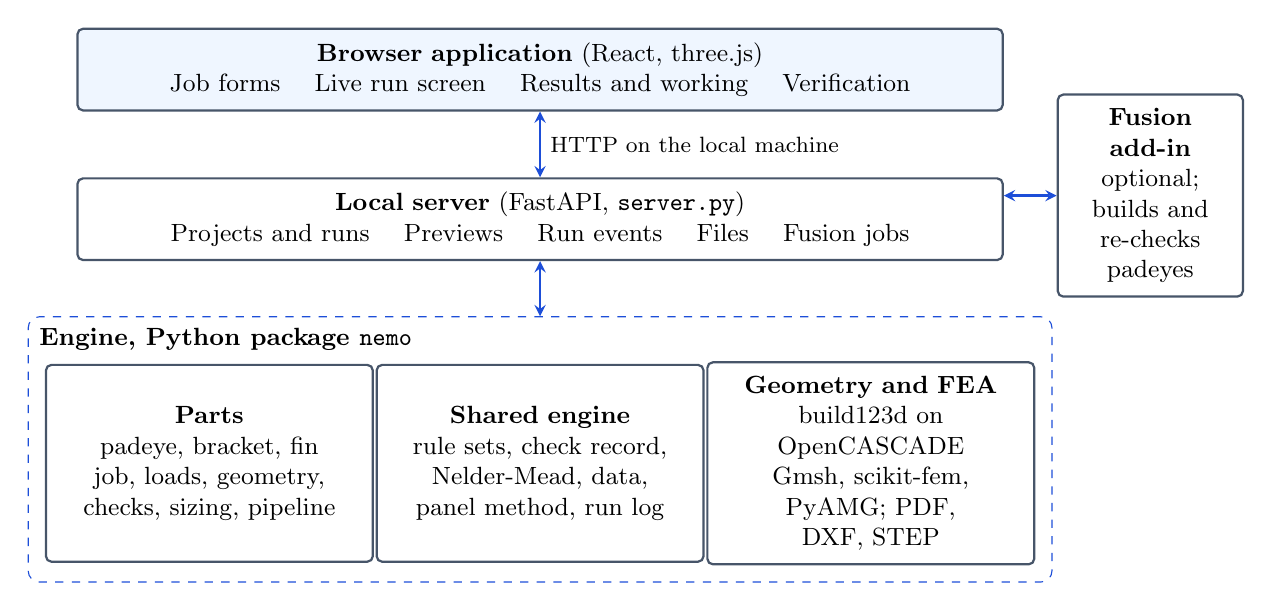
\begin{tikzpicture}[font=\small]
\node[layer, text width=11.4cm, fill=nemolight] (app) at (0,0) {\textbf{Browser application} (React, three.js)\\
Job forms \quad Live run screen \quad Results and working \quad Verification};
\node[layer, text width=11.4cm] (server) at (0,-1.9) {\textbf{Local server} (FastAPI, \code{server.py})\\
Projects and runs \quad Previews \quad Run events \quad Files \quad Fusion jobs};
\node[layer, text width=3.8cm, minimum height=2.5cm] (parts) at (-4.2,-5.0) {\textbf{Parts}\\ padeye, bracket, fin\\ job, loads, geometry,\\ checks, sizing, pipeline};
\node[layer, text width=3.8cm, minimum height=2.5cm] (common) at (0,-5.0) {\textbf{Shared engine}\\ rule sets, check record,\\ Nelder-Mead, data,\\ panel method, run log};
\node[layer, text width=3.8cm, minimum height=2.5cm] (geo) at (4.2,-5.0) {\textbf{Geometry and FEA}\\ build123d on OpenCASCADE\\ Gmsh, scikit-fem,\\ PyAMG; PDF, DXF, STEP};
\coordinate (engtop) at (0,-3.35);
\node[draw=nemoblue, dashed, rounded corners, fit=(parts)(common)(geo)(engtop), inner sep=6pt] (engine) {};
\node[anchor=north west, font=\small\bfseries, inner sep=4pt] at (engine.north west) {Engine, Python package \code{nemo}};
\node[layer, text width=2.0cm] (fusion) at (7.75,-1.6) {\textbf{Fusion add-in}\\ optional;\\ builds and\\ re-checks padeyes};
\draw[arrow, <->] (app) -- node[right, font=\footnotesize] {HTTP on the local machine} (server);
\draw[arrow, <->] (server.south) -- (engine.north -| server.south);
\draw[arrow, <->] (fusion.west) -- (server.east |- fusion.west);
\end{tikzpicture}
\caption{Architecture of \NEMO{}}
\label{fig:architecture}
\end{figure}

\subsection{Engine structure}

Each part is a sub-package of \code{nemo.parts} with the same six modules,
listed in Table~\ref{tab:part-modules}. A registry in
\code{parts/registry.py} lists the parts, so the server and the application
handle all three the same way. Adding a part means writing these modules and
registering them.

\begin{table}[H]
\centering
\caption{Modules that make up one part in the engine}
\label{tab:part-modules}
\small
\begin{tabularx}{\textwidth}{lX}
\toprule
\textbf{Module} & \textbf{What it does}\\
\midrule
\code{job.py} & The job description, its defaults and its validation, and the loads on the part\\
\code{geometry.py} & The design variables, exact areas, volumes and masses, and geometric problems such as a hole too close to an edge\\
\code{checks.py} & Every check on a design, each with its working, returned as a list of check records\\
\code{sizing.py} & The search for the lightest design at a given maximum use, and the three-design shortlist\\
\code{cad.py} & The exact solid in build123d, and the STEP and STL export\\
\code{fea.py} & The supports, loads and assessed region for the finite element model\\
\code{pipeline.py} & One run from start to finish: loads, sizing, CAD, FEA, files and the PDF\\
\bottomrule
\end{tabularx}
\end{table}

The engine has 52 Python files and 9,605 lines of code. The application has
34 TypeScript files and 7,182 lines. The Fusion add-in has 532 lines. The main
libraries and their versions are listed in Table~\ref{tab:software}.

\begin{table}[H]
\centering
\caption{Main software used by \NEMO{}}
\label{tab:software}
\small
\begin{tabularx}{\textwidth}{llX}
\toprule
\textbf{Library} & \textbf{Version} & \textbf{Use in \NEMO{}}\\
\midrule
build123d (OpenCASCADE) & 0.13.0 & Exact solids, volumes, STEP and STL export\\
Gmsh & 4.15.2 & Tetrahedral meshing with local refinement \cite{gmsh2009}\\
scikit-fem & 12.0.2 & Finite element basis functions and assembly \cite{skfem2020}\\
PyAMG & 5.4.1 & Smoothed-aggregation multigrid preconditioner \cite{pyamg2023}\\
NumPy, SciPy & 2.5.5, 1.18.1 & Arrays, sparse matrices, direct sparse solver\\
FastAPI & 0.163.1 & Local web server\\
ReportLab, Matplotlib & 5.1.0, 3.11.2 & PDF calculation package and its plots\\
ezdxf & 1.4.5 & DXF cutting profiles\\
React, three.js & 19, 0.170 & Browser application and 3D views\\
\bottomrule
\end{tabularx}
\end{table}

\subsection{Runs and project files}
\label{sec:run-files}

A project holds the job description. Each time the user presses
\emph{Find designs}, the engine creates a new run folder named after the date
and time, so earlier runs are never overwritten. A padeye run writes the
following files.

\begin{lstlisting}[language={}, numbers=none, caption={Files written by one padeye run}, label={lst:run-folder}]
20270115-090000-000000/
  results.json             loads, every design, every check and its working
  engineering-log.json     time-stamped record of every step of the run
  designs-evaluated.csv    every design the search tried (19,389 rows here)
  designs/
    lightest/  balanced/  robust/
      calculation-report.pdf   the calculation package
      padeye.step  padeye.stl  the exact solid and a mesh for viewing
      padeye-cutting.dxf       cutting profiles for the plates
      stress-surface.json      stress on the surface, for the 3D view
\end{lstlisting}

The bracket writes \code{bracket.step} and \code{bracket-cutting.dxf}, and the
fin writes \code{fin.step}, \code{fin-stock.step} and \code{fin-rib-cutting.dxf}, in the same layout.
\code{fin-stock.step} is the stock alone, as the stress check models it, for an
independent check in Fusion.

\section{Reference data}
\label{sec:reference-data}

All material and catalogue data are stored as data files in
\code{nemo/data}, not in the code. Each entry records its source.
Table~\ref{tab:reference-data} lists them.

\begin{table}[H]
\centering
\caption{Reference data held by the engine}
\label{tab:reference-data}
\small
\begin{tabularx}{\textwidth}{>{\raggedright\arraybackslash}p{0.34\textwidth}X}
\toprule
\textbf{Data} & \textbf{Source and use}\\
\midrule
Structural steels S235, S275, S355 & EN 10025-2:2019, minimum yield by thickness band and minimum tensile strength \cite{en10025}\\
Ship steels Grade~A and AH36 & IACS UR W11 \cite{iacsW11}\\
Stainless steel 316L & EN 10088-2, hot-rolled plate\\
Aluminium 5083-H111 & EN 485-2. In this temper the welded strength equals the parent strength\\
Fin stock 42CrMo4, quenched and tempered & EN 10083-3. Yield falls with diameter, 550~MPa up to 160~mm and 500~MPa from 160~mm to 250~mm. Tensile strength 750~MPa \cite{en10083}\\
Shackles Crosby G-2130 / S-2130, 20 sizes from 0.33~t to 150~t & Crosby catalogue: working load limit, jaw width and pin diameter \cite{crosby2019}\\
Pipe sizes NPS~1/2 to NPS~12 & ASME B36.10M: outside diameter and wall thickness by schedule \cite{asmeB3610}\\
U-bolts M10 to M24, steel class 4.6 and stainless A4-70 & ISO 898-1 for the steel class: tensile strength and threaded tensile area \cite{iso898}\\
Fluids and insulation & Densities of sea water, fresh water, fuel oil, diesel and lubricating oil; mineral wool and calcium silicate insulation\\
Plate stock & Steel plate from 5~mm to 100~mm and aluminium from 5~mm to 50~mm. The yard ticks the thicknesses it holds\\
Minimum fillet weld sizes & AWS D1.1: 3, 5, 6 and 8~mm for parts up to 6, 12 and 19~mm and over 19~mm \cite{awsD11}\\
\bottomrule
\end{tabularx}
\end{table}

\section{The common check model}
\label{sec:check-model}

Every check in \NEMO{}, for every part, is returned as the same record. This is
what lets one application, one report generator and one sizing pattern serve
three different parts. The record holds the following fields.

\begin{itemize}
    \item \textbf{Demand and capacity}, with a unit. The utilisation is
    $U = \text{demand}/\text{capacity}$, and the check passes when
    $U \leq 1$. The spare capacity is $(1-U) \times 100\%$.
    \item \textbf{Source}, the clause or document the capacity comes from,
    such as ``ASME BTH-1, pin-connected plates: bearing strength''.
    \item \textbf{Basis}, either \emph{rule} for a published code or
    \emph{practice} for a project rule. Practice checks print ``NEMO
    practice'' in the source, so a checker can see at once which checks are
    not from a code.
    \item \textbf{Severity}, either \emph{required} or \emph{advice}. A
    failing required check fails the design. A failing advice check appears
    as a warning.
    \item \textbf{Category}: \emph{strength}, \emph{fit} for sizes and
    fit-up, \emph{stiffness} for deflection limits, or \emph{span} for the
    pipe between supports. The sizing targets of
    Section~\ref{sec:sizing} apply to strength checks only.
    \item \textbf{Working}, a list of steps. Each step has the quantity, the
    formula, the formula with the values substituted and the result. The
    application and the PDF print these steps, and a test confirms that the
    result of the last step equals the value the check uses.
\end{itemize}

The \emph{governing} check of a design is the required strength check with the
highest utilisation. Listing~\ref{lst:working} shows, in condensed form, the
working for the base weld check of the case-study padeye. The full steps are in
Figure~\ref{fig:app-check-working}.

\begin{lstlisting}[language={}, numbers=none, caption={Working for one check, condensed}, label={lst:working}]
Base weld strength            ASME BTH-1, welded connections
  Allowable shear on throat   F_w = 0.60 E_xx / (1.20 N_d)
                              = 0.60 x 482 / (1.20 x 3.00) = 80.33 MPa
  Resultant on the throat     f_r = sqrt(f_n^2 + f_s^2) = 78.70 MPa
  Use                         78.70 / 80.33 = 98.0%      passes
\end{lstlisting}

\section{Rule sets}
\label{sec:rule-sets}

A rule set supplies the allowable stresses and safety factors of one design
code. Parts call the rule set and never hold a code's factors themselves. Each
rule set is a small class in \code{nemo/rules} and is chosen by its identifier
in the job, so another code can be added as a module with the same methods.
Table~\ref{tab:rule-sets} summarises the three rule sets.

\begin{table}[H]
\centering
\caption{Rule sets in \NEMO{}}
\label{tab:rule-sets}
\small
\begin{tabularx}{\textwidth}{>{\raggedright\arraybackslash}p{0.2\textwidth}>{\raggedright\arraybackslash}p{0.2\textwidth}X}
\toprule
\textbf{Rule set} & \textbf{Part} & \textbf{Main factors}\\
\midrule
ASME BTH-1 \cite{asmeBTH1} & Lifting padeye & Design factor $N_d = 2.00$ for category~A and $3.00$ for category~B. Pin-connected plates use $1.20N_d$. Welds $0.60E_{xx}/(1.20N_d)$\\
AISC 360-16, ASD \cite{aisc2016} & Pipe support bracket & $\Omega = 1.67$ for tension, flexure and shear yield; $\Omega = 2.00$ for fillet welds on $0.60F_{EXX}$ and for bolts on $0.75F_u$ in tension and $0.45F_u$ in shear\\
IACS UR S10 Rev.8 \cite{iacsS10} & Stabilizer fin & Material factor $k = (235/R_{eH})^{0.75}$ with $R_{eH} \leq \min(0.7\sigma_T, 450)$~MPa. Stock and blade limits are multiples of $1/k$\\
\bottomrule
\end{tabularx}
\end{table}

The fin is not a rudder, but it is an all-movable foil on a stock, which is
the case UR S10 covers. The rudder rules are applied to it as the nearest
published basis, and the report says so on every fin check.

\section{Lifting padeye model}
\label{sec:padeye-model}

\subsection{Geometry}

The padeye is a flat main plate welded to the deck or structure along its base,
with a round head and a hole for a shackle pin
(Figure~\ref{fig:padeye-model}). The outline is the convex hull of the base
line, of length $L$, and the head circle, of radius $R$, centred at hole height
$h$. The hole has diameter $D_h$. Two optional cheek plates, rings of
thickness $t_c$ and outer radius $R_c \leq R$, can be welded on either side of
the head to thicken it at the hole. The thickness at the hole is then
$t = t_\text{main} + 2t_c$.

The area is computed exactly from a polygon through the base corners, the
tangent points and the hole centre, plus the head sector, minus the hole. The
mass is the volume times the density. Weld metal is not counted.

\begin{figure}[H]
\centering
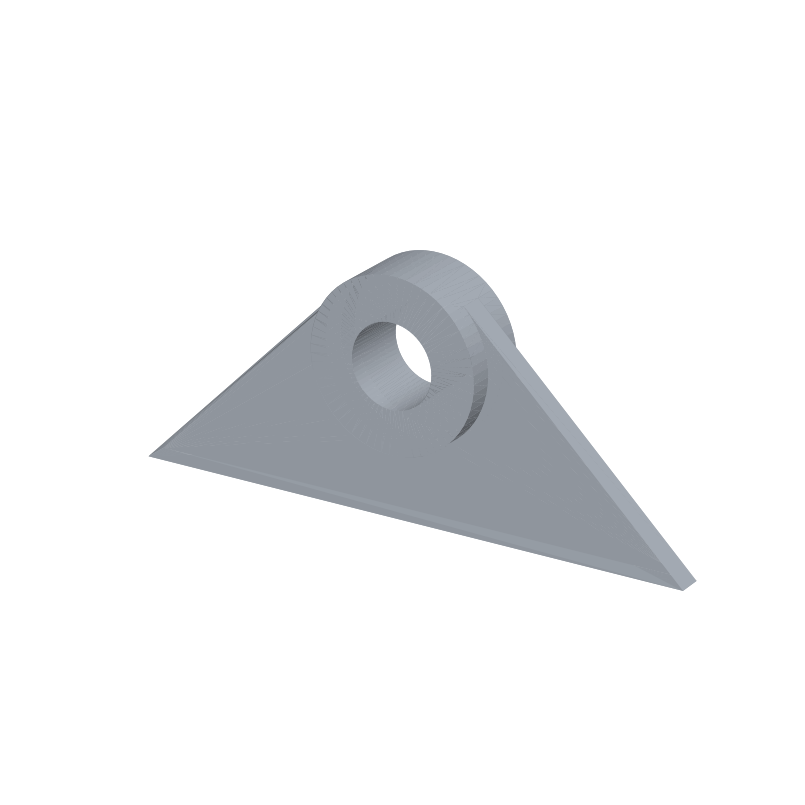
\includegraphics[width=0.62\textwidth]{images/padeye-model.png}
\caption{Lightest case-study padeye, with cheek plates, built by the engine}
\label{fig:padeye-model}
\end{figure}

\subsection{Loads}

The user gives the lifted mass $m$, the number of lifting points, the sling
angle $\theta$ from the horizontal and, if needed, a dynamic factor and the
number of points assumed to carry the load. The force on one padeye follows
from statics.
\begin{align}
V &= \frac{m g \,\text{DAF}}{n_c}, & F &= \frac{V}{\sin\theta}, &
H &= F\cos\theta, & Q &= kF
\label{eq:padeye-loads}
\end{align}
Here $g = 9.80665$~m/s$^2$, DAF is the dynamic factor (default 1.0), $n_c$ is
the number of points carrying the load (default all of them), $V$ and $H$ are
the vertical and in-plane horizontal parts of the sling force $F$, and $Q$ is a
sideways allowance out of the plane of the padeye, with $k = 0.05$ by default.
The sling angle is limited to between 15$^\circ$ and 90$^\circ$. In a simple
lift the plate lies in the plane of its sling.

\subsection{Oblique slings}
\label{sec:oblique-sling}

A padeye fixed to a deck or a structure does not always face its sling. An
oblique sling needs two angles to describe it: the sling angle $\theta$ from
the horizontal, and a second angle $\beta$ between the sling and the plate of
the padeye seen from above. $\beta$ is an advanced setting with a default of
0$^\circ$, the usual case, in which Equation~\eqref{eq:padeye-loads} applies
unchanged. For $\beta > 0$ the sling force is split into
\begin{equation}
H = F\cos\theta\cos\beta, \qquad
Q = F\max(\cos\theta\sin\beta,\; k), \qquad
\gamma = \sin^{-1}(\cos\theta\sin\beta)
\label{eq:oblique}
\end{equation}
where $Q$ is the larger of the real sideways part and the allowance $kF$, and
$\gamma$ is the angle between the sling and the plane of the plate. The base,
shear and weld checks use these $H$ and $Q$. The head checks keep the full
sling force $F$, which is conservative because only $F\cos\gamma$ acts in the
plane of the plate. The finite element model applies the in-plane part
$\sqrt{H^2 + V^2}$ through the hole and $Q$ across it.

The shackle can swing about its pin in the plane of the padeye, but it cannot
swing out of that plane, so $\gamma$ is the side-load angle of the shackle.
Crosby rates screw-pin and bolt-type shackles loaded at an angle to their
in-line axis at a share $r(\gamma)$ of the working load limit
\cite{crosbySideLoad}: 100\% up to 10$^\circ$, 85\% to 20$^\circ$, 75\% to
30$^\circ$, 70\% to 45$^\circ$, 60\% to 55$^\circ$, 55\% to 70$^\circ$ and 50\%
to 90$^\circ$. Shackles larger than 3~in keep the full rating only to
5$^\circ$, 85\% to 10$^\circ$, and need a separate analysis beyond that, which
\NEMO{} treats as not allowed. The shackle is chosen, and the shackle rating is
checked, against $r(\gamma)\,\text{WLL}$.

\subsection{Checks to ASME BTH-1}

The head checks follow the pin-connected plate provisions of ASME BTH-1
\cite{asmeBTH1}. Because the head is a circle concentric with the hole, the
edge distance $R$ and the net width $b_e = R - D_h/2$ are the same in every
in-plane direction. The head checks therefore use the full sling force $F$ for
any sling angle. With cheek plates, the smaller of $R$ and $R_c$ and the lower
yield of the two plates are used. $F_y$ and $F_u$ are the minimum yield and
tensile strengths for the plate thickness and $D_p$ is the shackle pin
diameter.
\begin{align}
C_r &= 1 - 0.275\sqrt{1 - D_p^2/D_h^2}
\label{eq:cr}\\
b_\text{eff} &= \min\!\left(b_e,\; 4t,\; 0.6\,\frac{F_u}{F_y}\sqrt{\frac{D_h}{b_e}}\; b_e\right)
\label{eq:beff}\\
P_t &= \frac{C_r F_u \, 2 t \, b_\text{eff}}{1.20 N_d}
\label{eq:pt}\\
P_b &= \frac{C_r F_u}{1.20 N_d}\left[1.13\left(R - \frac{D_h}{2}\right) + \frac{0.92\, b_e}{1 + b_e/D_h}\right] t
\label{eq:pb}\\
P_v &= \frac{0.70 F_u A_v}{1.20 N_d}, \qquad
A_v = 2\left[a + \frac{D_p}{2}\left(1 - \cos\phi\right) - Z\right] t
\label{eq:pv}\\
P_p &= \frac{C F_y D_p t}{N_d}
\label{eq:pp}
\end{align}
In Equation~\eqref{eq:pv}, $a = R - D_h/2$, $\phi = 55 D_p/D_h$ in degrees,
and $Z = R - \sqrt{R^2 - (D_p \sin\phi/2)^2}$ is the loss of shear plane at the
curved edge. In Equation~\eqref{eq:pp}, $C = 1.25$ for service class~0 and
$0.63$ for classes 1 to 4. Each capacity is compared with $F$.

The base of the main plate, $L$ by $t_\text{main}$, is checked as a
cantilever of length $h$ under $V$, $H$ and $Q$.
\begin{gather}
f_a = \frac{V}{L t}, \quad
f_{bx} = \frac{H h}{t L^2/6}, \quad
f_{by} = \frac{Q h}{L t^2/6}, \quad
f_v = \frac{\sqrt{H^2 + Q^2}}{L t}
\label{eq:base-stress}\\
\frac{f_a}{F_y/N_d} + \frac{f_{bx}}{F_{bx}} + \frac{f_{by}}{1.25F_y/N_d} \leq 1,
\qquad f_v \leq \frac{F_y}{\sqrt{3}\,N_d}
\label{eq:base-combined}
\end{gather}
The strong-axis allowable $F_{bx}$ includes lateral-torsional buckling of the
plate as a rectangular bar. With $\lambda = h L/t^2$, $F_{bx} = 1.25F_y/N_d$ for
$\lambda \leq 0.08E/F_y$, falls linearly as
$[1.52 - 0.274\lambda F_y/E]F_y/N_d$ up to $\lambda = 1.9E/F_y$, and is
$1.9E/(\lambda N_d)$ beyond that.

The fillet welds are checked on the throat against
$F_w = 0.60E_{xx}/(1.20N_d)$, with $E_{xx} = 482$~MPa for E70XX electrodes.
The base weld is two fillet lines of length $L$ with throat $a = 0.707w$ for
leg $w$, their centrelines $t_\text{main} + a$ apart. The normal stress from
$V$, $Hh$ and $Qh$ on this weld group and the shear from $\sqrt{H^2+Q^2}$ are
combined as a vector resultant on the throat. Each cheek plate carries
$F t_c/t$ through one fillet around its circumference $2\pi R_c$.

\subsection{Practice checks}

Some needs of a padeye are not covered by BTH-1. They are checked as
\NEMO{} practice and labelled so in the reports
(Table~\ref{tab:padeye-practice}).

\begin{table}[H]
\centering
\caption{Padeye checks taken from practice and catalogue data}
\label{tab:padeye-practice}
\small
\begin{tabularx}{\textwidth}{lXl}
\toprule
\textbf{Check} & \textbf{Rule} & \textbf{Severity}\\
\midrule
Hole clearance & $D_h \geq D_p + 1$~mm & Required\\
Shackle fit & $t + 2$~mm $\leq$ jaw width & Required\\
Shackle rating & $F/g \leq r(\gamma)\,$WLL, the working load limit reduced for side loading (Section~\ref{sec:oblique-sling}) \cite{crosby2019,crosbySideLoad} & Required\\
Jaw fill & $t \geq 0.6 \times$ jaw width, so the shackle cannot tilt on the pin & Advice\\
Pin fit & $D_p/D_h \geq 0.90$, after the BTH-1 commentary on clearance & Advice\\
Minimum fillet size & AWS D1.1 minimum for the thicker part joined \cite{awsD11} & Advice\\
\bottomrule
\end{tabularx}
\end{table}

\section{Pipe support bracket model}
\label{sec:bracket-model}

\subsection{Geometry}

The bracket is a horizontal seat plate, $L \times b \times t_s$, welded to a
bulkhead and stiffened by two triangular knees of thickness $t_k$
(Figure~\ref{fig:bracket-model}). The knees are flush with the seat edges,
$h_k$ deep at the bulkhead and run out to the seat tip. The pipe sits on the
seat at $e = \text{gap} + \text{insulation} + D/2$ from the bulkhead, held by
a U-bolt of diameter $d$ whose legs pass through holes of $d + 2$~mm at
$x = e \pm (D+d)/2$. The seat length is
$L = e + (D+d)/2 + 1.5d_\text{hole}$, rounded up to 5~mm.

\begin{figure}[H]
\centering
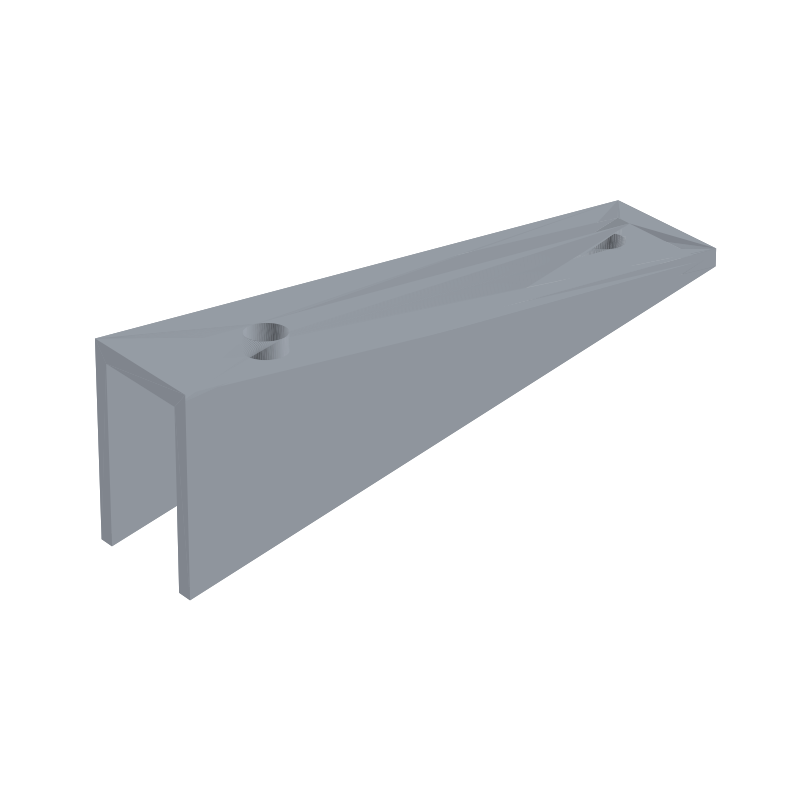
\includegraphics[width=0.6\textwidth]{images/bracket-model.png}
\caption{Lightest case-study pipe support bracket, for an NPS~4 seawater line}
\label{fig:bracket-model}
\end{figure}

\subsection{Loads}

The weight per metre of pipe is $q = g(m_\text{pipe} + m_\text{contents} +
m_\text{insulation})$, with the pipe metal and the bore from ASME B36.10M. One
bracket carries
\begin{equation}
W = k_c\, q\, S
\label{eq:bracket-weight}
\end{equation}
where $S$ is the support spacing and $k_c$ the continuity factor. The default
$k_c = 1.25$ is the middle-support reaction of a two-span continuous beam. Ship
motion adds inertia. The design forces at the pipe are
\begin{equation}
F_z = W(1 + a_v), \quad
F_u = W(a_v - 1) \text{ when } a_v > 1, \quad
F_x = W a_h, \quad
F_y = \mu F_z
\label{eq:bracket-loads}
\end{equation}
for downward, upward, across-pipe and along-pipe directions. The horizontal
acceleration $a_h$ is the athwartships value for a fore-and-aft pipe and the
fore-and-aft value otherwise. Friction $\mu$ (default 0.3) sets the along-pipe
force. The accelerations are inputs. \NEMO{} does not compute them from a
classification society method.

\subsection{Checks to AISC 360-16}

The structural checks use AISC 360-16 in allowable strength design
\cite{aisc2016}. Table~\ref{tab:bracket-checks} lists them. The arm is checked
at 61 stations between the bulkhead and the pipe. At each station the section
is the seat flange plus the two knee webs of depth $h_k(1 - x/L)$. The bending
allowable is taken at first yield, $Z/S = 1$, because the thin knees are not
compact.

\begin{table}[H]
\centering
\caption{Bracket checks}
\label{tab:bracket-checks}
\small
\begin{tabularx}{\textwidth}{>{\raggedright\arraybackslash}p{0.22\textwidth}X}
\toprule
\textbf{Check} & \textbf{Method}\\
\midrule
Arm bending & $U(x) = \dfrac{F_x}{A F_t} + \dfrac{M_y}{S_\text{min} F_b} + \dfrac{M_z}{S_z F_b}$ with $M_y = F_z(e-x) + F_x(D/2 - \bar z)$ and $M_z = F_y(e-x)$; the maximum over the stations (Chapter~H)\\
Arm shear & $V/(2t_k h(x) + b t_s)$ against $0.6F_y/\Omega$ (Chapter~G)\\
Welds to the bulkhead & Line-weld group of two lines across the seat and two per knee. $f_n = N/A_w + M_y c/I_w + M_z(b/2)/I_{wz}$, $f_s = \sqrt{V^2 + F_y^2}/A_w$, resultant on the throat (J2.4)\\
Knee-to-seat welds & Shear flow $VQ/I_y$ at the root over four fillets\\
Seat between the knees & A strip of width $\min(L, b - t_k)$ spanning $l = b - t_k$, $M = \max(F_z l/8,\; T l/4)$, against $1.5F_y/\Omega$ (F11)\\
U-bolt & $T = F_u/2 + F_x(D/2)/s$ per leg and $V = F_x/2$, with $(f_t/F_t)^2 + (f_v/F_v)^2 \leq 1$ (J3.6, J3.7)\\
Deflection & $\delta = \int F_z(e-x)^2/(EI(x))\,dx + \int F_z/(GA_v(x))\,dx$ by Simpson's rule, against a limit set for the job (1~mm by default)\\
Knee free edge (advice) & $l_e \leq 50t_k\sqrt{235/F_y}$, after ship-structure bracket rules\\
Pipe on its brackets (advanced, on by default) & Dunkerley's combined frequency of the span and the bracket at least the margin from every excitation (Section~\ref{sec:bracket-flexibility})\\
\bottomrule
\end{tabularx}
\end{table}

The smallest U-bolt that passes is used, but not less than M10 for pipes under
60~mm outside diameter, M12 under 170~mm, M16 under 280~mm and M20 above. This
is \NEMO{} practice so that a small load does not lead to a U-bolt too slender
to handle.

\subsection{Pipe span checks}
\label{sec:pipe-span}

A bracket can be strong enough while the pipe between two brackets still
fails, most often by resonating with the machinery. \NEMO{} checks the span
as well as the bracket. The first natural frequency of a simply supported
span is
\begin{equation}
f_n = \frac{\pi}{2}\sqrt{\frac{EI}{m S^4}}
\label{eq:span-frequency}
\end{equation}
with $m$ the mass per metre of pipe, contents and insulation. The excitation
frequencies come from the machinery data in the job.
\begin{gather}
f_\text{shaft} = \frac{n_p}{60}, \quad
f_\text{blade} = Z\frac{n_p}{60}, \quad
f_{2\,\text{blade}} = 2Z\frac{n_p}{60}, \quad
f_\text{engine} = \frac{n_e}{60}, \quad
f_\text{firing} = \frac{c\, n_e}{60\,s}
\label{eq:excitations}
\end{gather}
Here $n_p$ and $n_e$ are the propeller and engine speeds in rpm, $Z$ the
number of blades, $c$ the number of cylinders, and $s = 2$ for a four-stroke
engine and 1 for a two-stroke. The span passes when $f_n$ is at least a
margin, 20\% by default, away from every excitation.

Two further checks limit pipe stress and sag. The bending stress
$\sigma = q_d S^2/(10Z)$ uses $q_d = q\sqrt{(1+a_v)^2 + a_h^2}$ and is
compared with $F_{y,\text{pipe}}/1.67$. The sag $5qS^4/(384EI)$ is advised to
stay under 2.5~mm, the figure used in MSS SP-58 style span tables
\cite{mssSP58}. Finally, \NEMO{} reports a recommended maximum spacing, the
smallest of the spans that meet the stress limit, the sag limit and
$f_n \geq (1 + \text{margin})$ times the highest excitation.

Span checks have their own category. The sizing search ignores them, because
the size of the bracket cannot change them, but a failing required span check
still fails the design and is shown first in the results.

\subsection{Bracket flexibility}
\label{sec:bracket-flexibility}

Equation~\eqref{eq:span-frequency} treats the supports as rigid. A real
bracket bends a little under the pipe, and the pipe then vibrates on springs,
at a lower frequency. This is an advanced setting that is on by default,
because it needs no further input. The bracket's stiffness under the pipe and
the pipe mass it carries give it its own frequency, and Dunkerley's method
\cite{blevins1979} combines the two:
\begin{equation}
k = \frac{F_z}{\delta}, \qquad
f_b = \frac{1}{2\pi}\sqrt{\frac{k\,g}{W}}, \qquad
\frac{1}{f^2} = \frac{1}{f_n^2} + \frac{1}{f_b^2}
\label{eq:dunkerley}
\end{equation}
with $\delta$ the deflection of the bracket at the pipe under $F_z$
(Table~\ref{tab:bracket-checks}) and $W$ the static weight on one bracket.
Dunkerley's estimate errs low, which is on the safe side when the span is
meant to stay above the excitations. The combined frequency $f$ must keep the
same margin from every excitation. Unlike the span checks, this one depends on
the bracket, so it is placed in the stiffness category and the sizing search
stiffens the bracket if it fails. When the span already fails on rigid
supports, no bracket can fix it, and the check moves to the span category.

\section{Stabilizer fin model}
\label{sec:fin-model}

\subsection{Geometry}

The fin is a rectangular foil of span $b$ and chord $c$ with a symmetric
NACA four-digit section of thickness ratio $t/c$. Its internal structure is a
plated skin, a front and a rear spar at fixed chord fractions, ribs at a
uniform pitch and a solid stock at chord fraction $x_s/c$ that turns the fin
and carries its load into the bearings in the hull
(Figure~\ref{fig:fin-model}). The ribs follow the inside of the skin.

\begin{figure}[H]
\centering
\begin{subfigure}{0.48\textwidth}
\centering
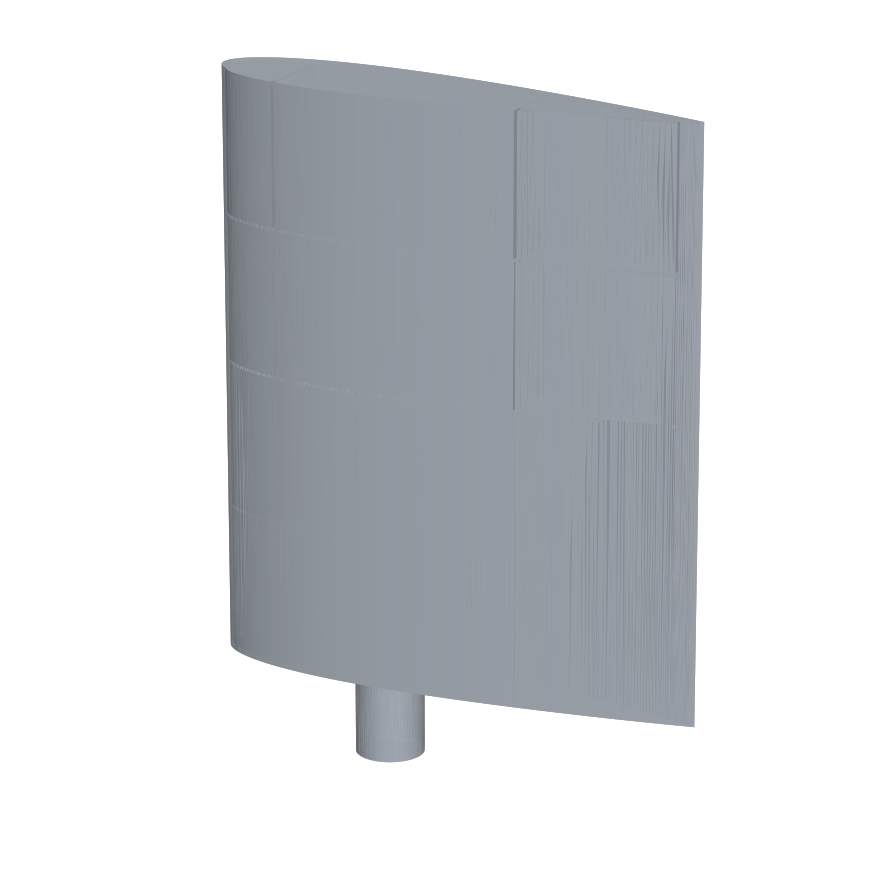
\includegraphics[width=\textwidth]{images/fin-model.png}
\caption{Outside of the fin and the stock}
\end{subfigure}
\hfill
\begin{subfigure}{0.48\textwidth}
\centering
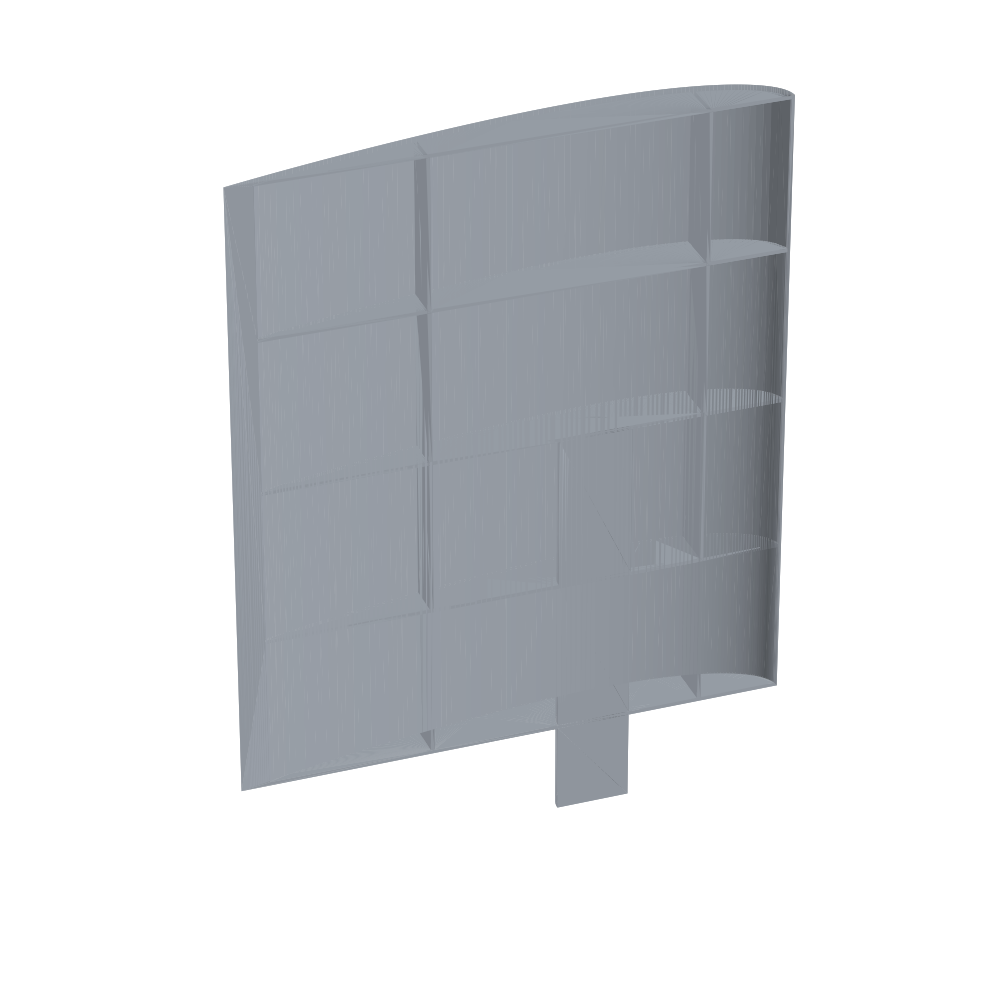
\includegraphics[width=\textwidth]{images/fin-cutaway.png}
\caption{Skin removed to show spars, ribs and stock}
\end{subfigure}
\caption{Lightest case-study stabilizer fin built by the engine}
\label{fig:fin-model}
\end{figure}

\subsection{Loads from two methods}

The fin load is derived twice, by a foil model and by the rule formula, and the
larger is used. This answers requirement R4 and guards against either method
being unconservative for an unusual fin.

The foil model treats the fin as a low-aspect-ratio wing next to the hull. The
hull acts as a mirror plane, so the effective aspect ratio is $A_e = 2b/c$.
Following Whicker and Fehlner \cite{whicker1958}, as used for rudders by
Molland and Turnock \cite{molland2007},
\begin{gather}
\frac{dC_L}{d\alpha} = \frac{0.9 \cdot 2\pi A_e}{\sqrt{A_e^2 + 4} + 1.8},
\qquad
C_L = \frac{dC_L}{d\alpha}\,\alpha + \frac{C_{Dc}}{A_e}\,\alpha^2
\label{eq:whicker}\\
L = \tfrac{1}{2}\rho V^2 A\, C_L
\label{eq:lift}
\end{gather}
where $\alpha$ is the largest fin angle in radians, $C_{Dc} = 0.8$ is the
cross-flow drag coefficient for a square tip, $A = bc$ and
$\rho = 1025$~kg/m$^3$. The second term of $C_L$ is the non-linear lift that a
low-aspect-ratio foil develops at large angles.

The rule formula is the rudder force of IACS UR S10 \cite{iacsS10},
\begin{equation}
C_R = K_1 K_2 K_3 \, 132\, A V^2
\label{eq:ur-force}
\end{equation}
in newtons with $V$ in knots, $K_1 = (\lambda + 2)/3$ with $\lambda = b^2/A$
limited to 2, $K_2 = 1.10$ for a NACA section and $K_3 = 0.8$ for a foil
outside the propeller jet. The design force is $F = \max(L, C_R)$.

The twisting moment on the stock is $Q = F c\,|0.33 - x_s/c|$, at least
$0.1Fc$. The force is taken to act at mid-span, so the bending moment at the
fin root is $M_r = 0.5Fb$ and at the outer bearing
$M_s = F(0.5b + l_g)$, with $l_g$ the gap between the fin root and the
bearing.

\subsection{Astern condition}
\label{sec:astern}

UR S10 requires the rudder force and torque for the astern condition as well
as ahead \cite{iacsS10}. \NEMO{} includes it by default; it needs no input
because the rule sets the least astern speed. With $V_a$ the astern speed, not
less than $0.5V$, $K_2 = 0.80$ for a NACA section astern (UR S10 Table~1), and
the centre of pressure moved aft to 0.66 of the chord (S10.2.1.2),
\begin{equation}
C_{Ra} = K_1 K_2 K_3\,132\,A V_a^2, \qquad
Q_a = C_{Ra}\,c\,|0.66 - x_s/c|, \qquad
M_{sa} = C_{Ra}(0.5b + l_g)
\label{eq:astern}
\end{equation}
The astern force is much smaller than the ahead force, but its lever about
the stock is larger, so for a stock placed well forward the astern twist can
exceed the ahead twist. The stock checks are made for both conditions and
report the worse one. The user can enter a higher astern speed, or switch the
condition off for a fin that is always centred and locked astern.

\subsection{Stock bearings}
\label{sec:bearings}

The stock passes through two bearings in the hull: an outer bearing at
$l_g$ from the fin root and an inner bearing $l$ further in. Sizing them is an
advanced setting, off by default, because $l$ and the bearing material are
often not known at the first design stage. With $a = 0.5b + l_g$ the lever from
the outer bearing to the fin force, the bearing reactions are
\begin{equation}
P_1 = F\,\frac{a + l}{l}, \qquad P_2 = F\,\frac{a}{l}
\label{eq:bearings}
\end{equation}
UR S10.8.2 requires a projected bearing area of at least $P/q_a$, with the
allowable surface pressure $q_a$ from its Table~3: 2.5~N/mm$^2$ for lignum
vitae, 4.5 for white metal, 5.5 for synthetic material harder than 60 Shore~D,
and 7.0 for steel or bronze. The bearing diameter $d_b$ is the stock plus two
liners of the least thickness in S10.8.1, 8~mm (22~mm for lignum). The least
bearing length is then $L = P/(q_a d_b)$, and S10.8.3 limits it to
$1.2\,d_b$. If the length would exceed that, the stock is made larger, which
widens the bearing. The working also gives the least bearing clearance on the
diameter from S10.8.4.

\subsection{Panel method for pressure and cavitation}

The lift formula gives the force but not the pressure on the foil, and
cavitation depends on the lowest pressure. \NEMO{} solves the section with the
Hess-Smith panel method \cite{hess1967}. The section outline is divided into
160 panels with cosine spacing, each carrying a constant source strength, with
one vortex strength shared by all panels. The Kutta condition at the trailing
edge closes the system. The section angle that gives the fin's lift
coefficient is found by solving for the two-dimensional lift slope, and the
pressure distribution at that angle gives $C_{p,\text{min}}$. Cavitation is
flagged when
\begin{equation}
-C_{p,\text{min}} > \sigma = \frac{p_a + \rho g h - p_v}{\tfrac{1}{2}\rho V^2}
\label{eq:cavitation}
\end{equation}
with $p_a = 101.3$~kPa the atmospheric pressure, $h$ the depth of the fin
below the surface and $p_v = 1.7$~kPa the vapour pressure of sea water at
about 15$^\circ$C. This is an advice check.
An inviscid panel method cannot model separated or cavitating flow, so the
check warns of cavitation onset and does not predict its extent.

\subsection{Structural checks}

The fin body between the spars is treated as a box girder. Its second moment
of area is $I = 2\int t y^2\, ds + t_w(h_f^3 + h_r^3)/12$, where the integral
runs along the skin between the spars and $h_f$ and $h_r$ are the spar depths.
The checks are listed in Table~\ref{tab:fin-checks}. The stress limits of UR
S10 are given as multiples of $1/k$.

\begin{table}[H]
\centering
\caption{Stabilizer fin checks}
\label{tab:fin-checks}
\small
\begin{tabularx}{\textwidth}{>{\raggedright\arraybackslash}p{0.22\textwidth}X}
\toprule
\textbf{Check} & \textbf{Method}\\
\midrule
Stock torsion & $\tau_t = 5.1Q/D^3 \times 10^3 \leq 68/k$ (S10.4.1), ahead and astern\\
Stock combined & $\sigma_b = 10.2M_s/D^3 \times 10^3$, $\sigma_e = \sqrt{\sigma_b^2 + 3\tau_t^2} \leq 118/k$ (S10.4.2), ahead and astern\\
Stock bearings (advanced) & $L = P/(q_a d_b) \leq 1.2\,d_b$ for the outer and inner bearing (S10.8.2, 8.3)\\
Stock fit & The stock diameter is less than the foil thickness at the stock position (practice)\\
Fin body bending & $\sigma_b = M_r y/I \leq 110/k$ (S10.5.1)\\
Spar web shear & $F/(t_w\sum h) + q_t/t_w \leq 50/k$, with Bredt shear flow $q_t = Q/(2A_\text{box})$ (S10.5.1)\\
Skin combined & $\sigma_e \leq 120/k$ (S10.5.1)\\
Skin plating & $t \geq 5.5\, s\beta\sqrt{(T + C_R 10^{-4}/A)k} + 2.5$ (S10.5.2)\\
Web thickness & $t_w \geq \max(0.7t, 8~\text{mm})$ (S10.5.2)\\
Skin buckling & $\sigma_E = k_b\pi^2E/[12(1-\nu^2)](t/b_p)^2$ with $k_b = \min_m (m b_p/a_p + a_p/(m b_p))^2$, Johnson-Ostenfeld correction above $F_y/2$, factor 1.5 (practice, after Timoshenko and Gere \cite{timoshenko1961})\\
Tip deflection & Point load at mid-span on a cantilever with the box $I$, against a job limit\\
Cavitation (advice) & $-C_{p,\text{min}} \leq \sigma$\\
\bottomrule
\end{tabularx}
\end{table}

In the plating formula, $s$ is the shorter side of a skin panel bounded by
the ribs and spars, $\beta$ a correction for the panel aspect ratio and $T$
the draught in metres. In the buckling check, $a_p$ is the rib pitch and $b_p$
the spar spacing. The skin and web thicknesses must
come from the plate stock. The stock diameter is not taken from stock lists,
because stocks are forged and turned to size.

\section{Sizing method}
\label{sec:sizing}

\subsection{Problem form}

Each part is sized as a mixed problem. Some variables are discrete because
the yard can only use certain sizes. These are the plate thicknesses from the
ticked stock list, the shackle and U-bolt sizes and the standard weld legs. The rest are
continuous, such as the head radius or the knee depth, but must be rounded to
sizes a workshop can mark out. The objective is the steel mass. The
constraints are the required checks, with strength checks held to a target
maximum use.

\NEMO{} handles the two kinds of variable separately. It enumerates the
discrete choices, and for each combination it sizes the continuous variables
with a bounded Nelder-Mead search \cite{nelder1965,lagarias1998}. Nelder-Mead
needs only the objective value, so it works with checks that have corners,
such as the maximum over 61 stations of the arm, and with designs that switch
governing checks. Figure~\ref{fig:sizing-flow} shows the procedure.

\begin{figure}[H]
\centering
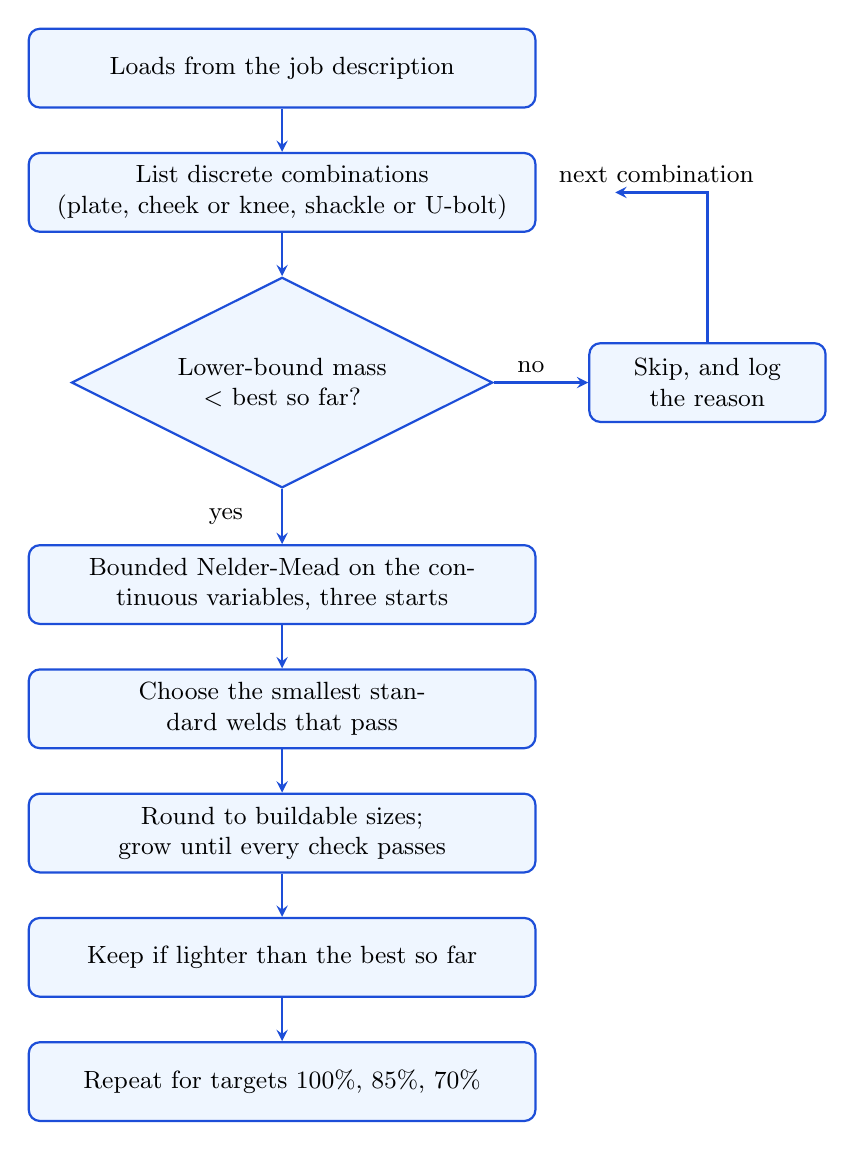
\begin{tikzpicture}[node distance=0.55cm, font=\small, every node/.style={text width=6.2cm}]
\node[startstop] (loads) {Loads from the job description};
\node[process, below=of loads] (discrete) {List discrete combinations\\(plate, cheek or knee, shackle or U-bolt)};
\node[decision, below=of discrete, text width=3.4cm] (bound) {Lower-bound mass $<$ best so far?};
\node[process, below=0.7cm of bound] (nm) {Bounded Nelder-Mead on the continuous variables, three starts};
\node[process, below=of nm] (welds) {Choose the smallest standard welds that pass};
\node[process, below=of welds] (round) {Round to buildable sizes; grow until every check passes};
\node[process, below=of round] (keep) {Keep if lighter than the best so far};
\node[startstop, below=of keep] (out) {Repeat for targets 100\%, 85\%, 70\%};
\node[process, right=1.2cm of bound, text width=2.6cm] (skip) {Skip, and log the reason};
\draw[arrow] (loads) -- (discrete);
\draw[arrow] (discrete) -- (bound);
\draw[arrow] (bound) -- node[left, text width=0.8cm] {yes} (nm);
\draw[arrow] (bound) -- node[above, text width=0.6cm] {no} (skip);
\draw[arrow] (nm) -- (welds);
\draw[arrow] (welds) -- (round);
\draw[arrow] (round) -- (keep);
\draw[arrow] (keep) -- (out);
\draw[arrow] (skip.north) |- ([xshift=1cm]discrete.east) node[pos=0.75, above, text width=2.6cm] {next combination};
\end{tikzpicture}
\caption{Sizing procedure used for every part}
\label{fig:sizing-flow}
\end{figure}

\subsection{Bounded Nelder-Mead search}

The continuous variables are scaled to $[0, 1]$ between bounds that depend on
the combination. For the padeye, the head radius runs from
$D_h/2 + \max(0.25D_h, 5)$ to $D_h/2 + 3D_h + 30$~mm, the base length from
$2R$ to $8R$ and, with cheek plates, the cheek radius from $D_h/2 + 10$~mm to
$R$. For the bracket, the knee depth runs from $0.3L$ to $1.5L$ and the seat
width from $2t_k + 2d + 10$~mm to the larger of $3D$ and that minimum plus
150~mm. Every trial point is clipped to the unit box.

The initial simplex has a step of 0.15 in each scaled variable. The search
uses the standard reflection, expansion, contraction and shrink steps with
coefficients 1, 2, 0.5 and 0.5, and stops when the values and the simplex have
both collapsed, or after 200 iterations for the padeye and 160 for the
bracket. Values are cached, so a repeated point costs nothing. Each
combination is searched from three starting points and the best result kept,
because the feasible region can have several pockets.

Constraints enter through a penalty,
\begin{equation}
\Phi(\mathbf{x}) = m(\mathbf{x})\left[1 + 1000 \sum_i \max(U_i - U_{\text{lim},i},\, 0)^2\right]
\label{eq:penalty}
\end{equation}
summed over the required checks, where $U_{\text{lim},i}$ is the target for
strength checks and 1.0 for the others. A design with a geometric problem,
such as a hole that breaks out of the head, scores $10^9$ and is never kept.
The penalty only guides the search. The design that is finally kept is
re-checked after rounding, and only a design that passes every required check
at the target is accepted.

\subsection{Welds, rounding and pruning}

The search evaluates each trial with a reference weld size. The weld leg is
then set to the smallest standard size, between 3~mm and 20~mm, that passes,
is at least the AWS D1.1 minimum for the thicker part and does not exceed a
practical maximum. The base weld of a padeye is limited to $0.75t_\text{main}$
and a cheek weld to $t_c$.

After the search, the continuous variables are rounded up. For the padeye,
$R$, $R_c$ and $h$ are rounded to 1~mm and $L$ to 5~mm. For the bracket, the
knee depth and seat width are rounded to 5~mm. If the rounded design fails at
the target, it is grown in small steps, 2\% in radius and 3\% in length for
the padeye, and checked again, up to 40 times.

Before a combination is searched, \NEMO{} computes the smallest mass it could
possibly have, for example the padeye with the smallest allowed head and the
shortest base. If that lower bound is already heavier than the best design
found so far, the combination is skipped and the reason is written to the
log. In the bracket case study this pruning skipped 60 of 63 combinations.

\subsection{Fin sizing}

The fin search is exhaustive because its variables are few and its checks
are cheap. For each target, the stock diameter is the smallest 5~mm step that
passes both stock checks, ahead and astern, and, when the bearing check is on,
leaves room for bearings no longer than $1.2\,d_b$. Every pair of skin and web thickness from the stock
list, with webs of at least 8~mm, is then combined with every rib spacing from
150~mm to 1000~mm in 25~mm steps, and the lightest passing fin is kept.

\subsection{Three designs}

The sizing is repeated with strength targets of 100\%, 85\% and 70\% maximum
use. The results are offered as \emph{Lightest}, \emph{Balanced (at least 15\%
spare)} and \emph{Extra margin (at least 30\% spare)}. The targets apply on top
of the code's own safety factors. They let the engineer trade mass against
reserve for uncertain loads, corrosion allowance or future changes without
rerunning the search.

\section{Geometry and output files}
\label{sec:cad}

Each kept design is built as an exact solid with build123d, a Python CAD
library on the OpenCASCADE kernel. The padeye is extruded from its outline,
with the hole cut and the cheek rings added. The bracket is the seat and two
knees, with the U-bolt holes. The fin skin is the NACA outline extruded along
the span, less its inside offset by the skin thickness. The spars, the ribs
and the stock are added to it as solids.

The volume of the solid is compared with the formula the mass came from. The
padeye and the bracket match exactly, which checks the geometry code against
the mass code. The fin's mass uses a thin-wall formula. It takes the skin as
its outer perimeter times its thickness and each rib as the full foil area,
and it counts the stock, spars and ribs again where they overlap. The solid
removes these overlaps, so it is about 3.5\% smaller and the mass formula errs
on the heavy side. The difference is shown on the run screen and in the
report.

From the solid, \NEMO{} writes a STEP file for CAD and fabrication systems and
an STL file for the 3D view. A DXF file gives the cutting profiles of the
plates, the padeye plate and cheeks, the bracket seat and knees, or the fin
ribs, with the hole positions.

\section{Built-in finite element analysis}
\label{sec:fea}

\subsection{Mesh and elements}

The same solid that is written to STEP is meshed with Gmsh \cite{gmsh2009}.
The mesh is refined where the stress is expected to change fastest, around
the hole of the padeye and near the bulkhead for the bracket. The fin stock
is a plain shaft and is meshed uniformly. Each design is meshed three times,
with the element size multiplied by 1.0, 0.7 and 0.5.

The displacement field uses quadratic (P2) tetrahedra in scikit-fem
\cite{skfem2020}, with linear elastic isotropic material. Quadratic elements
are used because linear tetrahedra are too stiff in bending, which matters for
the thin plates of all three parts. The stiffness matrix is assembled by a
vectorised routine that builds all element matrices from the shape-function
gradients with a few array operations. A test confirms that it gives the same
matrix as the scikit-fem reference assembly to within $10^{-12}$.

\subsection{Loads and supports}

Loads are applied as surface tractions defined by a \emph{shape} and a target
resultant. The solver integrates the shape over the loaded faces, then scales
it so that its resultant equals the target. The applied total then matches
the design force used by the checks, whatever the mesh. In the padeye case
study it differed by less than 1~N in each direction. This removes the load
transcription error seen during early exploratory testing (requirement R2).

\begin{itemize}
    \item \textbf{Padeye.} The base face is fixed. The in-plane pin load is a
    cosine pressure $p \propto \max(\cos\alpha, 0)$ on the loaded half of the
    hole surface, with $\alpha$ measured from the sling direction, scaled to
    the in-plane sling force. The sideways force $Q$ is applied as a uniform
    axial traction around the full hole bore so that it introduces no spurious
    twisting moment about the pinhole and matches Autodesk Fusion's Bearing
    Load axial distribution.
    \item \textbf{Bracket.} The faces against the bulkhead are fixed. $F_z$,
    $F_x$ and $F_y$ are uniform tractions on a strip of the seat top under the
    pipe, of width the larger of $D/4$, $2.5t_s$ and 1.5 element sizes.
    \item \textbf{Fin stock.} The model is the stock alone, a solid shaft from
    the outer bearing to $0.6b$, fixed at the bearing face. The fin force and
    the twist are tractions on the stock surface between $0.4b$ and $0.6b$.
    The twist is a load whose force resultant is zero, so it is scaled to its
    target moment instead. On a coarse mesh the scaled twist adds a small net
    force. The force load takes up the part of it along the fin force, and the
    rest is reported with the applied total. In the case study it was 1.2\%
    of the fin force on the coarsest mesh and 0.03\% on the finest.
\end{itemize}

\subsection{Solver}

Below 6,000 unknowns the system is solved directly with SciPy's sparse
solver. Larger systems use conjugate gradients preconditioned by
smoothed-aggregation algebraic multigrid from PyAMG
\cite{pyamg2023,vanek1996}, with the six rigid-body modes as the near-null
space, to a relative residual of $10^{-10}$. If the residual has not fallen
below $10^{-8}$ after 600 iterations, the solver falls back to the direct
method. The residual history is written to the engineering log.

\subsection{Results and acceptance}

The six symmetric Cauchy stress tensor components are evaluated at element
corners, averaged at each vertex, and then combined into the nodal von Mises
stress. Averaging the tensor components before computing von Mises matches
standard finite element post-processors and avoids upward scalar-averaging bias
at geometric transitions. After each solve, \NEMO{} records the following.

\begin{itemize}
    \item \textbf{Force and moment balance}, $|\mathbf{F}_\text{applied} +
    \mathbf{R}|/|\mathbf{F}_\text{applied}|$ and the variational moment
    balance $|\mathbf{M}_\text{applied} +
    \mathbf{M}_R|/|\mathbf{M}_\text{applied}|$, where $\mathbf{R}$ and
    $\mathbf{M}_R$ are the support reaction force and moment. Both must close
    to near zero.
    \item \textbf{Mesh convergence}, the change in the assessed peak stress
    between the two finest meshes. The target is 5\% or less.
    \item \textbf{Assessed peak}, the highest von Mises stress in a stated
    region. Sharp 90$^\circ$ transitions where a fixed face meets a free face,
    and where an unmodeled fillet weld leaves a 90$^\circ$ re-entrant step at
    the outer edge of a padeye cheek plate, carry linear-elastic stress
    singularities that diverge as the mesh is refined. Each part therefore
    reads its peak clear of those singular edges. The assessed region is within
    $R + 1$~mm of the hole axis for the padeye (excluding the 90$^\circ$
    cheek-plate step at $r = R_c$, $|y| = t/2$), at $x \geq 1.5$ times the
    thicker plate for the bracket, and from half a diameter outboard of the
    bearing to the loaded length for the stock.
\end{itemize}

A design passes the finite element check when the assessed peak is below
the yield stress and the meshes have converged. For the bracket and the fin
the peak is also compared with the hand stress at the same place, the seat
bending stress and the stock beam stress respectively. The finite element
analysis confirms the hand checks. It does not replace them, because the code
capacities include effects such as fracture and lateral buckling that a
linear model does not capture.

\begin{figure}[H]
\centering
\begin{subfigure}{0.32\textwidth}
\centering
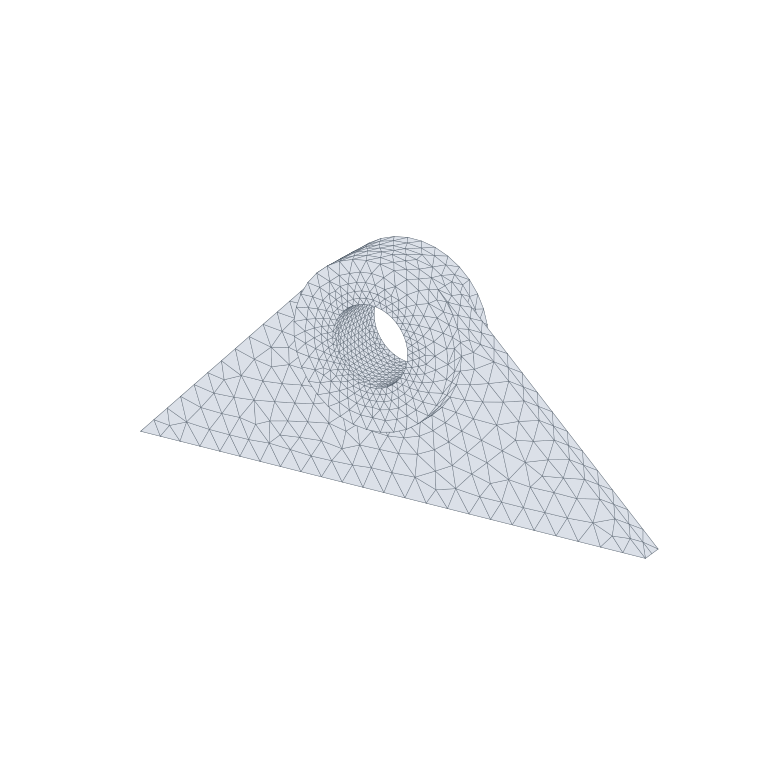
\includegraphics[width=\textwidth]{images/padeye-mesh.png}
\caption{Padeye}
\end{subfigure}
\hfill
\begin{subfigure}{0.32\textwidth}
\centering
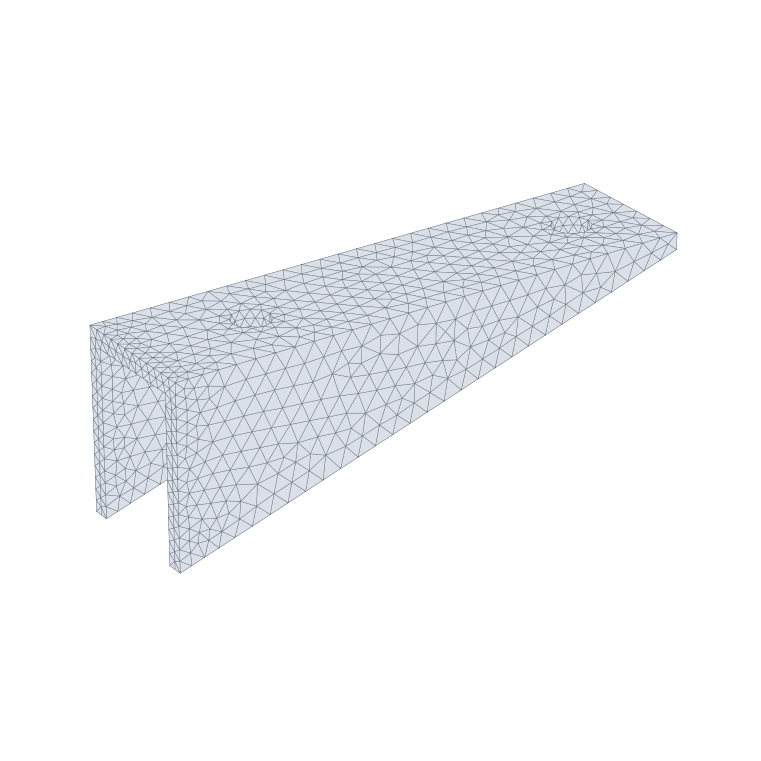
\includegraphics[width=\textwidth]{images/bracket-mesh.png}
\caption{Bracket}
\end{subfigure}
\hfill
\begin{subfigure}{0.32\textwidth}
\centering
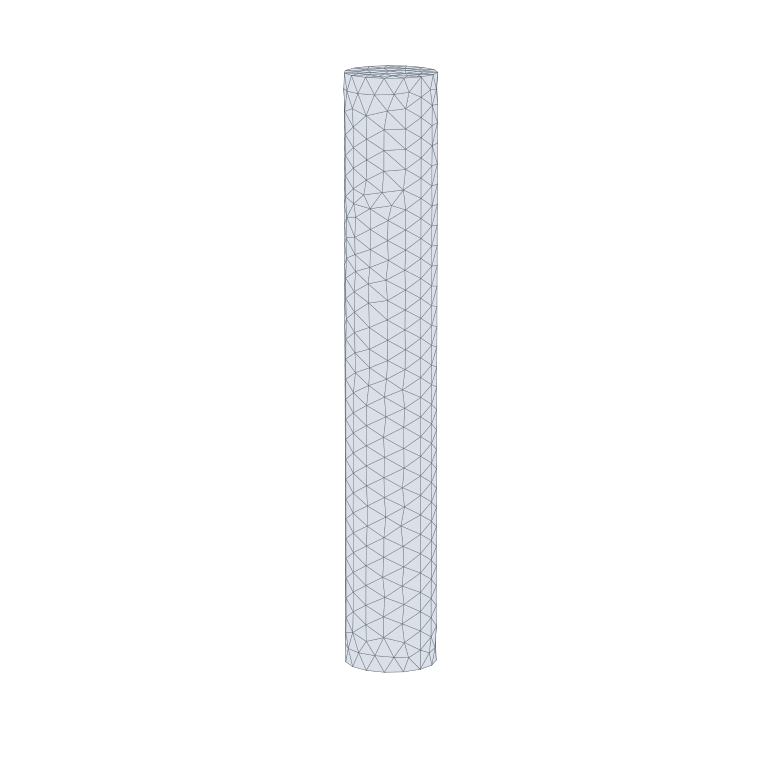
\includegraphics[width=\textwidth]{images/fin-stock-mesh.png}
\caption{Fin stock}
\end{subfigure}
\caption{Finest of the three meshes for each case-study design}
\label{fig:meshes}
\end{figure}

\section{Verification method}
\label{sec:verification-method}

Verification here means checking that the code solves its equations
correctly, as distinct from validation against physical behaviour
\cite{asmeVV10}. Two kinds of evidence were produced.

\textbf{Benchmark suite.} The module \code{nemo.verification} runs the
reference problems in Table~\ref{tab:benchmarks} and reports, for each
quantity, the reference value, the \NEMO{} value, the difference and the
tolerance. The same suite runs from the Verification page of the application,
on the user's own computer, so a checker can confirm the installation they are
using.

\begin{table}[H]
\centering
\caption{Verification benchmarks}
\label{tab:benchmarks}
\small
\begin{tabularx}{\textwidth}{>{\raggedright\arraybackslash}p{0.26\textwidth}>{\raggedright\arraybackslash}X>{\raggedright\arraybackslash}p{0.2\textwidth}}
\toprule
\textbf{Benchmark} & \textbf{What it checks} & \textbf{Reference}\\
\midrule
Padeye hand calculation & Every BTH-1 quantity for a 4~t lift on two points at 60$^\circ$, S355, 20~mm plate, tolerance 0.1\% & Hand calculation in the engineering manual\\
CAD volume & Solid volume of a plain padeye, a padeye with cheeks and a bracket against the exact formula, tolerance 0.01\% & Exact geometry\\
Cantilever & 200 by 20 by 20~mm beam under 1~kN: tip deflection (3\%) and mid-span bending stress (4\%) & Timoshenko beam theory \cite{timoshenko1972}\\
Plate with a hole & 200~mm plate, 20~mm hole, in tension: stress concentration factor, tolerance 5\% & Heywood, in Peterson \cite{peterson2008}\\
Panel method & $C_{p,\text{min}} = -3$ on a circle (0.5\%); lift slope $2\pi(1 + 0.77t/c)$ for NACA~0012 and NACA~0020 (3\%) & Potential flow; Abbott and von Doenhoff \cite{abbott1959}\\
Fin stock & Equivalent stress near the bearing under bending and twist, tolerance 4\% & Beam and torsion theory, as in UR S10.4\\
Support reactions & In every finite element benchmark, the reaction equals the applied load & Statics\\
\bottomrule
\end{tabularx}
\end{table}

\textbf{Automated tests.} The engine has 181 tests in 15 files, run with
pytest after every change. They cover the hand calculation, the behaviour of
the checks when one input changes, CAD volumes for 50 random designs, STEP
export and re-import, the finite element benchmarks, sizing, the working
steps, the run pipeline, the server routes for all three parts, the Fusion
job queue, and each advanced setting against a hand calculation.

\section{Traceability}
\label{sec:traceability}

The tool is meant to be checked by someone who did not write it. Each run
therefore keeps the following records, which answer requirement R9.

\begin{itemize}
    \item \textbf{Working for every check}, as described in
    Section~\ref{sec:check-model}, shown in the application and printed in the
    PDF.
    \item \textbf{Engineering log}, \code{engineering-log.json}, an ordered and
    time-stamped list of events. It records the forces, the shackle or U-bolt choice,
    each search combination and its outcome, thinned samples of designs tried,
    CAD volumes, mesh statistics, solver residual history, force balance and
    mesh convergence. The live run screen of the application is drawn from
    these events as they happen.
    \item \textbf{Every design tried}, \code{designs-evaluated.csv}, with the
    target, discrete choices, dimensions, weld sizes, mass, highest use and
    whether the design met its target.
    \item \textbf{Checksums.} The audit section of the PDF lists the SHA-256
    hash of each run file, so a later change to a file can be detected.
\end{itemize}

The PDF calculation package for each design has a summary page, a
dimensioned drawing, the loads with their working, every check with its
working and source, the finite element results with the mesh study, the
pipe-span or foil results where they apply, the assumptions and limits, and
the audit trail. Examples are shown in Section~\ref{sec:results-package}.

\section{Application and user workflow}
\label{sec:application}

The application is written for an engineer or technician who does not
program. It is installed by double-clicking \code{Install NEMO.bat}. The
installer uses uv to download a private copy of Python~3.12, creates the
engine's environment, installs the libraries, prepares the application and
adds a desktop shortcut. It does not change any other Python on the computer.
\code{Start NEMO.bat} starts the local server and opens the application in the
browser.

The workflow has six screens, in order.

\begin{enumerate}
    \item \textbf{Home} lists the saved projects and starts a new one
    (Figure~\ref{fig:app-home}).
    \item \textbf{New design} asks which part to design.
    \item \textbf{Describe the job} is a form in plain words, such as ``How
    heavy is the load?'' or ``Which plate thicknesses does your workshop
    have?'', with help text and a live 3D preview that updates as values
    change (Figures~\ref{fig:app-describe} and~\ref{fig:app-bracket-motion}). Inputs are validated in the form
    and again by the engine.
    \item \textbf{Assumptions} sets the design basis, with defaults: the rule
    set and, for a padeye, the design category, service class, dynamic factor
    and jaw fill. The bracket and fin have their own versions of this screen.
    Considerations that a simple job does not need sit in a collapsed
    \emph{Advanced settings} section on these screens, with defaults that
    leave a simple job unchanged: the oblique sling angle and load sharing for
    a padeye, the bracket's flexibility in the vibration check, and the fin's
    astern condition and stock bearings.
    \item \textbf{Finding designs} is the live run screen
    (Figure~\ref{fig:app-running}). Each engineering step shows its numbers as
    they are produced, and selecting a step shows its working.
    \item \textbf{Results} shows the three designs, their dimensions, the 3D
    model and stress plot, every check with its working, the engineering
    record and the PDF, and offers the files for download.
\end{enumerate}

A Verification page, reached from the top bar, runs the benchmark suite.
The interface uses one neutral colour scheme with a dark mode and the Inter
typeface. Eleven documents, written in plain language, come with the tool,
including a getting-started guide, a user guide of 1,662 words, an
engineering manual of 3,089 words for checkers, a page each on brackets and
fins, a limits-and-safety page, a glossary and a troubleshooting guide.

\begin{figure}[H]
\centering
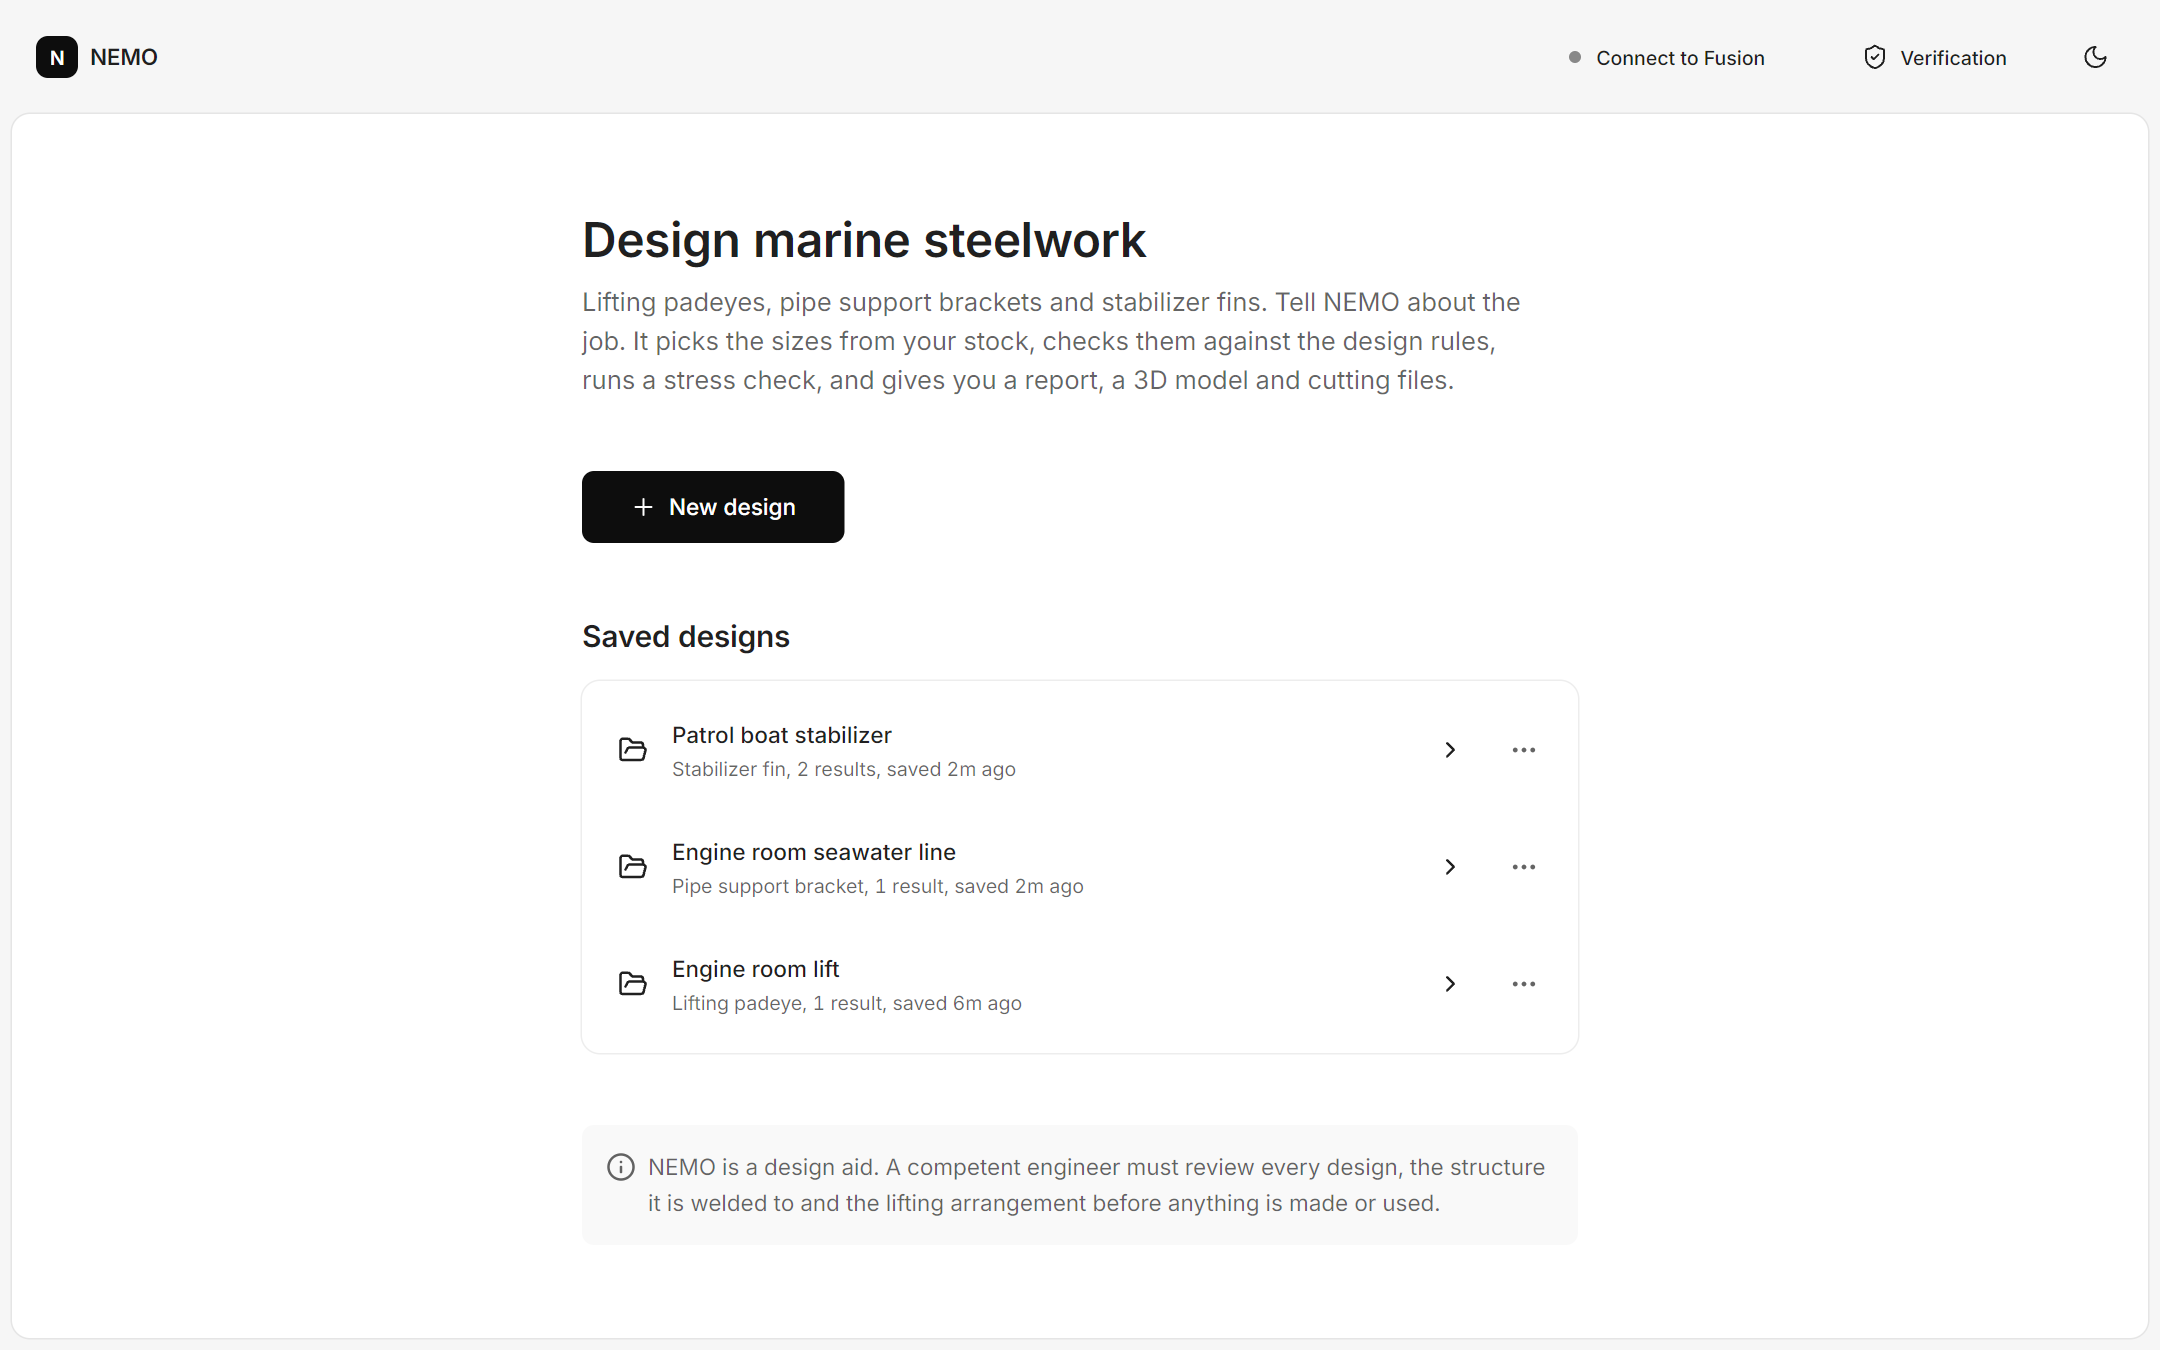
\includegraphics[width=\textwidth]{images/app-home.png}
\caption{Home screen with the three case-study projects}
\label{fig:app-home}
\end{figure}

\begin{figure}[H]
\centering
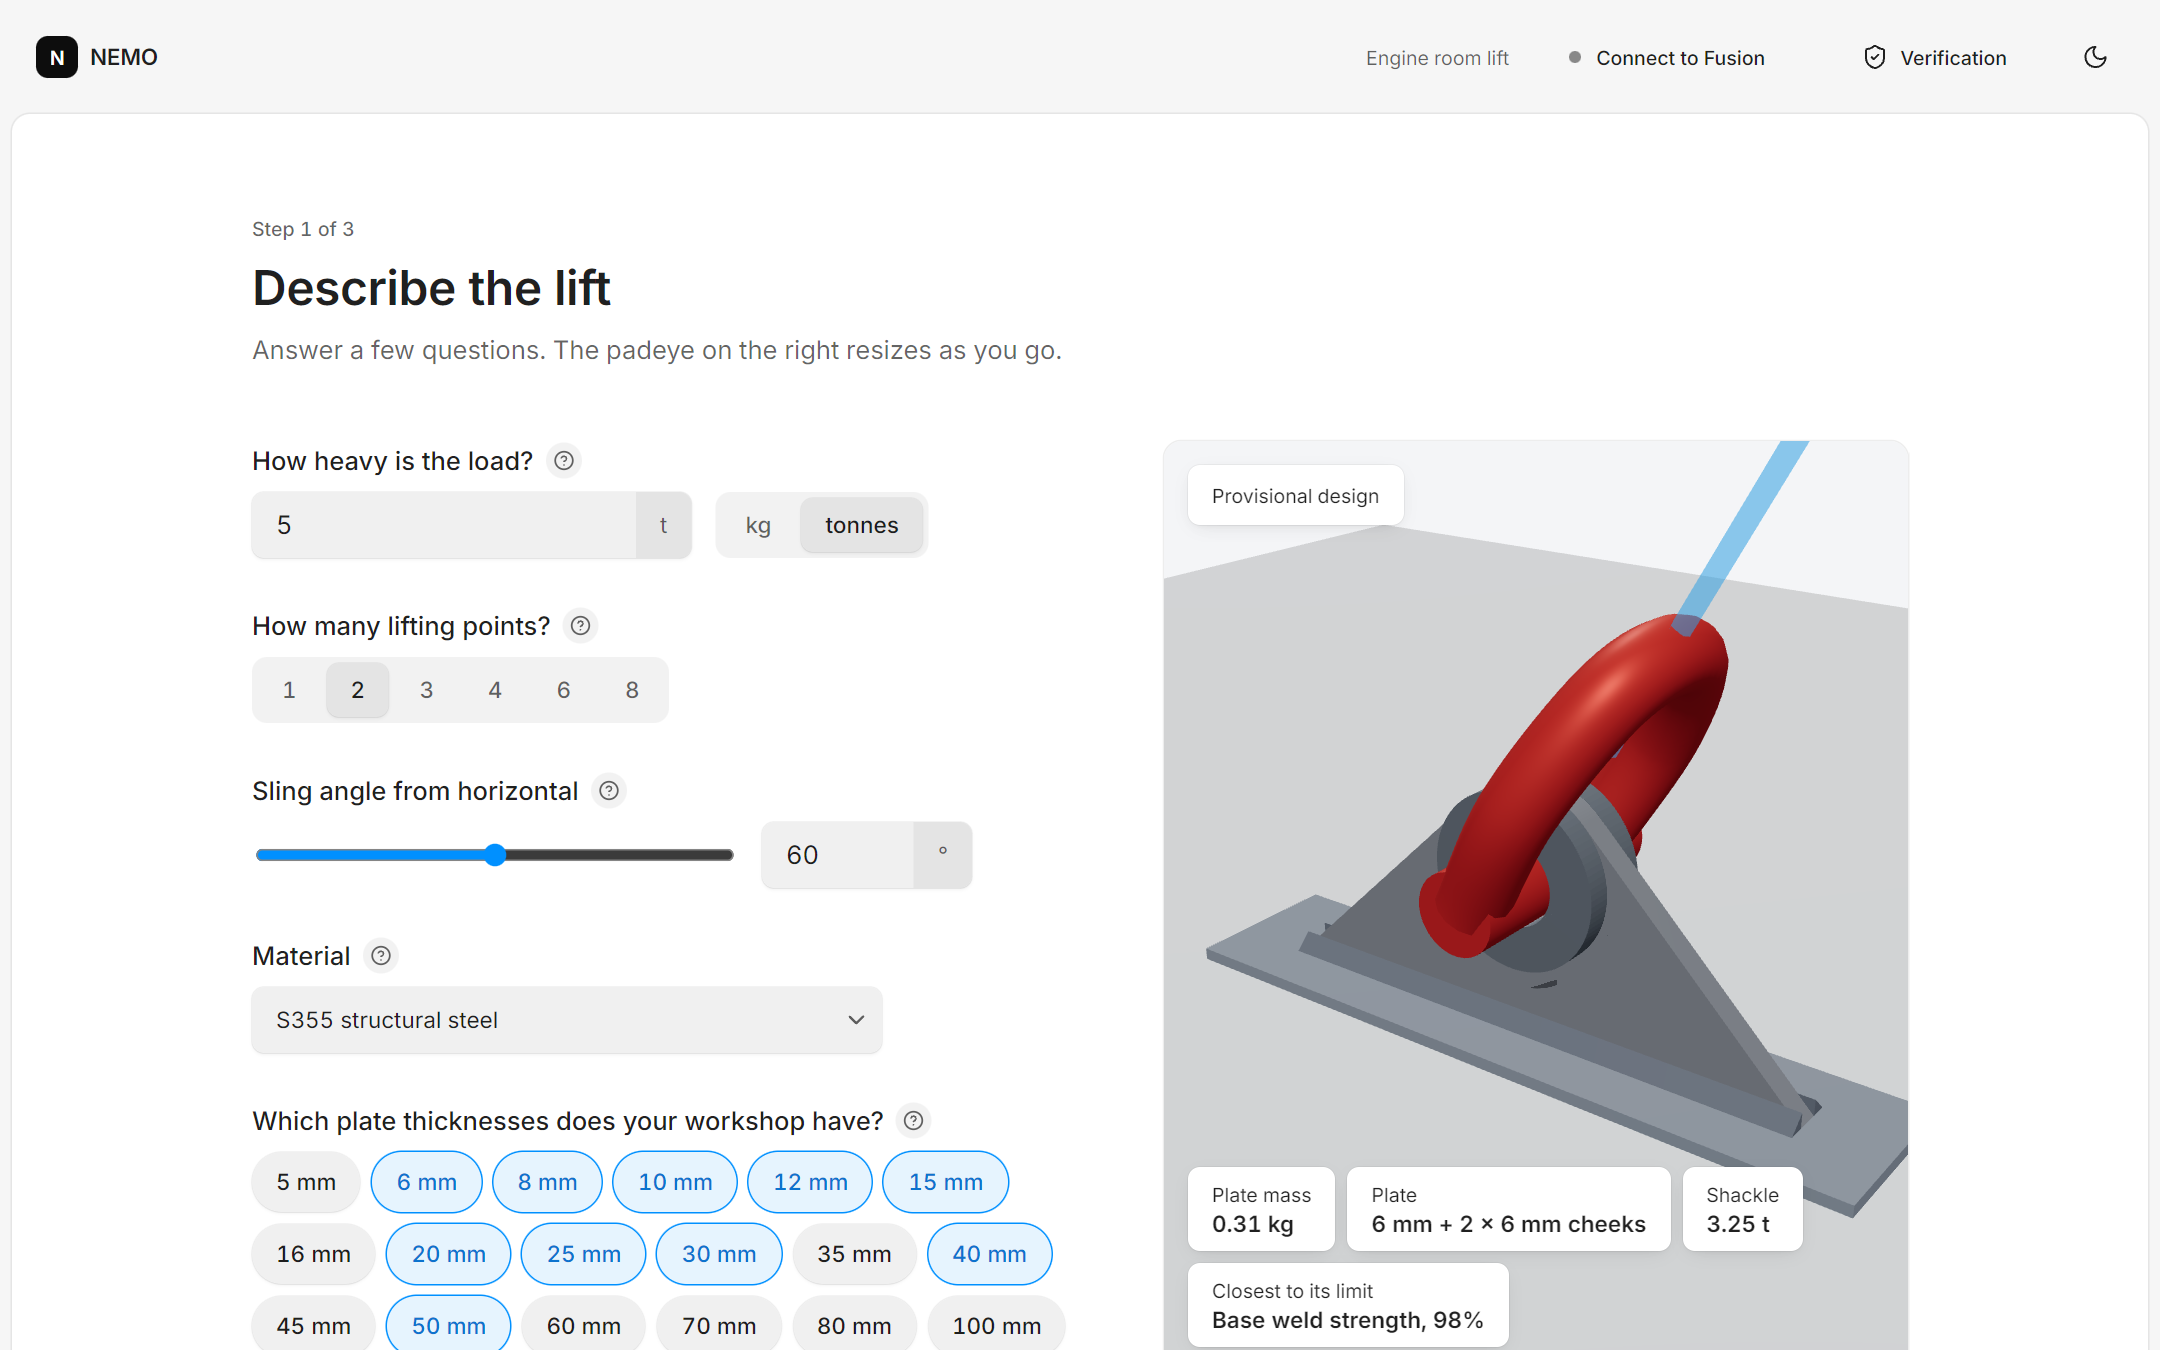
\includegraphics[width=\textwidth]{images/app-padeye-describe.png}
\caption{Job description form for a lifting padeye with the live 3D preview}
\label{fig:app-describe}
\end{figure}

\begin{figure}[H]
\centering
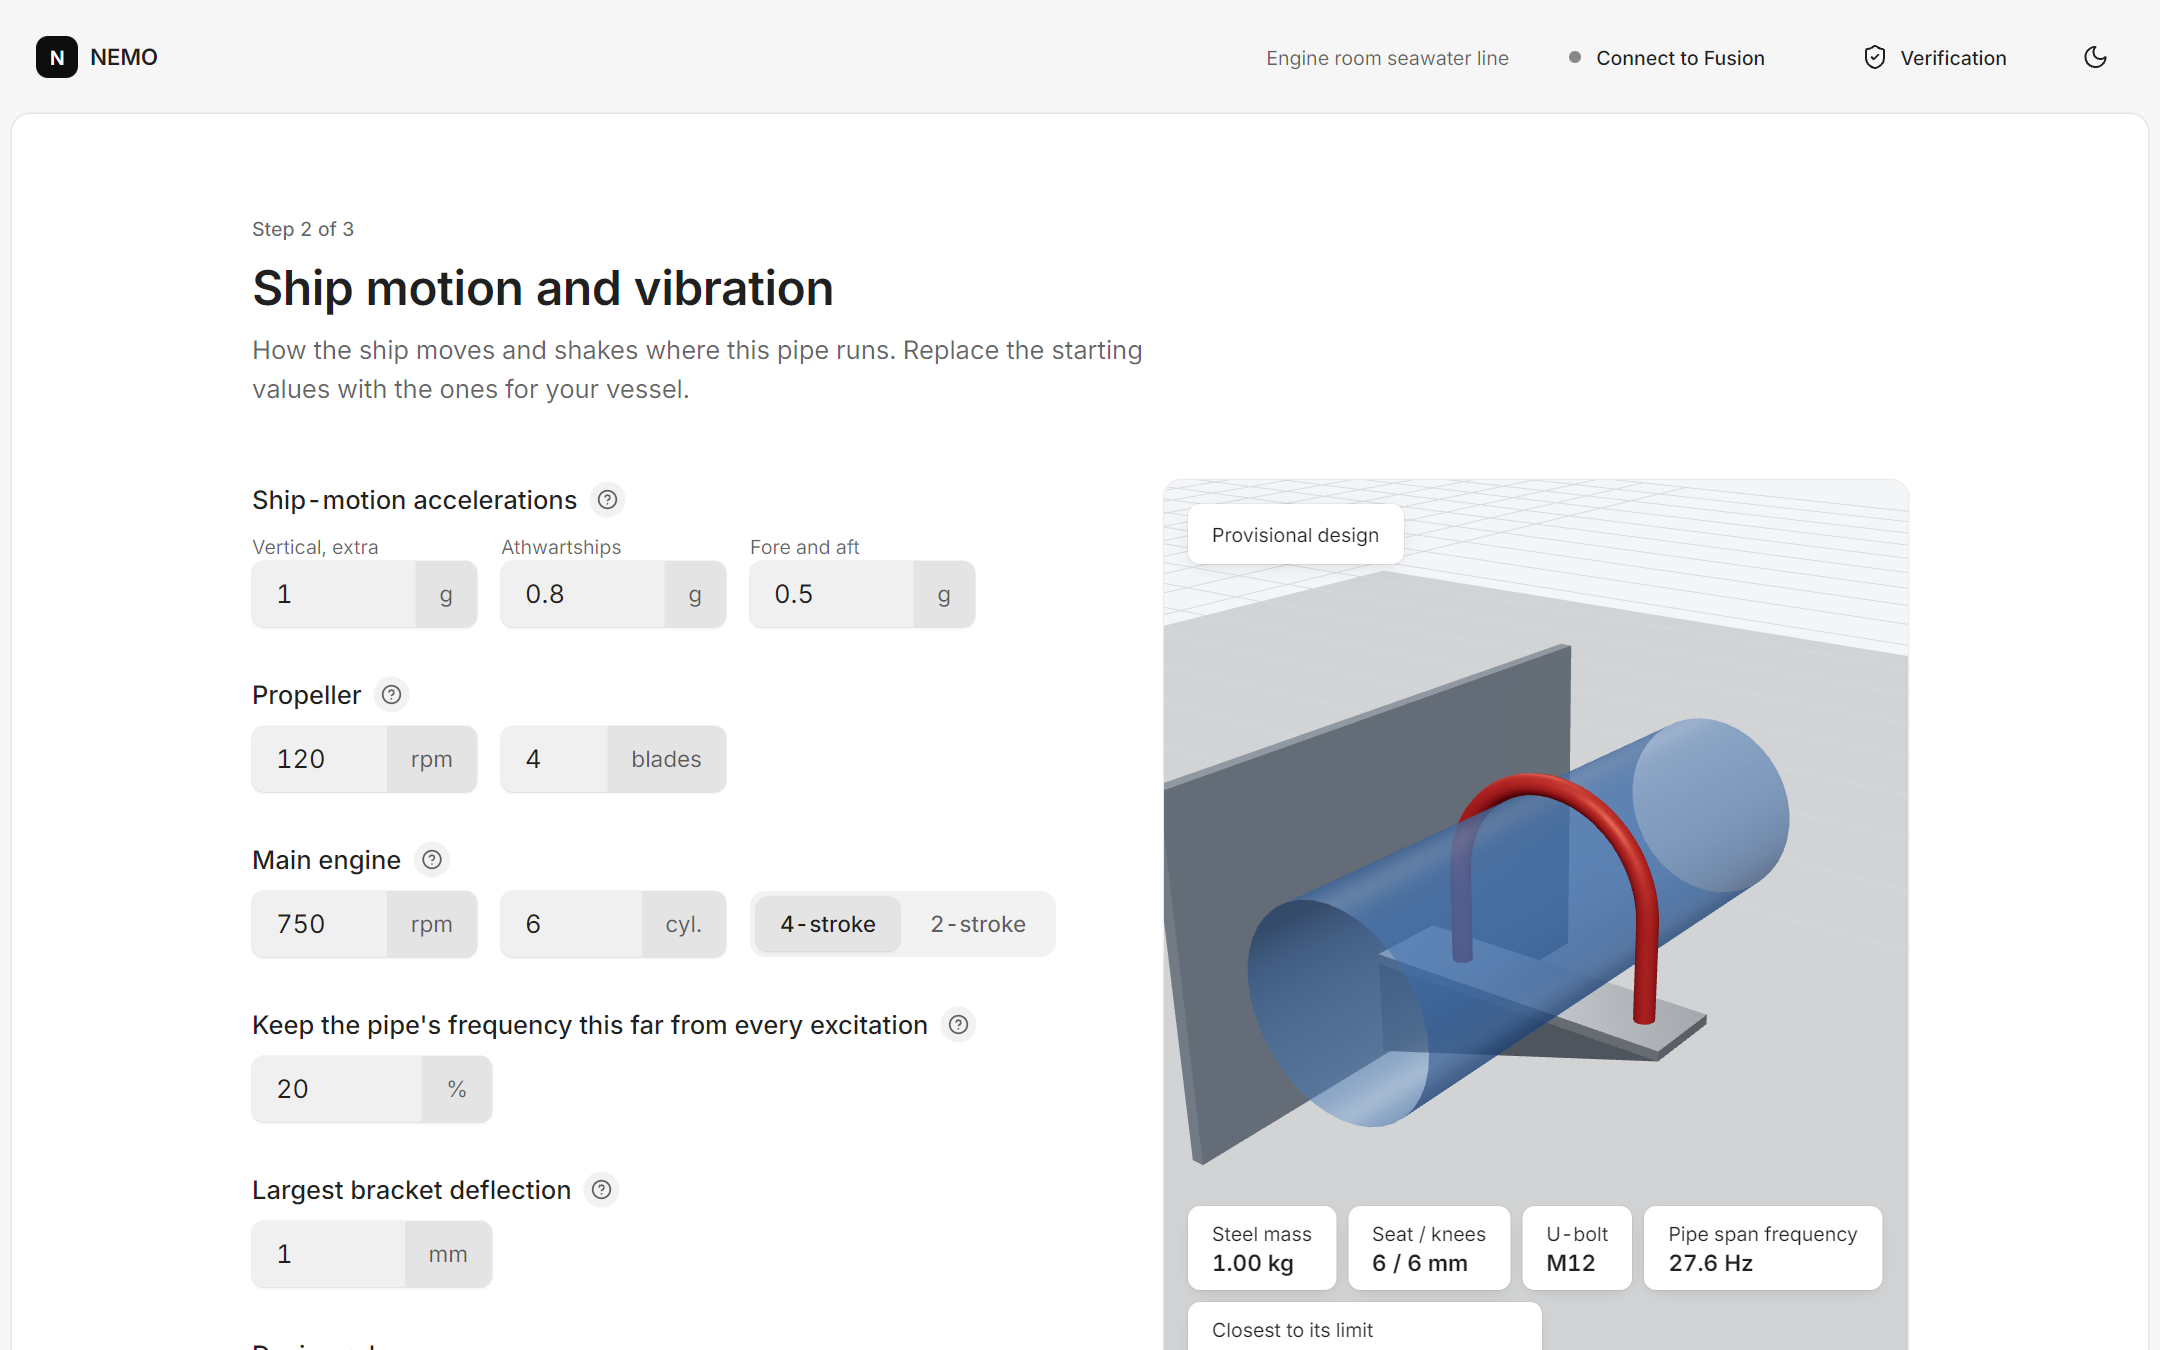
\includegraphics[width=\textwidth]{images/app-bracket-motion.png}
\caption{Ship motion and machinery vibration form for a pipe support bracket}
\label{fig:app-bracket-motion}
\end{figure}

\begin{figure}[H]
\centering
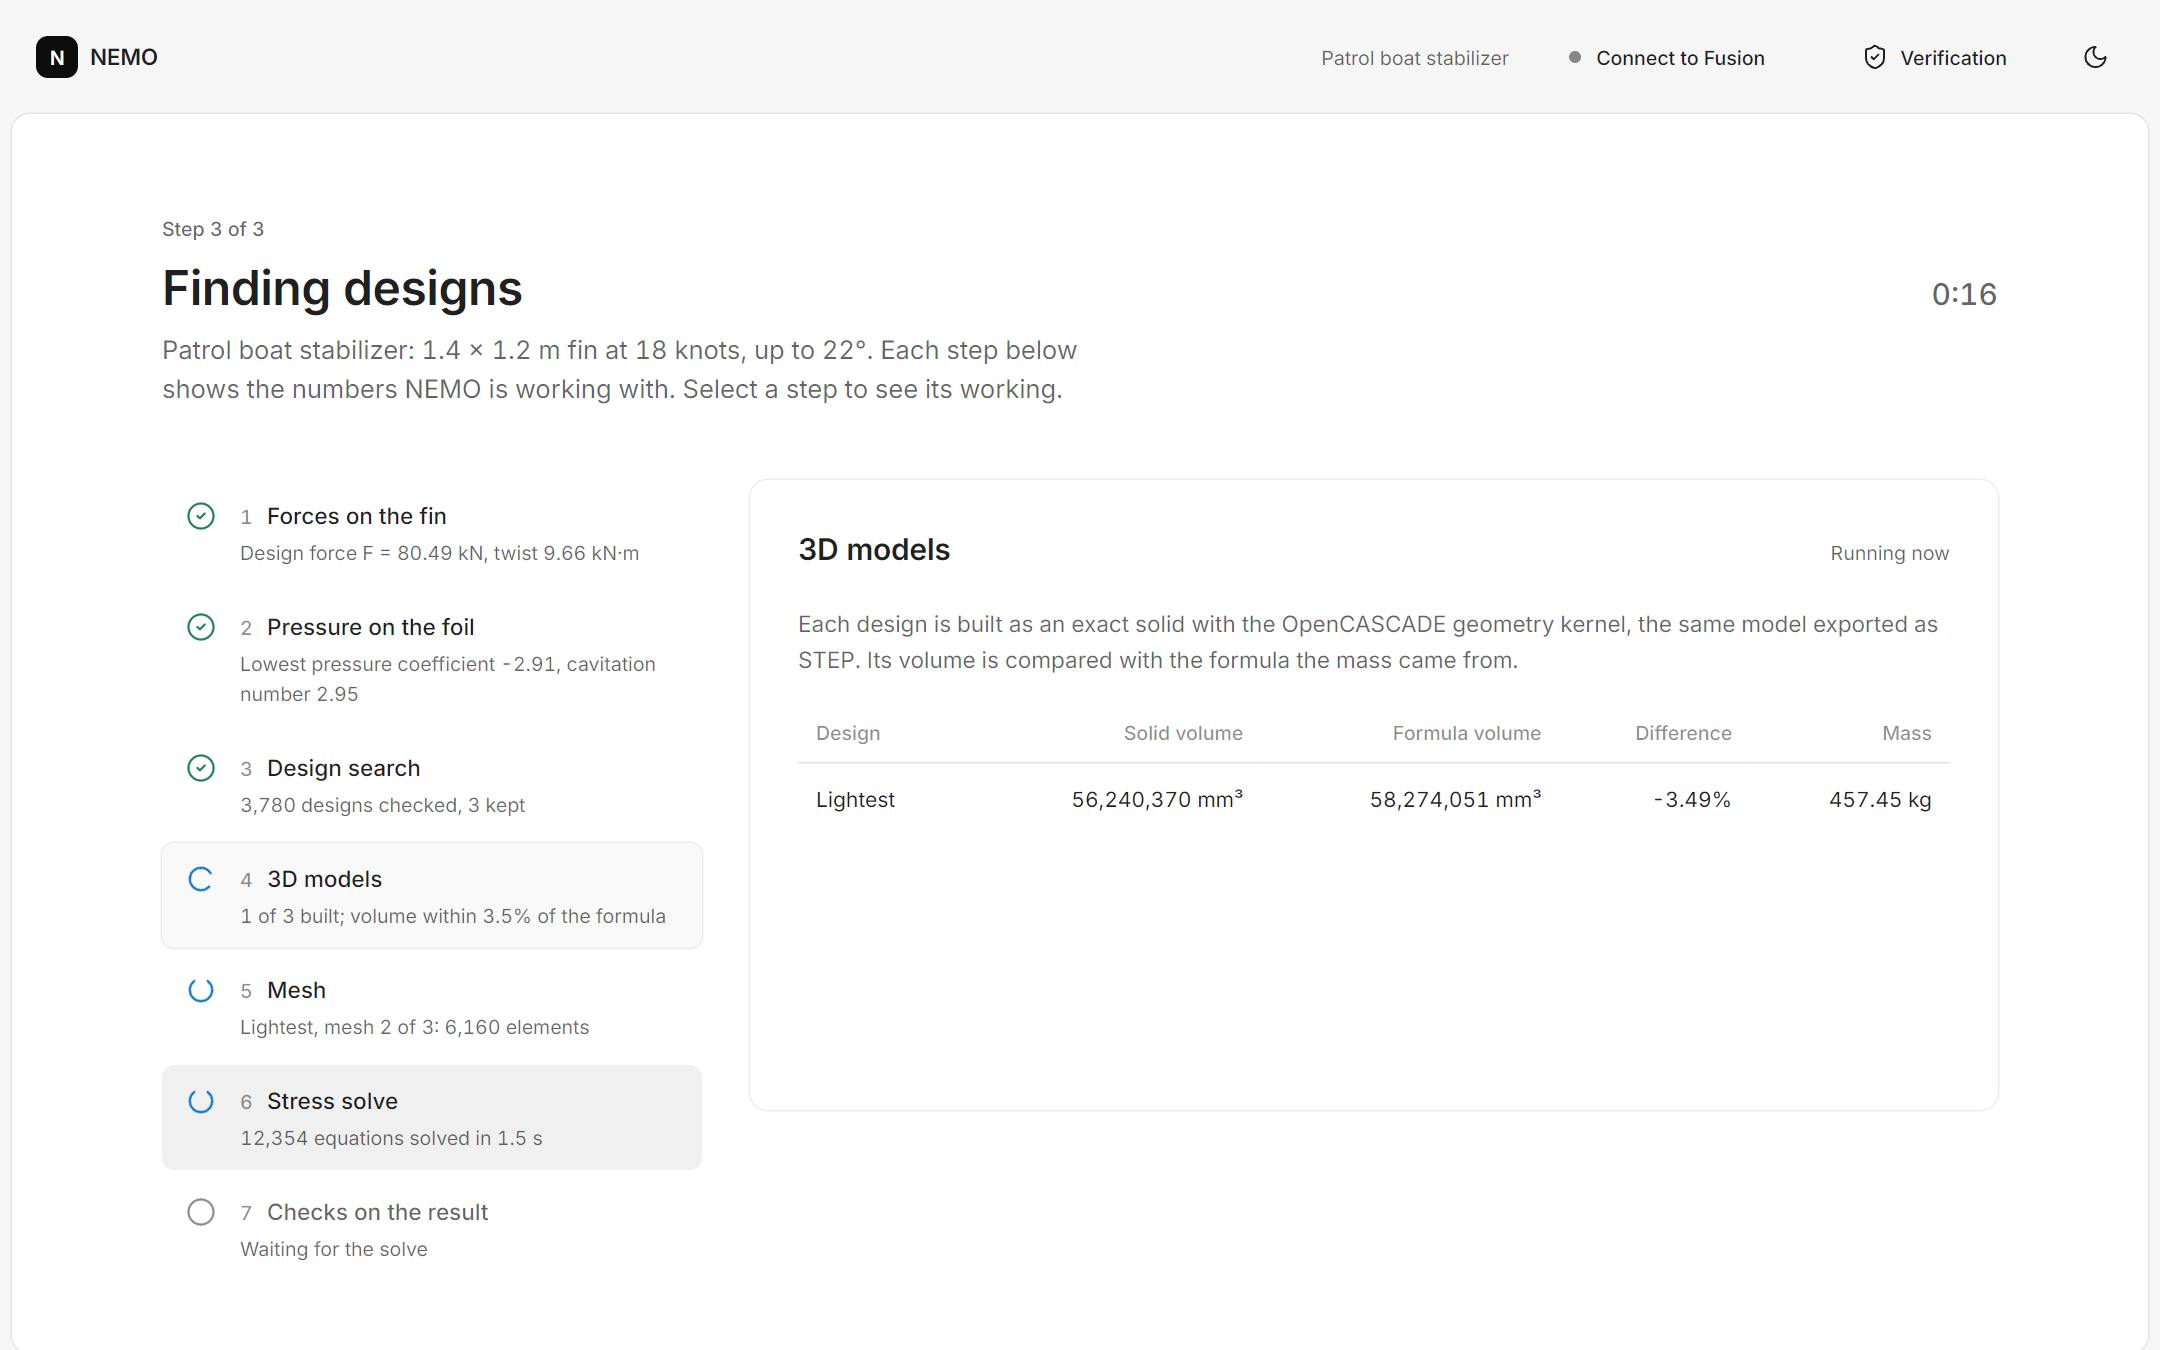
\includegraphics[width=\textwidth]{images/app-running.png}
\caption{Live run screen during the fin case study, with the 3D model step
selected}
\label{fig:app-running}
\end{figure}

\section{Fusion connector}
\label{sec:fusion-connector}

The Fusion connector is an optional add-in for Autodesk Fusion that works with
padeyes. Rather than writing persistent request files that can rebuild stale
geometry on startup, it polls the local \NEMO{} server over HTTP every 1.5~s. A
job that is not picked up within 45~s, or not finished within 180~s, expires,
and each job is handed out only once, which answers requirement R8.

When the user sends a design to Fusion, the add-in builds a parametric model.
The dimensions are user parameters named \code{nemo\_t}, \code{nemo\_R},
\code{nemo\_Dh}, \code{nemo\_L}, \code{nemo\_h}, \code{nemo\_tc} and
\code{nemo\_Rc}, bound to the sketch dimensions and extrusions, so the design
can be edited in Fusion's parameter table. The add-in assigns the material,
names the hole and base faces, and reports Fusion's volume back to \NEMO{} for
comparison with its own. Fusion's material library holds American AISI and
ASTM grades but none of the EN or IACS grades \NEMO{} uses, and its generic
\emph{Steel} has a yield strength of 207~MPa. The add-in (version 1.1.1)
therefore copies \emph{Steel} into the design, names the copy after the
\NEMO{} grade, converts and assigns its modulus, Poisson's ratio, density,
yield and ultimate strength (guarding against Fusion's negative unit-conversion
error sentinel and empty property units), and reads every value back. \NEMO{}
records whether they match, and the cross-check sheet gives manual steps if
they do not. A \emph{Check in NEMO} command sends edited parameters back, and
\NEMO{} re-runs every check and displays the results inside Fusion.

Fusion's API cannot create or solve a Simulation study \cite{autodeskAddins},
so a Fusion stress cross-check is set up by hand using a sheet that \NEMO{}
generates with the loads, supports and material. The engineer enters Fusion's
total reaction and peak stress, and \NEMO{} counts the two analyses as agreeing
when the reaction is within 2\% of the applied load and the peak stress near
the hole is within 15\% of \NEMO{}'s. A reaction less than half or more than
1.5 times the applied load is refused and not recorded: a fixed support always
carries the whole load, so such a value can only have been read from the wrong
result. The sheet lists the three-dimensional resultant and all three load
components, specifies both a global mesh size and a local hole mesh size, and
warns the engineer to probe on the inner pin-hole surface rather than reading
the legend maximum at the fixed base corners or at an unmodeled 90$^\circ$
cheek-plate step. The record is added to section~7 of the PDF. The server side
of the connector, including the job queue, job expiry, unit-conversion guards
and the material record, is covered by the automated tests.
Section~\ref{sec:fusion-session} reports the initial Fusion cross-check trial.

The connector builds padeyes only. For brackets and fins, section~8 of their
calculation packages lists the same values for a cross-check by hand from the
STEP file, including the material values, the load face to split off and the
fin's twisting moment. For the fin it uses \code{fin-stock.step}, because
\NEMO{}'s stress check models the stock alone.

\section{Case studies}
\label{sec:case-studies}

One case per part was chosen to be typical of work in a small yard or an
engine room refit. Table~\ref{tab:cases} gives the inputs. All three were run
with the default plate stock of the material and the default settings
otherwise. For the advanced settings this means a padeye lined up with its
sling ($\beta = 0^\circ$), the bracket's flexibility included, the fin's
astern condition included at the rule's least astern speed of 9~knots, and the
fin's bearing check off. Section~\ref{sec:advanced-results} then uses the
advanced settings on the same cases. The results are in
Chapter~\ref{chap:results}.

\begin{table}[H]
\centering
\caption{Case-study inputs}
\label{tab:cases}
\small
\begin{tabularx}{\textwidth}{>{\raggedright\arraybackslash}p{0.17\textwidth}>{\raggedright\arraybackslash}X}
\toprule
\textbf{Case} & \textbf{Inputs}\\
\midrule
Engine room lift (padeye) & 5~t lifted on two padeyes, sling angle 60$^\circ$, dynamic factor 1.0, sideways allowance 5\%, S355 plate from 6~mm to 50~mm, cheek plates allowed, BTH-1 design category~B, service class~0, E70XX electrodes\\
Engine room seawater line (bracket) & NPS~4 STD carbon steel pipe full of sea water, no insulation, 3~m spacing, continuity factor 1.25, fore-and-aft pipe, accelerations 1.0~g vertical, 0.8~g athwartships and 0.5~g fore-and-aft, friction 0.3, 50~mm gap to the bulkhead, Grade~A plate from 6~mm to 20~mm, class 4.6 U-bolt, propeller 120~rpm with 4 blades, six-cylinder four-stroke engine at 750~rpm, 20\% frequency margin, 1~mm deflection limit\\
Patrol boat stabilizer (fin) & 1.4~m span, 1.2~m chord, NACA~0020, 18~knots, largest angle 22$^\circ$, stock at 35\% chord, spars at 15\% and 65\% chord, fin 3~m below the surface, draught 5~m, 200~mm root-to-bearing gap, AH36 plate from 8~mm to 25~mm, 42CrMo4 stock, 10~mm tip deflection limit\\
\bottomrule
\end{tabularx}
\end{table}

Parameter sweeps were run on the same cases to see how the designs respond.
The padeye was sized for loads of 1~t to 40~t at sling angles of 45$^\circ$,
60$^\circ$ and 90$^\circ$. The bracket was run for pipe sizes NPS~2 to NPS~12,
and its pipe span for spacings of 1.5~m to 6~m. The fin was sized for speeds
of 10 to 24~knots. The data and scripts that produce every figure and number
in Chapter~\ref{chap:results} are kept with this report, in \code{data/} and
\code{tools/}, so the results can be regenerated.

\chapter{Results and discussion}
\label{chap:results}

This chapter presents what the tool produced and how far its results can be
trusted. It starts with the verification results, because the case studies
depend on them. It then gives the three case studies, each with its designs,
checks, finite element results and parameter sweeps. The later sections show
the calculation package and the application, report run times, compare the
two phases of the project and answer the research questions. All numbers come
from the runs kept in \code{data/} with this report.

\section{Verification results}
\label{sec:verification-results}

The full benchmark suite ran in 27.9~s and every comparison passed its
tolerance. Table~\ref{tab:verification} lists the results and
Figure~\ref{fig:verification} plots each error against its tolerance on a log
scale.

\begin{table}[H]
\centering
\caption{Verification results}
\label{tab:verification}
\small
\begin{tabularx}{\textwidth}{>{\raggedright\arraybackslash}Xrrrr}
\toprule
\textbf{Quantity} & \textbf{Reference} & \textbf{\NEMO{}} & \textbf{Error} & \textbf{Tolerance}\\
\midrule
\multicolumn{5}{l}{\emph{Padeye hand calculation, 4~t on two points at 60$^\circ$, S355, 20~mm plate}}\\
Sling force $F$ (N) & 22,647.6 & 22,647.5 & $-0.0005\%$ & 0.1\%\\
Strength reduction $C_r$ & 0.885696 & 0.885696 & $0.0000\%$ & 0.1\%\\
Effective width $b_\text{eff}$ (mm) & 22.0013 & 22.0013 & $+0.0002\%$ & 0.1\%\\
Tension through pinhole $P_t$ (N) & 101,763 & 101,763 & $-0.0002\%$ & 0.1\%\\
Fracture beyond pinhole $P_b$ (N) & 117,933 & 117,933 & $0.0000\%$ & 0.1\%\\
Shear plane area $A_v$ (mm$^2$) & 1,492.61 & 1,492.61 & $+0.0003\%$ & 0.1\%\\
Double plane shear $P_v$ (N) & 136,408 & 136,408 & $+0.0003\%$ & 0.1\%\\
Pin bearing $P_p$ (N) & 54,912.5 & 54,912.5 & $0.0000\%$ & 0.1\%\\
Base combined use & 0.14898 & 0.148982 & $+0.0016\%$ & 0.1\%\\
Base weld stress (MPa) & 26.179 & 26.1788 & $-0.0008\%$ & 0.1\%\\
Plate mass (kg) & 2.5958 & 2.59578 & $-0.0006\%$ & 0.1\%\\
\midrule
\multicolumn{5}{l}{\emph{CAD volume against the exact formula}}\\
Plain padeye (mm$^3$) & 330,673 & 330,673 & $0.0000\%$ & 0.01\%\\
Padeye with cheek plates (mm$^3$) & 424,000 & 424,000 & $0.0000\%$ & 0.01\%\\
Pipe support bracket (mm$^3$) & 324,921 & 324,921 & $0.0000\%$ & 0.01\%\\
\midrule
\multicolumn{5}{l}{\emph{Cantilever, 3,487 elements, 19,479 equations}}\\
Tip deflection (mm) & 0.95981 & 0.95216 & $-0.80\%$ & 3\%\\
Bending stress at mid-span (MPa) & 75.0 & 76.97 & $+2.63\%$ & 4\%\\
\midrule
\multicolumn{5}{l}{\emph{Plate with a hole, 16,749 elements, 96,000 equations}}\\
Stress concentration factor & 3.0322 & 3.0597 & $+0.91\%$ & 5\%\\
\midrule
\multicolumn{5}{l}{\emph{Panel method}}\\
Lowest $C_p$ on a circle & $-3.000$ & $-2.998$ & $-0.05\%$ & 0.5\%\\
NACA 0012 lift slope (per rad) & 6.864 & 6.939 & $+1.09\%$ & 3\%\\
NACA 0020 lift slope (per rad) & 7.251 & 7.370 & $+1.65\%$ & 3\%\\
\midrule
\multicolumn{5}{l}{\emph{Fin stock, 6,160 elements, 31,584 equations}}\\
Equivalent stress near the bearing (MPa) & 165.67 & 165.46 & $-0.13\%$ & 4\%\\
\midrule
Support reactions, all three finite element models & & & $0.0000\%$ & $10^{-6}\%$\\
\bottomrule
\end{tabularx}
\end{table}

\begin{figure}[H]
\centering
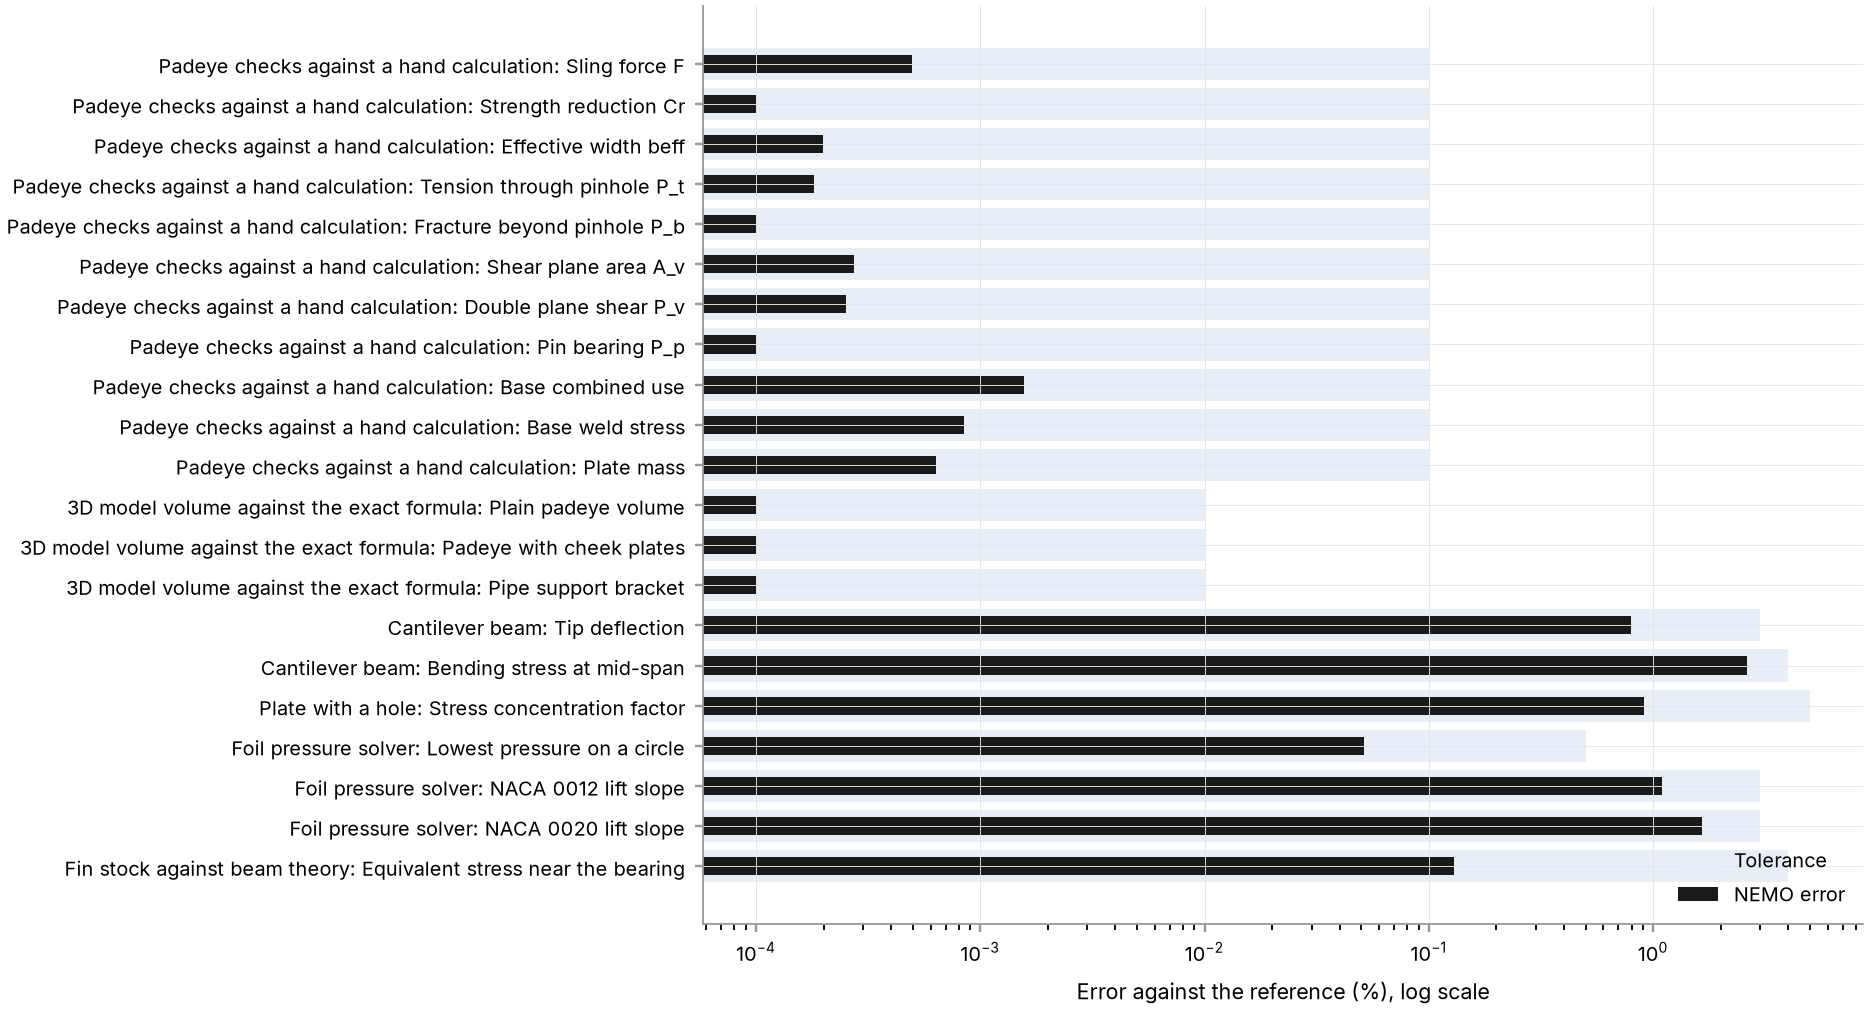
\includegraphics[width=0.95\textwidth]{images/verification.png}
\caption{Error of each verification quantity against its tolerance}
\label{fig:verification}
\end{figure}

The padeye hand calculation agrees to better than 0.002\% in every quantity.
The remaining differences come from rounding in the hand calculation, which
was carried to six significant figures. This confirms that the code
implements the BTH-1 expressions as written in the engineering manual. It
does not confirm that the manual reads BTH-1 correctly. That needs a published
worked example, which has not yet been done.

The CAD volumes match the formulas exactly. The geometry code and the mass
code were written separately, one from the build123d solid and one from the
analytic outline, so this agreement checks both.

The finite element errors are small and have the expected signs. The
cantilever tip deflection is 0.8\% low, which is consistent with the slight
stiffness of a coarse quadratic mesh. The mid-span bending stress is 2.6\%
high, inside its 4\% tolerance. The finite element value is a von Mises
stress averaged at mesh vertices, while beam theory gives the axial stress
alone. The two are not quite the same quantity, and a difference of a few per
cent is expected at this mesh density. The stress concentration factor of the
plate with a hole is
0.9\% above Heywood's value \cite{peterson2008}. The fin stock agrees with beam
and torsion theory to 0.13\%.

Figure~\ref{fig:panel-validation} shows the panel method results. On a
circle, where the exact pressure is $C_p = 1 - 4\sin^2\theta$, the 160-panel
solution is indistinguishable from the exact curve. The section lift slopes
lie 1\% to 2\% above the thick-section estimate $2\pi(1 + 0.77t/c)$
\cite{abbott1959}. That estimate is itself an approximation and an inviscid
method is expected to sit slightly high, so this is a reasonable result.
Measured slopes for real sections are lower again because of the boundary
layer, which is one reason the fin load does not use the panel method for its
force.

\begin{figure}[H]
\centering
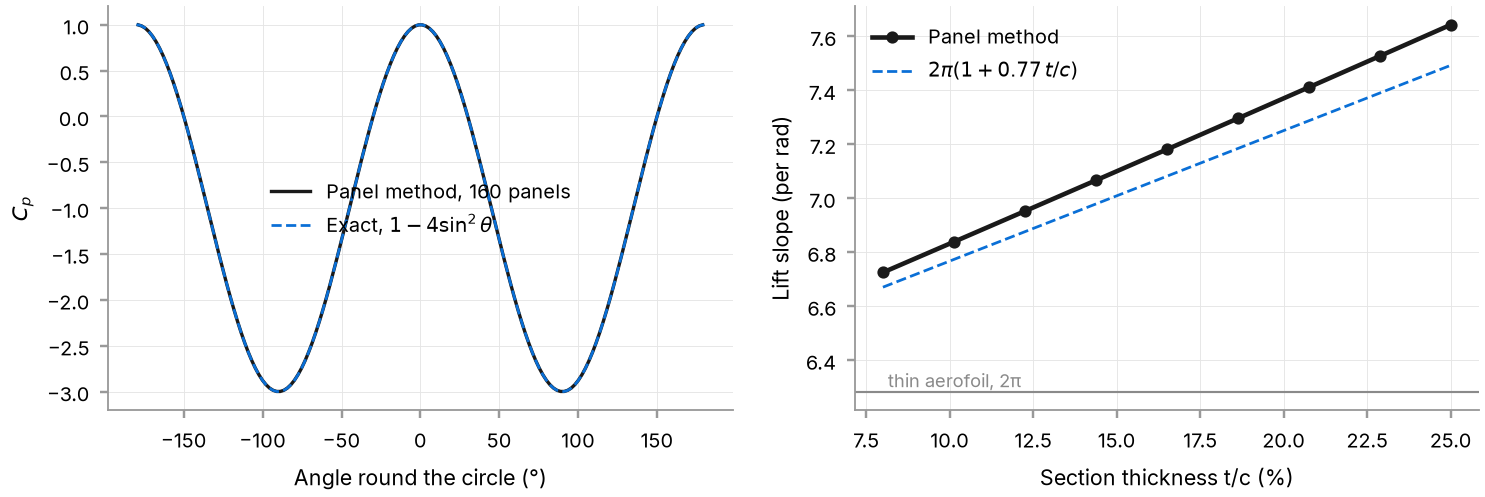
\includegraphics[width=0.95\textwidth]{images/panel-validation.png}
\caption{Panel method against the exact flow round a circle and the
thick-section lift slope}
\label{fig:panel-validation}
\end{figure}

All 153 automated tests passed on the final version of the engine. The
benchmarks can also be run from the application (Figure~\ref{fig:app-verification}).

\begin{figure}[H]
\centering
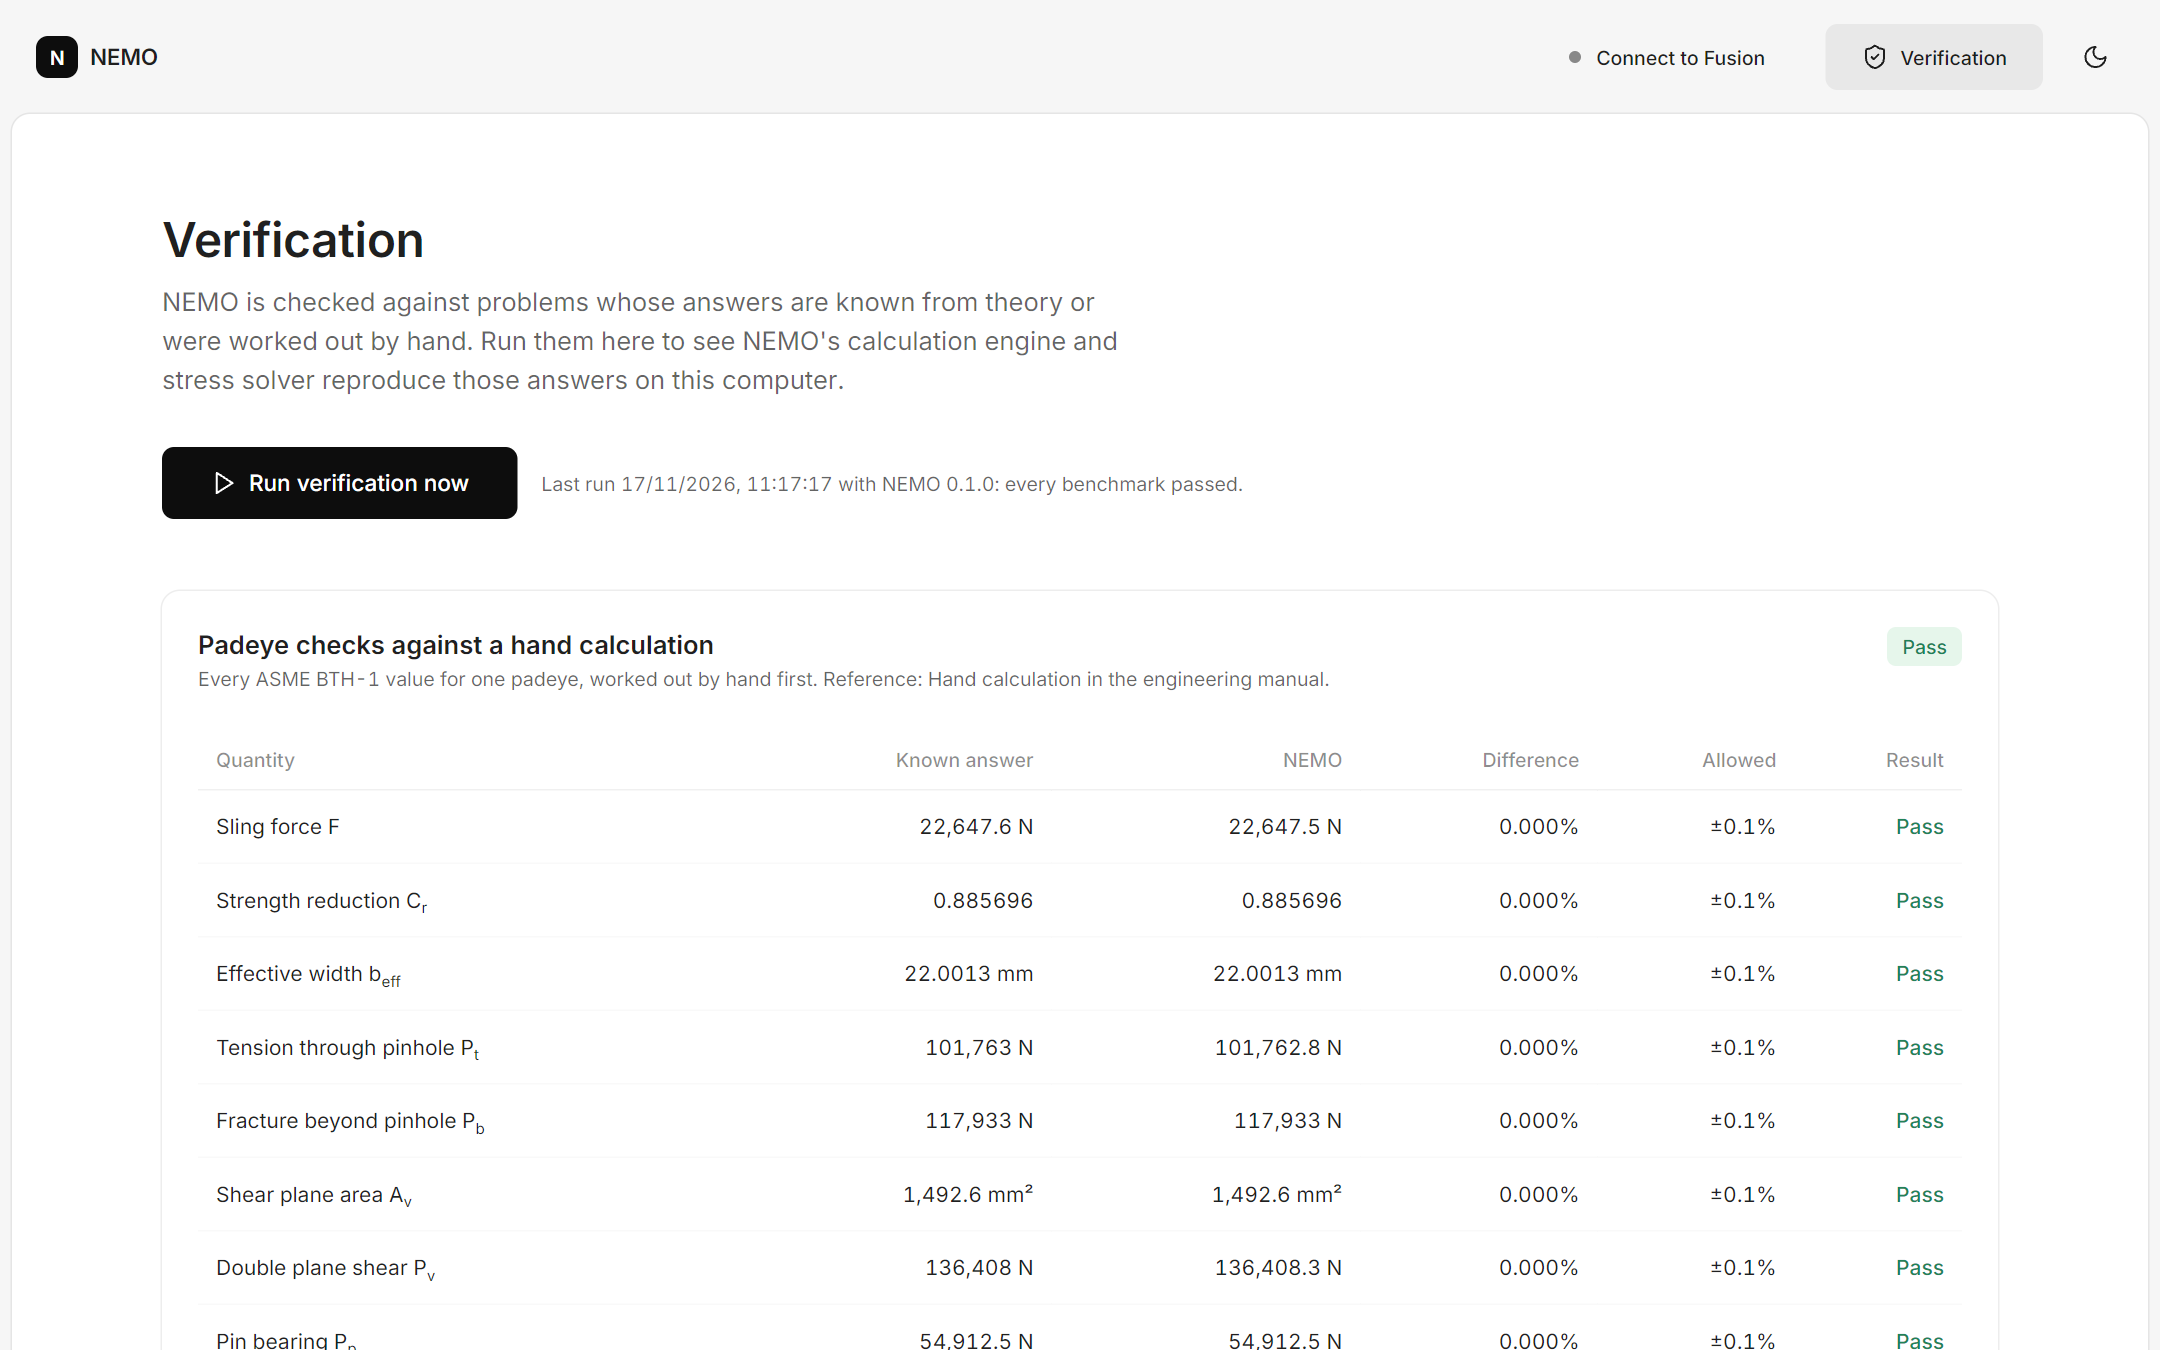
\includegraphics[width=0.8\textwidth]{images/app-verification.png}
\caption{Verification page of the application after a run}
\label{fig:app-verification}
\end{figure}

\section{Case study 1: engine room lift padeye}
\label{sec:padeye-results}

\subsection{Loads}

A 5~t load lifted on two padeyes with slings at 60$^\circ$ gives, from
Equation~\eqref{eq:padeye-loads}, $W = 49.03$~kN, $V = 24.52$~kN per padeye
and a sling force $F = 28.31$~kN, or 2.887~t. The in-plane horizontal part is
$H = 14.15$~kN and the sideways allowance $Q = 1.415$~kN. The smallest shackle
rated for 2.887~t is the 3.25~t Crosby G-2130, with a 19.1~mm pin and a
26.9~mm jaw.

\subsection{Designs}

The search tried 36 combinations of shackle, plate and cheek thickness across
the three targets and evaluated 19,389 designs. Table~\ref{tab:padeye-designs}
gives the three designs it kept and Figure~\ref{fig:padeye-model} shows the
lightest.

\begin{table}[H]
\centering
\caption{Padeye designs for the 5~t engine room lift}
\label{tab:padeye-designs}
\small
\begin{tabularx}{\textwidth}{Xrrr}
\toprule
& \textbf{Lightest} & \textbf{Balanced} & \textbf{Extra margin}\\
\midrule
Target maximum use & 100\% & 85\% & 70\%\\
Shackle (Crosby G-2130) & 3.25~t & 4.75~t & 4.75~t\\
Main plate (mm) & 6 & 8 & 8\\
Cheek plates (mm) & $2 \times 6$ & $2 \times 6$ & $2 \times 6$\\
Head radius $R$ (mm) & 21 & 25 & 22\\
Cheek radius $R_c$ (mm) & 21 & 22 & 22\\
Hole diameter $D_h$ (mm) & 20.5 & 23.5 & 23.5\\
Hole height $h$ (mm) & 39 & 45 & 45\\
Base length $L$ (mm) & 140 & 140 & 160\\
Base weld leg (mm) & 4 & 5 & 5\\
Cheek weld leg (mm) & 3 & 5 & 5\\
Steel mass (kg) & 0.305 & 0.432 & 0.447\\
Governing check & Base weld, 98.0\% & Base weld, 81.0\% & Base weld, 67.3\%\\
FEA peak von Mises (MPa) & 228.1 & 189.6 & 200.4\\
Factor of safety on yield & 1.56 & 1.87 & 1.77\\
\bottomrule
\end{tabularx}
\end{table}

The balanced design is 42\% heavier than the lightest, though its target is
only 15 points lower. The jump comes from the shackle. The shackle rating is a
strength check, and the 3.25~t shackle runs at 88.8\% of its working load
limit. That is above the 85\% target, so the balanced design has to move to
the 4.75~t shackle. The larger pin, 22.4~mm, needs a 23.5~mm hole, a wider
jaw fill and a taller head, and the plate goes from 6~mm to 8~mm to fill the
31.8~mm jaw. The extra margin design then costs only 15~g more. This shows how
discrete catalogue steps, not the continuous dimensions, set the mass of small
lifting details.

Table~\ref{tab:padeye-checks} lists every check on the lightest design. The
base weld governs at 98.0\%, followed by the shackle rating at 88.8\% and the
combined stress at the base at 88.1\%. The head checks are between 56\% and
72\%. The cheek plates were chosen because they let a 6~mm main plate fill the
jaw and carry the pin bearing. Without them, the main plate would have to be
thick enough on its own, and a thicker plate is heavier along its whole base.

\begin{table}[H]
\centering
\caption{Checks on the lightest padeye}
\label{tab:padeye-checks}
\small
\begin{tabularx}{\textwidth}{>{\raggedright\arraybackslash}Xrrlr>{\raggedright\arraybackslash}p{0.24\textwidth}}
\toprule
\textbf{Check} & \textbf{Demand} & \textbf{Capacity} & \textbf{Unit} & \textbf{Use} & \textbf{Basis}\\
\midrule
Tearing across the sides of the hole & 28,309 & 45,478 & N & 62.2\% & BTH-1\\
Splitting above the hole & 28,309 & 39,419 & N & 71.8\% & BTH-1\\
Shearing out above the hole & 28,309 & 42,628 & N & 66.4\% & BTH-1\\
Crushing under the shackle pin & 28,309 & 50,854 & N & 55.7\% & BTH-1\\
Pulling and bending at the base & 0.881 & 1 & ratio & 88.1\% & BTH-1\\
Shear at the base & 16.9 & 68.3 & MPa & 24.8\% & BTH-1\\
Base weld strength & 78.7 & 80.3 & MPa & 98.0\% & BTH-1\\
Cheek plate welds & 33.7 & 80.3 & MPa & 42.0\% & BTH-1\\
Shackle is rated for the load & 2.887 & 3.25 & t & 88.8\% & Crosby WLL\\
Hole is big enough for the pin & 20.1 & 20.5 & mm & 98.0\% & Practice\\
Padeye fits inside the shackle & 20 & 26.9 & mm & 74.3\% & Practice\\
Pin fits the hole closely (advice) & 0.90 & 0.932 & ratio & 96.6\% & BTH-1 commentary\\
Padeye fills the shackle jaw (advice) & 16.1 & 18 & mm & 89.7\% & Practice\\
Base weld size (advice) & 3 & 4 & mm & 75.0\% & AWS D1.1\\
Cheek weld size (advice) & 3 & 3 & mm & 100.0\% & AWS D1.1\\
\bottomrule
\end{tabularx}
\end{table}

Figure~\ref{fig:padeye-search} shows every design the search tried for the
lightest target, by mass and highest use. Most of the designs tried pass. None
has a highest use below 88.8\%, the use of the 3.25~t shackle, which no change
to the plate can lower. The designs that fail are the lightest ones, above the
100\% line, and the chosen design sits at the left end of the passing set.

\begin{figure}[H]
\centering
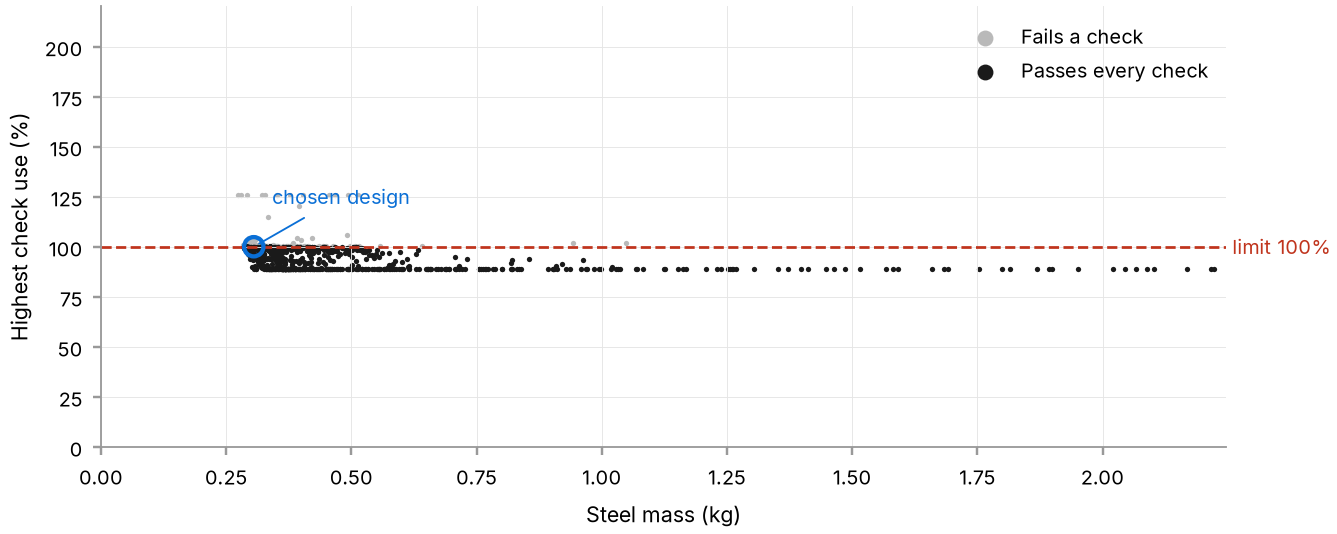
\includegraphics[width=0.75\textwidth]{images/padeye-search.png}
\caption{Designs tried by the search for the lightest padeye}
\label{fig:padeye-search}
\end{figure}

\subsection{Finite element results}

Figure~\ref{fig:padeye-stress} shows the von Mises stress in the lightest
padeye. The highest stress is at the sides of the hole, where the pin load
spreads round the head, as the BTH-1 tension and fracture checks assume.
Table~\ref{tab:padeye-fea} gives the three meshes. The peak in the head
region changed by 0.20\% between the two finest meshes, well inside the 5\%
criterion. The applied load matched the design forces, 14,155~N, 1,415~N and
24,516~N in the three directions, and the force balance error was below
$10^{-12}$ on every mesh.

\begin{figure}[H]
\centering
\begin{subfigure}{0.49\textwidth}
\centering
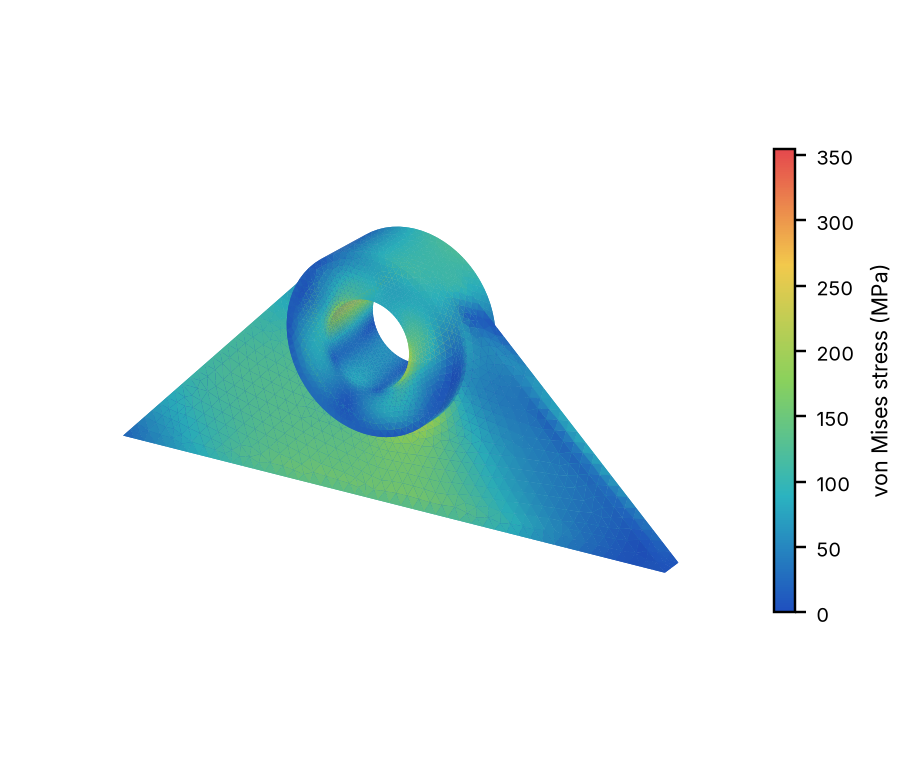
\includegraphics[width=\textwidth]{images/padeye-stress.png}
\caption{Whole padeye}
\end{subfigure}
\hfill
\begin{subfigure}{0.49\textwidth}
\centering
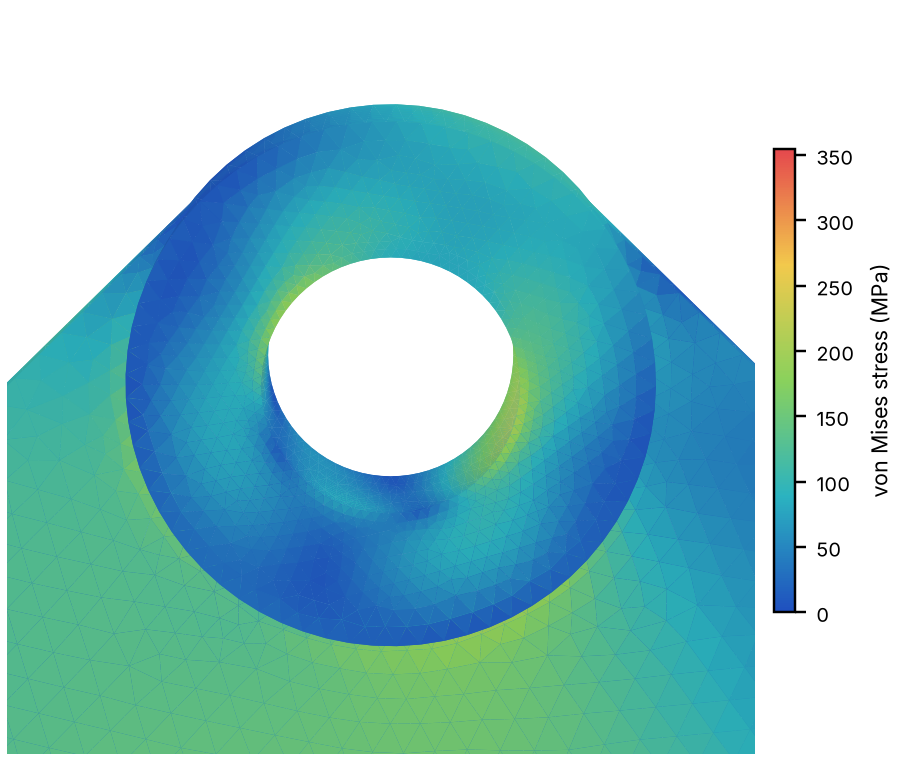
\includegraphics[width=\textwidth]{images/padeye-stress-head.png}
\caption{Head and hole}
\end{subfigure}
\caption{Von Mises stress in the lightest padeye under the 28.3~kN sling force}
\label{fig:padeye-stress}
\end{figure}

\begin{table}[H]
\centering
\caption{Mesh study of the lightest padeye}
\label{tab:padeye-fea}
\small
\begin{tabular}{lrrr}
\toprule
& \textbf{Mesh 1} & \textbf{Mesh 2} & \textbf{Mesh 3}\\
\midrule
Element size, general / at hole (mm) & 6.00 / 1.61 & 4.20 / 1.13 & 3.00 / 0.81\\
Elements & 6,487 & 17,200 & 44,271\\
Unknowns & 34,986 & 86,325 & 209,763\\
Peak von Mises in head region (MPa) & 227.56 & 227.63 & 228.09\\
Largest displacement (mm) & 0.1647 & 0.1662 & 0.1671\\
Force balance error & $1.0\times10^{-12}$ & $4.1\times10^{-13}$ & $2.1\times10^{-13}$\\
Solve time (s) & 4.2 & 12.9 & 26.9\\
\bottomrule
\end{tabular}
\end{table}

The peak of 228~MPa is 64\% of the 355~MPa yield stress, a factor of safety
of 1.56, while the code checks report the design at 98\% use. The two numbers
measure different things and do not conflict. BTH-1 category~B applies a
design factor of 3.0 to strength, and 3.6 to pin-connected plates, so a
design at 100\% use is still far from failure. The finite element peak is an
elastic local stress at the edge of the hole, which includes the stress
concentration that the code capacities allow for through their empirical
coefficients. Its role is to confirm the load path and to show that no part of
the plate yields at the working load. The governing weld is not in the solid
model, because the model treats the plate and deck as joined. The weld check
therefore rests on the hand calculation alone.

\subsection{Response to load and sling angle}

Figure~\ref{fig:padeye-load-sweep} shows the mass of the lightest padeye for
loads of 1~t to 40~t at three sling angles. The mass rises faster than the
load. At 40~t the padeye for 45$^\circ$ slings weighs 7.50~kg, against 5.26~kg
at 60$^\circ$ and 3.34~kg at 90$^\circ$, because a flatter sling raises both
the sling force and the bending at the base.

\begin{figure}[H]
\centering
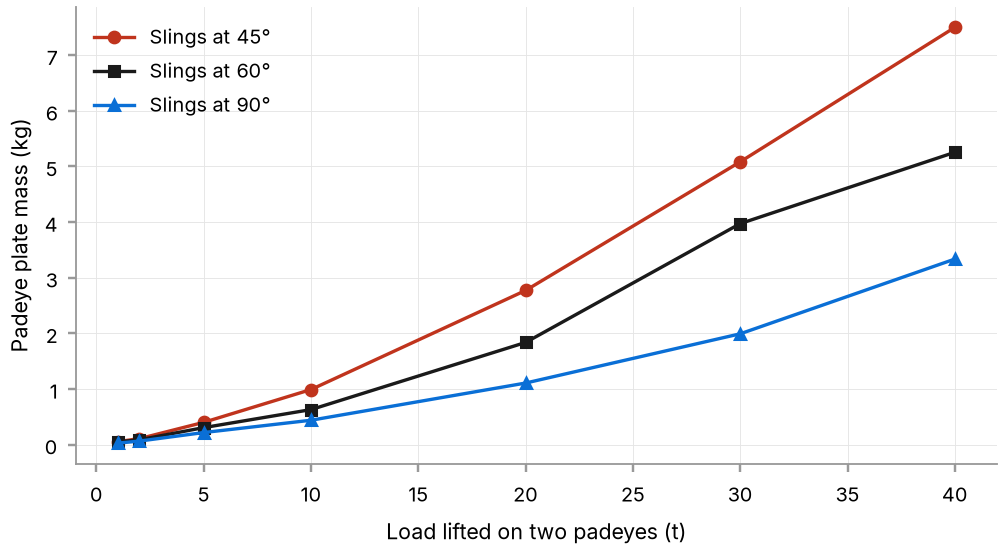
\includegraphics[width=0.75\textwidth]{images/padeye-load-sweep.png}
\caption{Mass of the lightest padeye against the load lifted on two padeyes}
\label{fig:padeye-load-sweep}
\end{figure}

The governing check changes along the sweep. At 1~t and 2~t the base weld
governs, except with vertical slings, where the shackle rating governs at
100\% because the sling force equals the working load limit of a standard
size. At most loads between 5~t and 20~t the base weld or the combined stress
at the base governs. Splitting above the hole governs from 20~t at
45$^\circ$ and from 30~t at 60$^\circ$ and 90$^\circ$, at 96\% to 100\%. It
also governs the 5~t padeye on vertical slings, which uses a 20~mm plate
without cheeks. The curves are not smooth because the plate thickness and the
shackle size change in steps. At 60$^\circ$, for example, the 2~t padeye uses
a 12~mm plate without cheeks and the 5~t padeye a 6~mm plate with cheeks.

\section{Case study 2: engine room seawater line bracket}
\label{sec:bracket-results}

\subsection{Loads}

An NPS~4 standard-wall carbon steel pipe, 114.3~mm by 6.02~mm, weighs
16.08~kg/m, and its sea water adds 8.42~kg/m. The weight per metre is
240.2~N/m. With 3~m spacing and the continuity factor of 1.25, one bracket
carries 0.901~kN. The ship motion raises this to 1.80~kN downward, with
0.72~kN across the pipe and 0.54~kN of friction along it.

\subsection{Design}

The search found one design. The lightest bracket uses so little of its
strength that it already meets the 85\% and 70\% targets, so the other two
searches returned the same design and the tool offered it alone.
Table~\ref{tab:bracket-design} gives the design and
Table~\ref{tab:bracket-checks-result} its checks. The search ran 63
combinations of seat and knee thickness over the three targets. Lower-bound
pruning skipped 60 of them, and only 300 designs had to be evaluated.

\begin{table}[H]
\centering
\caption{Pipe support bracket for the NPS~4 seawater line}
\label{tab:bracket-design}
\small
\begin{tabular}{lr}
\toprule
Seat plate, length by width by thickness (mm) & $195 \times 50 \times 6$\\
Knees, two, thickness (mm) & 6\\
Knee depth at the bulkhead (mm) & 60\\
Pipe centre from the bulkhead (mm) & 107.15\\
U-bolt & M12, class 4.6, galvanised\\
Fillet welds, bulkhead and knee to seat (mm) & 3 and 3\\
Steel mass (kg) & 0.996\\
Governing strength check & Welds to the bulkhead, 25.4\%\\
FEA peak von Mises, away from the bulkhead (MPa) & 34.65\\
Hand stress, seat between the knees (MPa) & 37.53\\
\bottomrule
\end{tabular}
\end{table}

\begin{table}[H]
\centering
\caption{Checks on the bracket and the pipe span}
\label{tab:bracket-checks-result}
\small
\begin{tabularx}{\textwidth}{>{\raggedright\arraybackslash}Xrrlr}
\toprule
\textbf{Check} & \textbf{Demand} & \textbf{Capacity} & \textbf{Unit} & \textbf{Use}\\
\midrule
Bending along the bracket arm & 0.191 & 1 & ratio & 19.1\%\\
Shear in the arm & 2.89 & 84.4 & MPa & 3.4\%\\
Welds to the bulkhead & 36.7 & 144.6 & MPa & 25.4\%\\
Knee-to-seat welds & 3.32 & 144.6 & MPa & 2.3\%\\
Seat plate between the knees & 37.5 & 211.1 & MPa & 17.8\%\\
U-bolt legs & 0.003 & 1 & ratio & 0.3\%\\
Bracket deflection under the pipe & 0.016 & 1 & mm & 1.6\%\\
Knee free edge (advice) & 204 & 300 & mm & 68.0\%\\
Bulkhead and knee weld sizes (advice) & 3 & 3 & mm & 100.0\%\\
\midrule
Pipe span clear of vibration & 0.20 & 0.265 & ratio & 75.5\%\\
Pipe bending between supports & 8.84 & 143.7 & MPa & 6.2\%\\
Pipe sag between supports (advice) & 0.415 & 2.5 & mm & 16.6\%\\
Spacing within the recommended maximum (advice) & 3.0 & 2.3 & m & 130.4\%\\
\bottomrule
\end{tabularx}
\end{table}

No strength check exceeds 26\%. The bracket is sized by minimums instead.
The plates are the thinnest in the stock list, the welds are the AWS minimum of
3~mm, the U-bolt is the smallest \NEMO{} allows for this pipe size, and the seat
must be wide enough for the U-bolt holes. A search that only minimised mass
under strength checks would have produced plates thinner than the yard holds.
This is why the stock list and the fit rules form part of the design method
and are not applied afterwards.

\subsection{Pipe span}

The span check gives a different picture. The first natural frequency of the
3~m span is 27.57~Hz. The excitations are 2.0~Hz from shaft rotation, 8.0~Hz
from blade rate, 16.0~Hz from twice blade rate, 12.5~Hz from engine rotation
and 37.5~Hz from engine firing. The nearest is the firing frequency, 26.5\%
away, so the span passes the 20\% margin. But the recommended maximum spacing
is 2.3~m. Below that spacing the span frequency stays at least 20\% above every
excitation. The stress limit alone would allow 12.1~m and the sag limit
4.7~m. Vibration, not strength or sag, sets the spacing of these supports.

Figure~\ref{fig:bracket-span} shows the natural frequency against spacing,
with a band of $\pm 20\%$ round each excitation. Table~\ref{tab:span-sweep}
gives the points. The result is not monotonic. A spacing of 2.5~m fails,
because its 39.7~Hz is only 5.9\% from firing. The 3~m and 3.5~m spans pass,
because they fall in the gap between twice blade rate and firing. The 4~m span
fails again, 3.1\% from twice blade rate. A designer who shortened a 3~m span
to 2.5~m to be safe would move it into resonance. The recommended spacing of
2.3~m avoids this by keeping the span above all the excitations.

\begin{figure}[H]
\centering
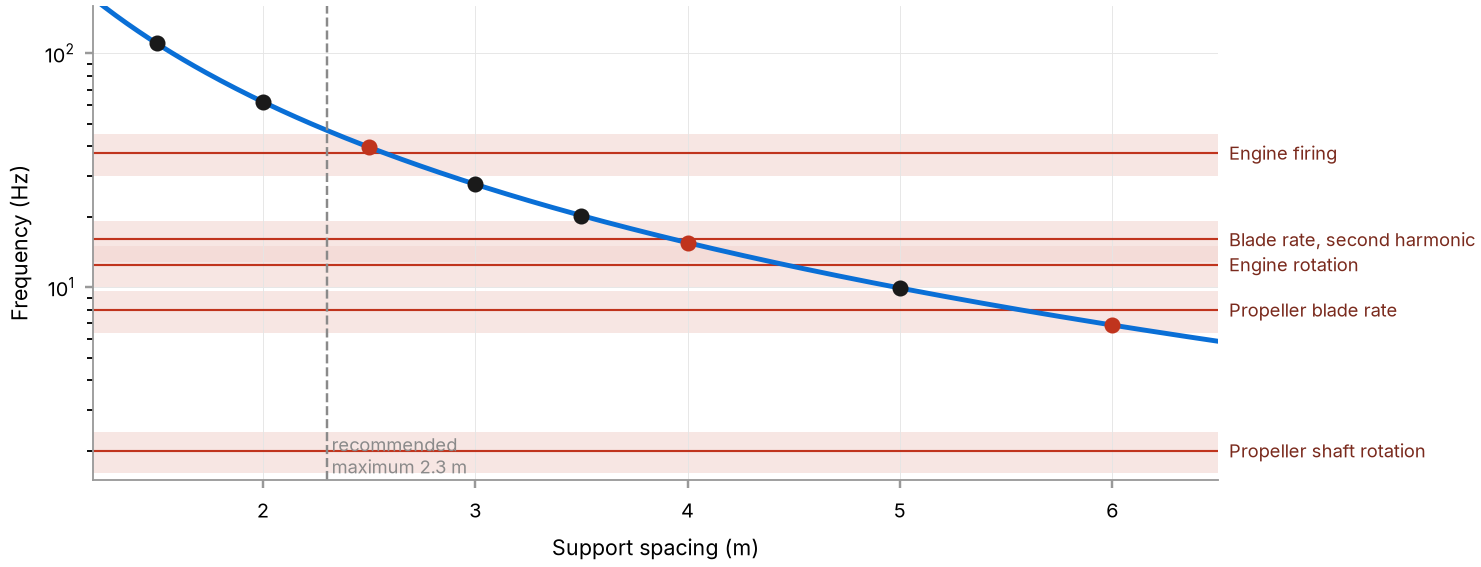
\includegraphics[width=\textwidth]{images/bracket-span-frequency.png}
\caption{Natural frequency of the NPS~4 span against support spacing, with
$\pm 20\%$ bands round each excitation. Red points fail the margin}
\label{fig:bracket-span}
\end{figure}

\begin{table}[H]
\centering
\caption{Pipe span against support spacing, NPS~4 seawater line}
\label{tab:span-sweep}
\small
\begin{tabular}{rrlrrl}
\toprule
\textbf{Spacing (m)} & \textbf{$f_n$ (Hz)} & \textbf{Nearest excitation} & \textbf{Margin} & \textbf{Stress (MPa)} & \textbf{Result}\\
\midrule
1.5 & 110.28 & Engine firing & 194.1\% & 2.2 & Passes\\
2.0 & 62.03 & Engine firing & 65.4\% & 3.9 & Passes\\
2.5 & 39.70 & Engine firing & 5.9\% & 6.1 & Fails\\
3.0 & 27.57 & Engine firing & 26.5\% & 8.8 & Passes\\
3.5 & 20.25 & Twice blade rate & 26.6\% & 12.0 & Passes\\
4.0 & 15.51 & Twice blade rate & 3.1\% & 15.7 & Fails\\
5.0 & 9.92 & Engine rotation & 20.6\% & 24.6 & Passes\\
6.0 & 6.89 & Blade rate & 13.8\% & 35.4 & Fails\\
\bottomrule
\end{tabular}
\end{table}

Figure~\ref{fig:bracket-size-sweep} repeats the case for pipe sizes NPS~2 to
NPS~12 at 3~m spacing. The recommended spacing rises from 1.7~m to 3.7~m,
because the stiffness of a pipe grows faster with diameter than its mass does.
It is set by frequency at every size. The bracket mass rises from 0.61~kg to
4.24~kg. The governing strength check moves from the bulkhead welds, at 9\% for
NPS~2, to the seat plate between the knees from NPS~10, at 82\%.

\begin{figure}[H]
\centering
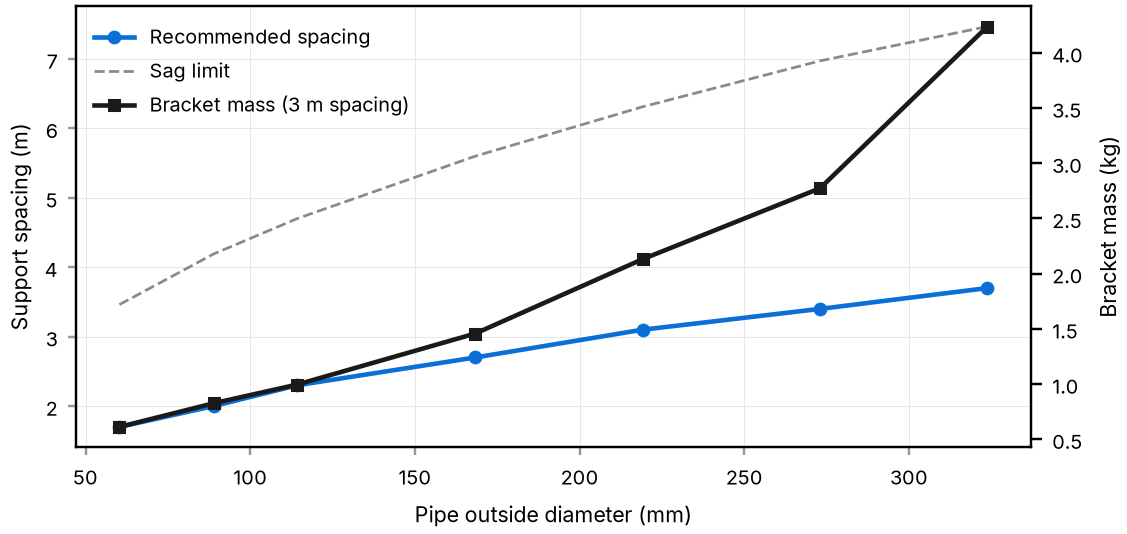
\includegraphics[width=0.8\textwidth]{images/bracket-size-sweep.png}
\caption{Recommended spacing and bracket mass against pipe size}
\label{fig:bracket-size-sweep}
\end{figure}

\subsection{Finite element results}

The peak von Mises stress away from the bulkhead face was 34.65~MPa, 7.7\%
below the hand value of 37.53~MPa for the seat plate between the knees
(Figure~\ref{fig:bracket-stress}). The hand model is a simply supported strip,
which ignores the restraint the knees give the seat edges, so it should be
higher. The peak changed by 0.54\% between the two finest meshes. The highest
stress anywhere in the model rose from 36.2~MPa to 47.6~MPa as the mesh was
refined. That value sits at the fixed edge against the bulkhead, where the
singularity described in Section~\ref{sec:fea} makes it meaningless, and the
assessed region excludes it for this reason. With a peak of 35~MPa against a
235~MPa yield, the factor of safety is 6.8.

\begin{figure}[H]
\centering
\begin{subfigure}{0.49\textwidth}
\centering
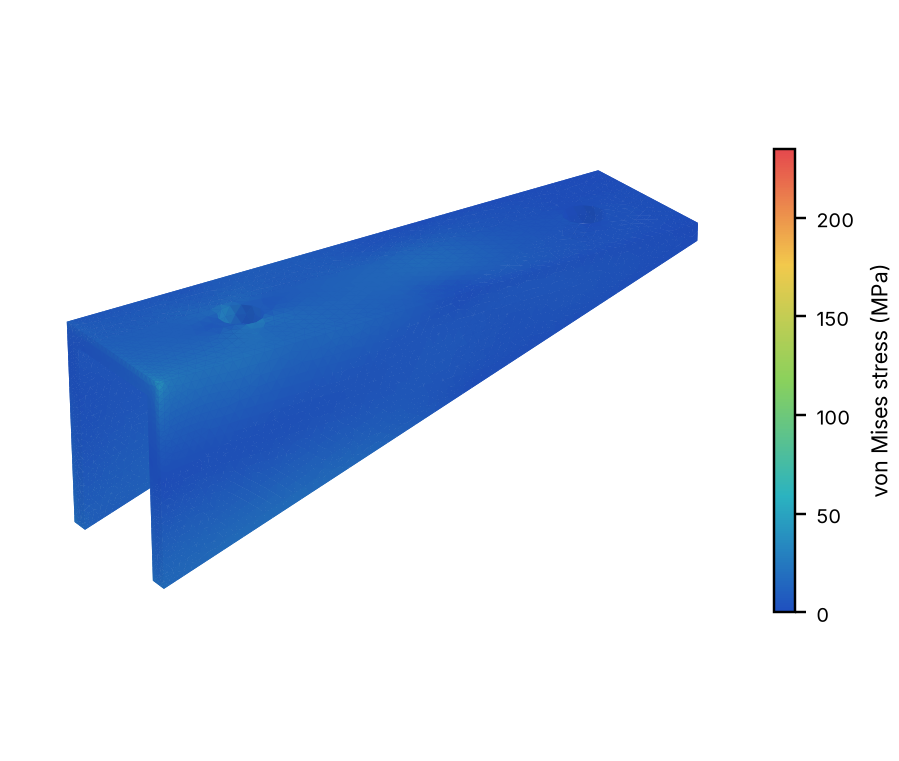
\includegraphics[width=\textwidth]{images/bracket-stress.png}
\caption{Von Mises stress}
\end{subfigure}
\hfill
\begin{subfigure}{0.49\textwidth}
\centering
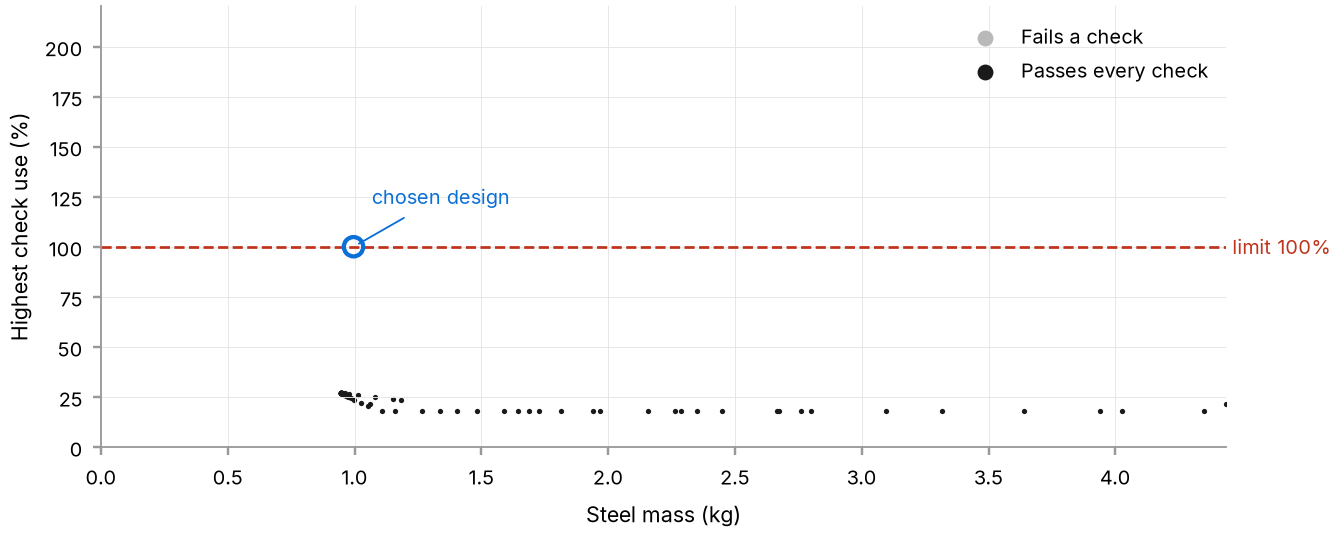
\includegraphics[width=\textwidth]{images/bracket-search.png}
\caption{Designs tried by the search}
\end{subfigure}
\caption{Bracket stress under the pipe load, and the search for the lightest
bracket}
\label{fig:bracket-stress}
\end{figure}

\section{Case study 3: patrol boat stabilizer fin}
\label{sec:fin-results}

\subsection{Loads}

At 18~knots, 9.26~m/s, the 1.4~m by 1.2~m fin has an area of 1.68~m$^2$ and
an effective aspect ratio of 2.33. Equation~\eqref{eq:whicker} gives a lift
slope of 2.708 per radian and, at 22$^\circ$, a lift coefficient of 1.090, of
which the non-linear term contributes 0.051. The foil model gives a lift of
80.49~kN. The UR S10 formula gives 66.74~kN, with $K_1 = 1.056$, $K_2 = 1.10$
and $K_3 = 0.8$. The foil model is 21\% higher and is used as the design force.
Because both methods scale with $V^2$, the ratio stays the same at every speed
(Figure~\ref{fig:fin-speed}).

The stock at 35\% chord lies 0.02$c$ aft of the 33\% centre of pressure, so the
rule minimum of $0.1Fc$ sets the twisting moment, $Q = 9.66$~kN\,m. The
bending moment is 56.34~kN\,m at the fin root and 72.44~kN\,m at the outer
bearing.

The UR S10 force formula is empirical and was written for rudders. A
stabilizer fin is a low-aspect-ratio foil, and at large angles it keeps
gaining lift through the cross-flow term of Equation~\eqref{eq:whicker}, past
the angle at which a two-dimensional section would stall
\cite{whicker1958,molland2007}. The result shows why the project derived the
load twice. Using the rule formula alone would have under-estimated the
design force by 17\% of the foil value.

\subsection{Pressure and cavitation}

The fin lift coefficient of 1.09 corresponds to a section angle of
8.5$^\circ$ on the two-dimensional NACA~0020 section. At that angle the panel
method gives the pressure distribution in Figure~\ref{fig:fin-pressure}. The
suction peak is close to the leading edge, at $C_{p,\text{min}} = -2.91$. At a
depth of 3~m and 18~knots the cavitation number is $\sigma = 2.953$, so the
advice check sits at 98.5\%. The fin is on the edge of leading-edge
cavitation at its largest angle.

\begin{figure}[H]
\centering
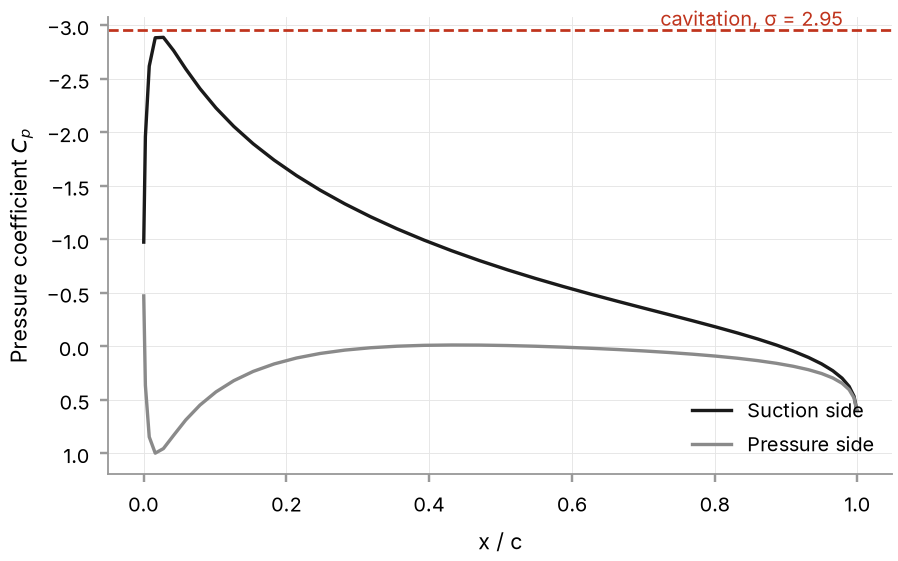
\includegraphics[width=0.65\textwidth]{images/fin-pressure.png}
\caption{Pressure on the NACA~0020 section at the angle that gives the fin's
lift coefficient, with the cavitation number at 18~knots}
\label{fig:fin-pressure}
\end{figure}

\subsection{Designs}

The search evaluated 3,780 combinations of skin, web and rib spacing over the
three targets, 1,260 per target. Table~\ref{tab:fin-designs} gives the three
designs. They differ only in the stock. The webs are at the 8~mm minimum of UR
S10, the skin is the thinnest plate in stock, 8~mm against a rule minimum of
7.54~mm, and five ribs at 350~mm pitch is the lightest arrangement in
every case, because the fin body runs at 38\% to 48\% of its strength.

\begin{table}[H]
\centering
\caption{Stabilizer fin designs at 18~knots}
\label{tab:fin-designs}
\small
\begin{tabularx}{\textwidth}{>{\raggedright\arraybackslash}Xrrr}
\toprule
& \textbf{Lightest} & \textbf{Balanced} & \textbf{Extra margin}\\
\midrule
Skin and webs (mm) & 8 & 8 & 8\\
Ribs, number at pitch (mm) & 5 at 350 & 5 at 350 & 5 at 350\\
Stock diameter (mm) & 160 & 170 & 180\\
Stock yield, EN 10083-3 (MPa) & 550 & 500 & 500\\
Mass of skin, spars and ribs (kg) & 315.4 & 315.4 & 315.4\\
Mass of stock (kg) & 142.1 & 160.4 & 179.8\\
Total mass (kg) & 457.5 & 475.8 & 495.2\\
Stock combined stress, UR S10.4.2 & 94.5\% & 78.8\% & 66.4\%\\
FEA stock stress near bearing (MPa) & 165.26 & 136.86 & 114.23\\
Beam theory at the same section (MPa) & 165.67 & 137.29 & 114.96\\
\bottomrule
\end{tabularx}
\end{table}

Table~\ref{tab:fin-checks-result} lists the checks on the lightest fin. The
stock in combined bending and twist at the outer bearing governs at 94.5\%.
The fit checks on plate thickness are close to their limits, the skin at
94.3\% of the plating formula and the webs exactly at the 8~mm minimum. The
fin body is lightly stressed, and the tip deflects 0.89~mm.

\begin{table}[H]
\centering
\caption{Checks on the lightest fin}
\label{tab:fin-checks-result}
\small
\begin{tabularx}{\textwidth}{>{\raggedright\arraybackslash}Xrrlr}
\toprule
\textbf{Check} & \textbf{Demand} & \textbf{Capacity} & \textbf{Unit} & \textbf{Use}\\
\midrule
Stock twisting, S10.4.1 & 12.0 & 110.7 & MPa & 10.9\%\\
Stock bending and twisting at the outer bearing, S10.4.2 & 181.6 & 192.1 & MPa & 94.5\%\\
Stock fits inside the foil & 160 & 214.1 & mm & 74.7\%\\
Fin body bending at the root, S10.5.1 & 55.7 & 146.1 & MPa & 38.1\%\\
Spar web shear at the root, S10.5.1 & 31.2 & 66.4 & MPa & 47.0\%\\
Fin skin combined stress, S10.5.1 & 56.3 & 159.4 & MPa & 35.3\%\\
Skin plate thickness, S10.5.2 & 7.54 & 8 & mm & 94.3\%\\
Spar and rib web thickness, S10.5.2 & 8 & 8 & mm & 100.0\%\\
Skin panel buckling & 55.7 & 116.5 & MPa & 47.8\%\\
Fin tip deflection & 0.89 & 10 & mm & 8.9\%\\
Cavitation at the largest fin angle (advice) & 2.91 & 2.953 & ratio & 98.5\%\\
\bottomrule
\end{tabularx}
\end{table}

The rule capacities for the stock do not change between the designs, though
the stock yield falls from 550~MPa to 500~MPa above 160~mm diameter. UR S10
caps the yield used in the material factor at $\min(0.7\sigma_T, 450)$~MPa.
With a tensile strength of 750~MPa that cap is 450~MPa, below both yields, so
$k = 0.614$ in every case and the combined limit is $118/k = 192.1$~MPa.

\subsection{Finite element results}

The stock model of the lightest design gave 165.26~MPa in the assessed region,
0.25\% below beam theory at the same section (Figure~\ref{fig:fin-stock}). The
peak changed by 0.12\% between the two finest meshes. The highest stress in
the whole model, 190.2~MPa, is at the fixed bearing face and is excluded for
the reason given in Section~\ref{sec:fea}. Against the 550~MPa yield, the
factor of safety is 3.33. The UR S10 check is far more severe than this, at
94.5\%, because its limit of 192.1~MPa is about 35\% of yield. The rule
limit, not the elastic stress, decides the stock size.

\begin{figure}[H]
\centering
\begin{subfigure}{0.49\textwidth}
\centering
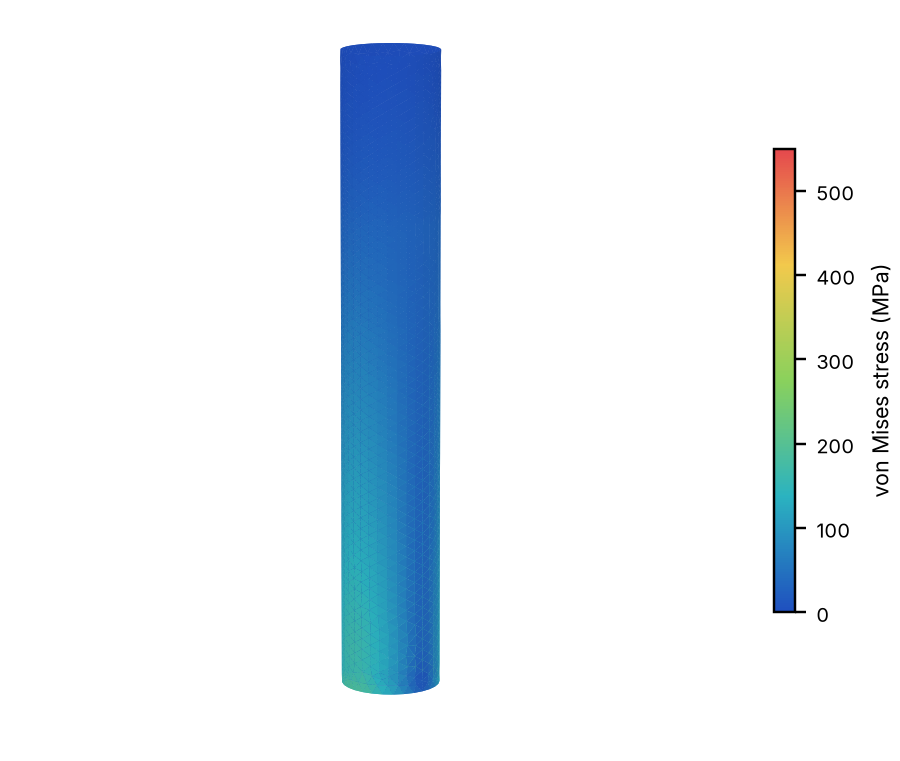
\includegraphics[width=\textwidth]{images/fin-stock-stress.png}
\caption{Von Mises stress in the stock}
\end{subfigure}
\hfill
\begin{subfigure}{0.49\textwidth}
\centering
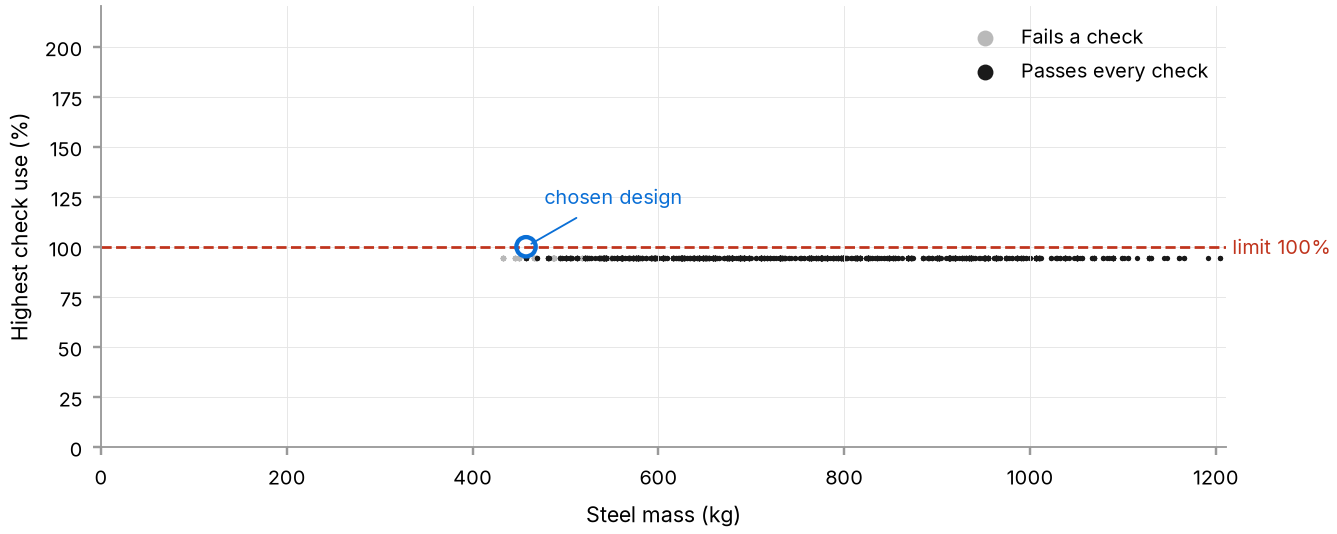
\includegraphics[width=\textwidth]{images/fin-search.png}
\caption{Designs tried by the search}
\end{subfigure}
\caption{Stock stress under the fin force and twist, and the search for the
lightest fin}
\label{fig:fin-stock}
\end{figure}

Figure~\ref{fig:convergence} brings together the mesh studies of the three
case studies. In each case the assessed peak settles on the first refinement,
and for the bracket and the fin it lies close to the hand value.

\begin{figure}[H]
\centering
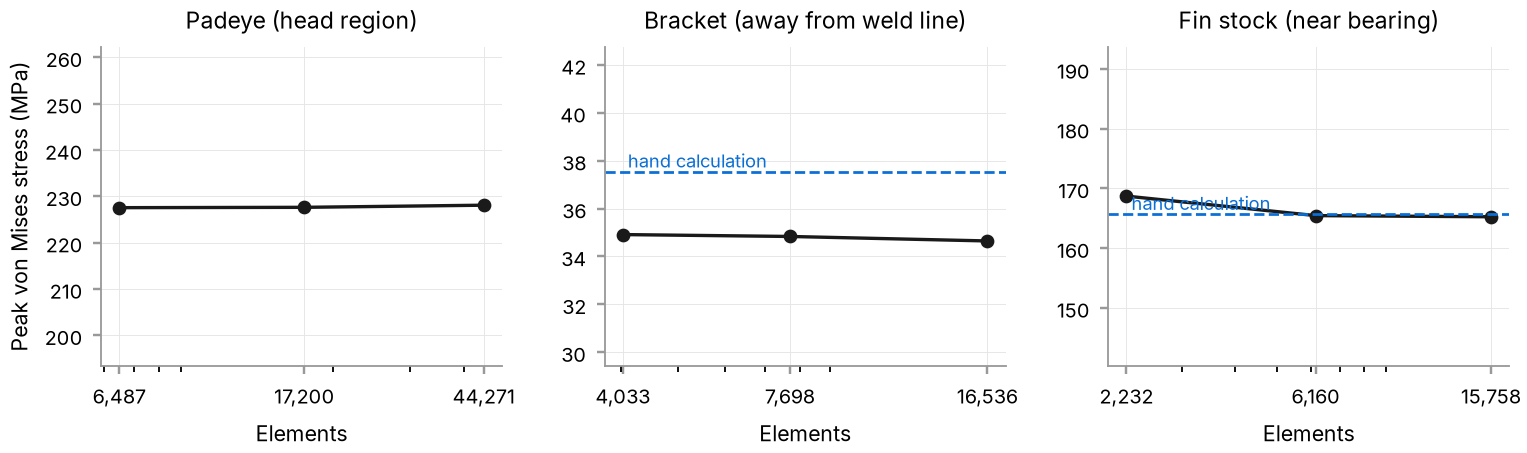
\includegraphics[width=\textwidth]{images/convergence.png}
\caption{Assessed peak stress against the number of elements for the three
lightest designs, with the hand values where they apply}
\label{fig:convergence}
\end{figure}

\subsection{Response to ship speed}

Figure~\ref{fig:fin-speed} and Figure~\ref{fig:fin-stock-sweep} show the fin
sized for speeds from 10~knots to 24~knots. The design force rises from
24.8~kN to 143.1~kN and the stock from 110~mm to 195~mm. The fin mass rises
from 370~kg to 539~kg, and nearly all of that increase is in the stock,
because the skin and webs stay at the 8~mm minimum. The cavitation number falls
with the square of speed, while $-C_{p,\text{min}}$ stays at 2.91 because the
angle is fixed. Cavitation begins between 18 and 20~knots. At 20~knots
$\sigma = 2.39$, well below 2.91. For this fin, cavitation would limit the
largest angle at high speed before the structure does.

\begin{figure}[H]
\centering
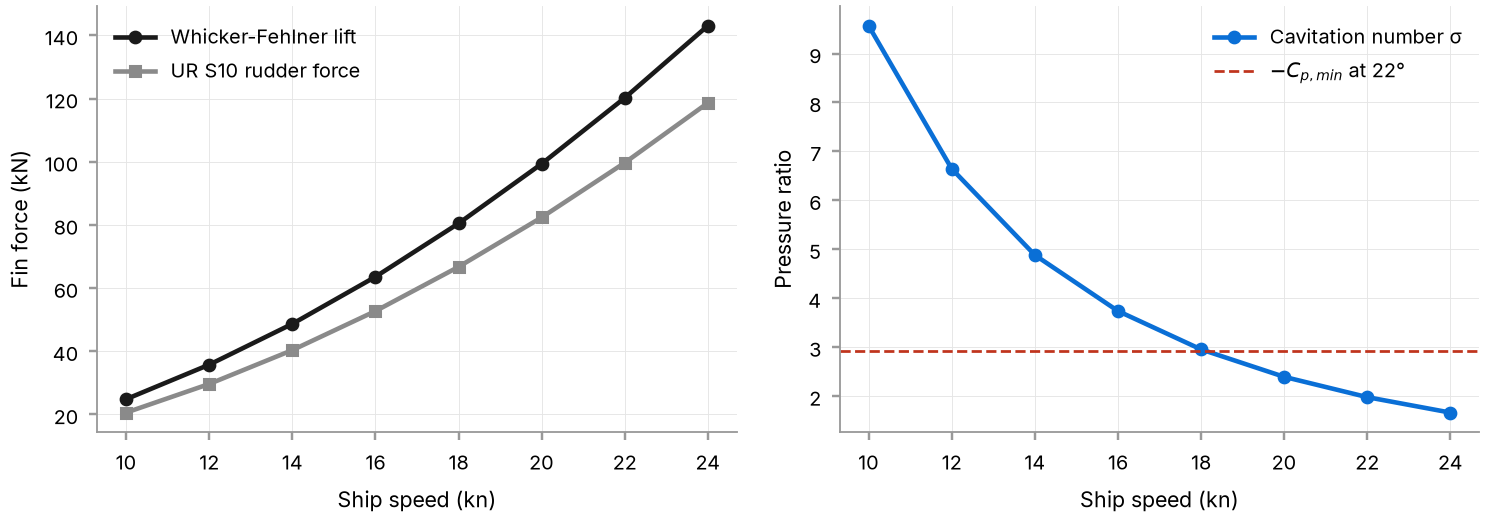
\includegraphics[width=\textwidth]{images/fin-speed-sweep.png}
\caption{Fin force from the two load methods, and cavitation number against
the lowest pressure, over ship speed}
\label{fig:fin-speed}
\end{figure}

\begin{figure}[H]
\centering
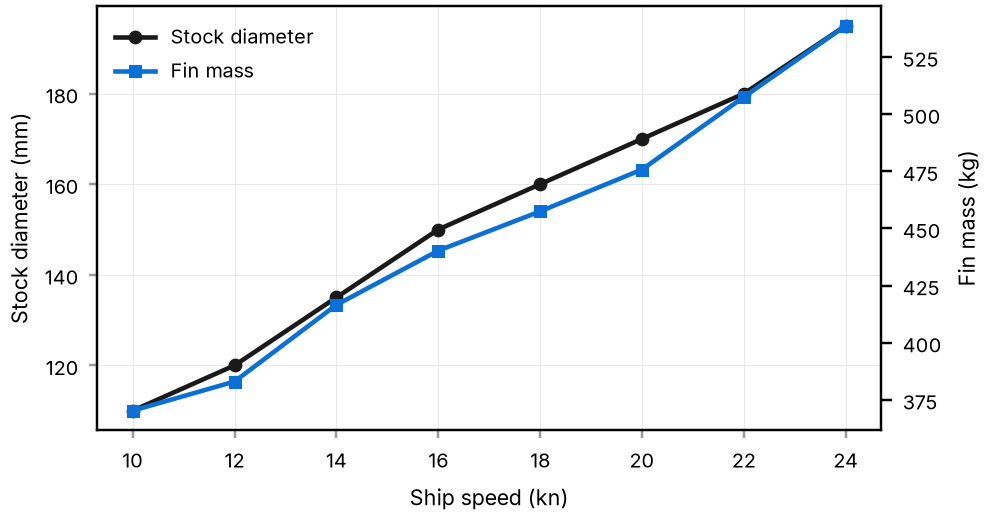
\includegraphics[width=0.7\textwidth]{images/fin-stock-sweep.png}
\caption{Stock diameter and fin mass against ship speed}
\label{fig:fin-stock-sweep}
\end{figure}

\section{Calculation package and application}
\label{sec:results-package}

Each design produced a PDF calculation package of 0.34~MB to 0.64~MB.
Figure~\ref{fig:padeye-report} shows three pages from the package of the
lightest padeye. The summary page gives the design, the loads and the
governing check. The drawing is dimensioned from the same design record as the
STEP file. The check pages show each formula with its values, its result and
its source, so that a checker can follow the calculation without the
software.

\begin{figure}[H]
\centering
\begin{subfigure}{0.32\textwidth}
\centering
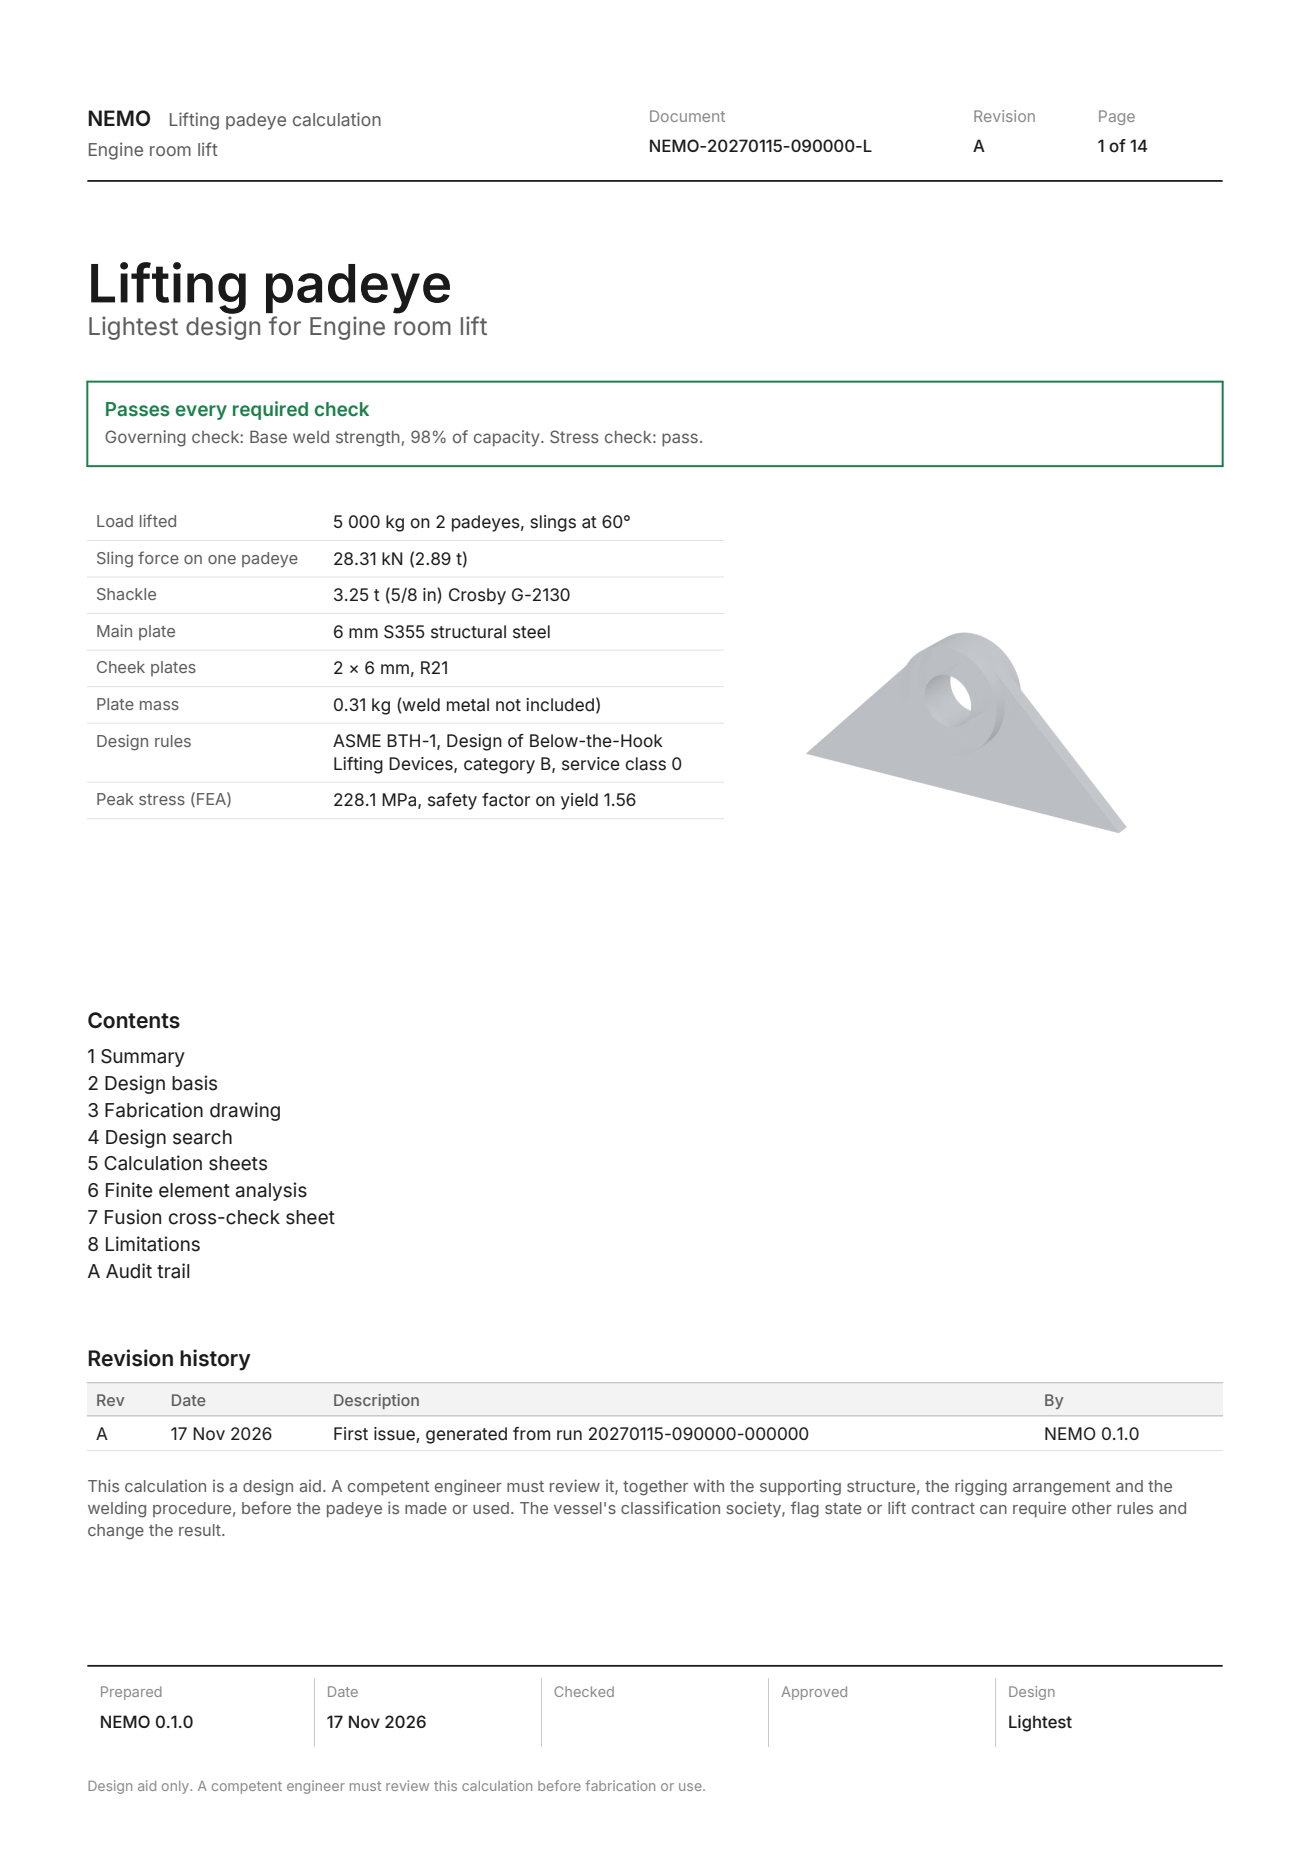
\includegraphics[width=\textwidth]{images/padeye-report-summary.png}
\caption{Summary}
\end{subfigure}
\hfill
\begin{subfigure}{0.32\textwidth}
\centering
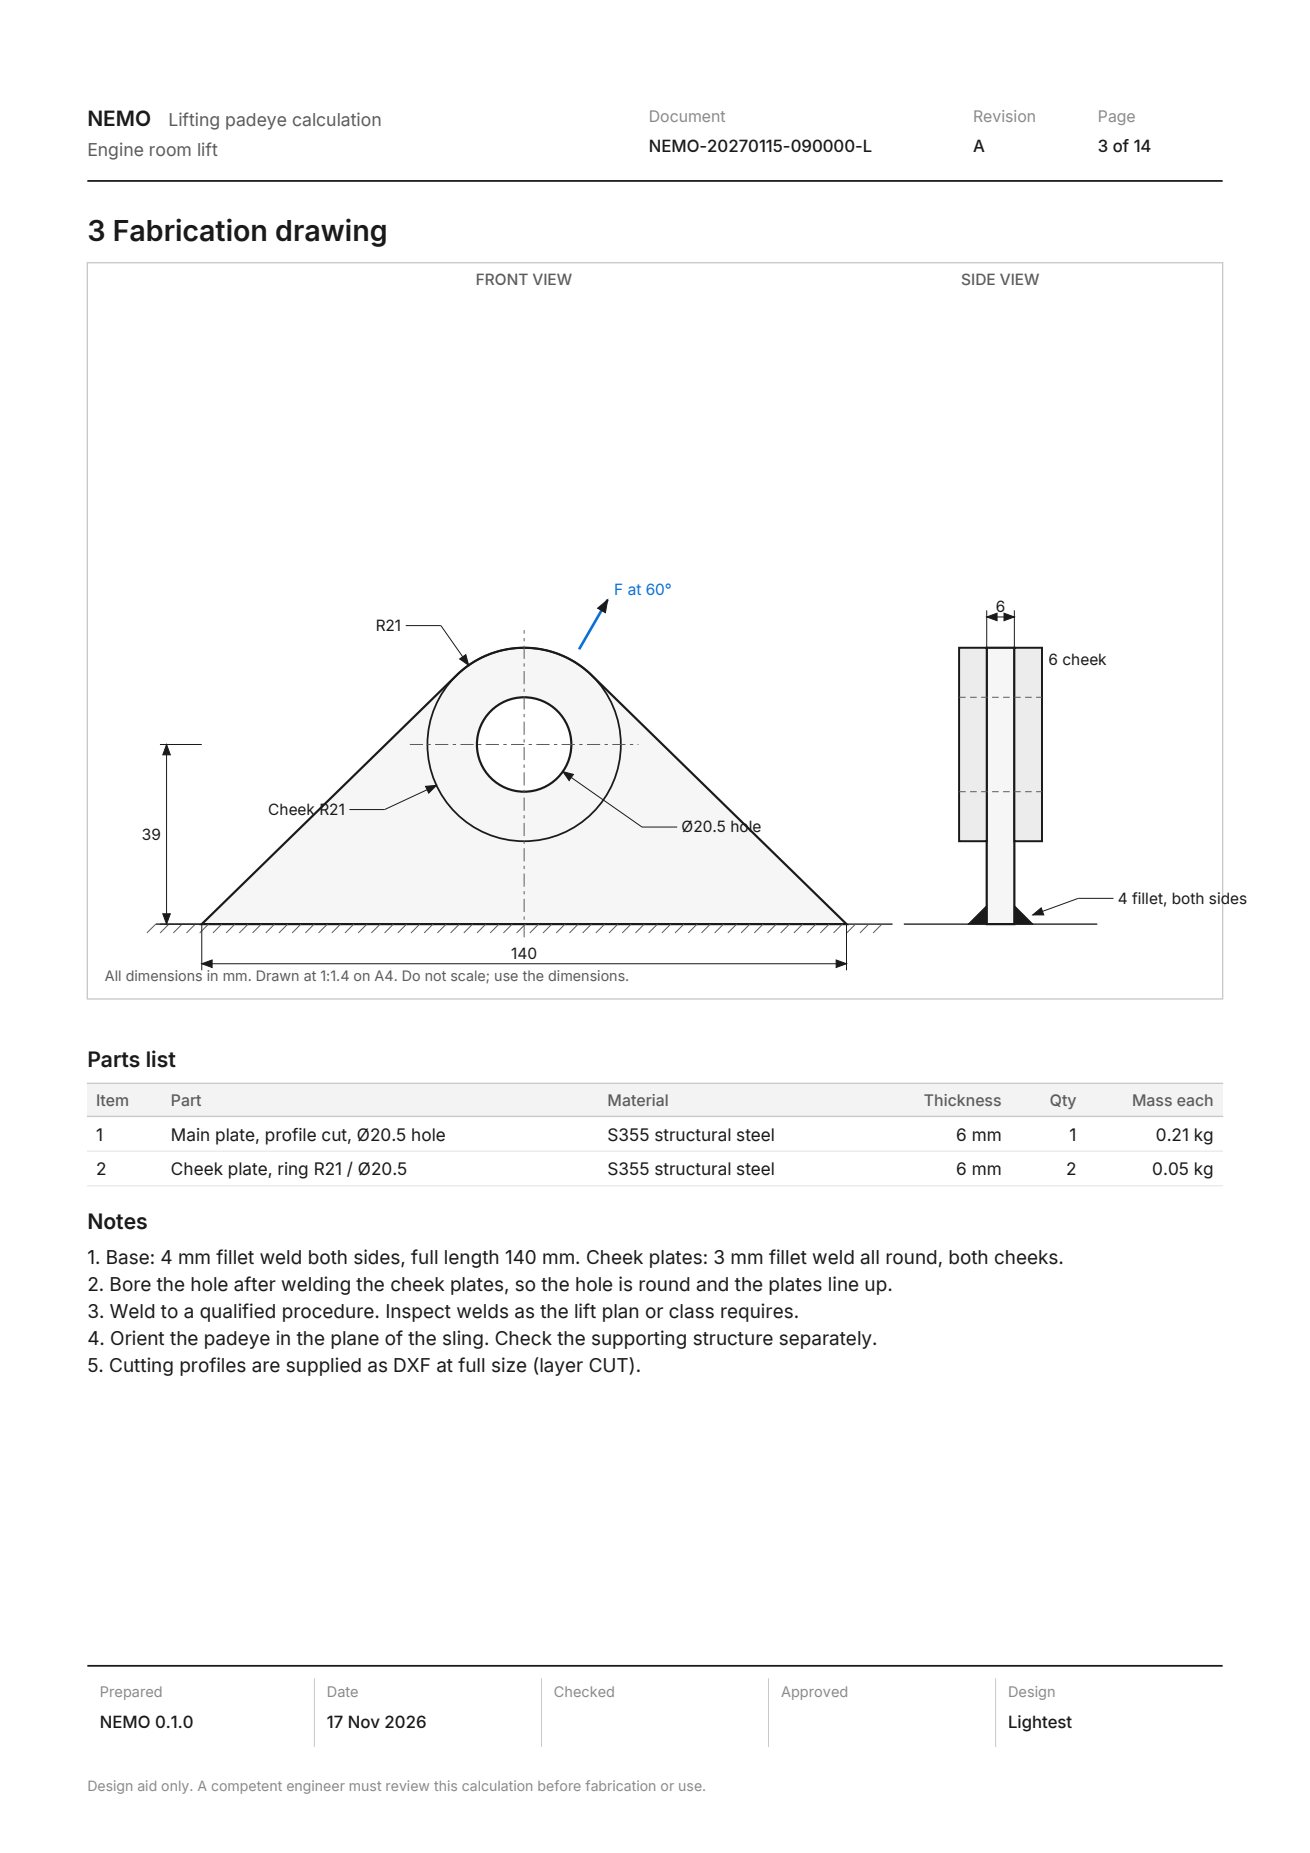
\includegraphics[width=\textwidth]{images/padeye-report-drawing.png}
\caption{Drawing}
\end{subfigure}
\hfill
\begin{subfigure}{0.32\textwidth}
\centering
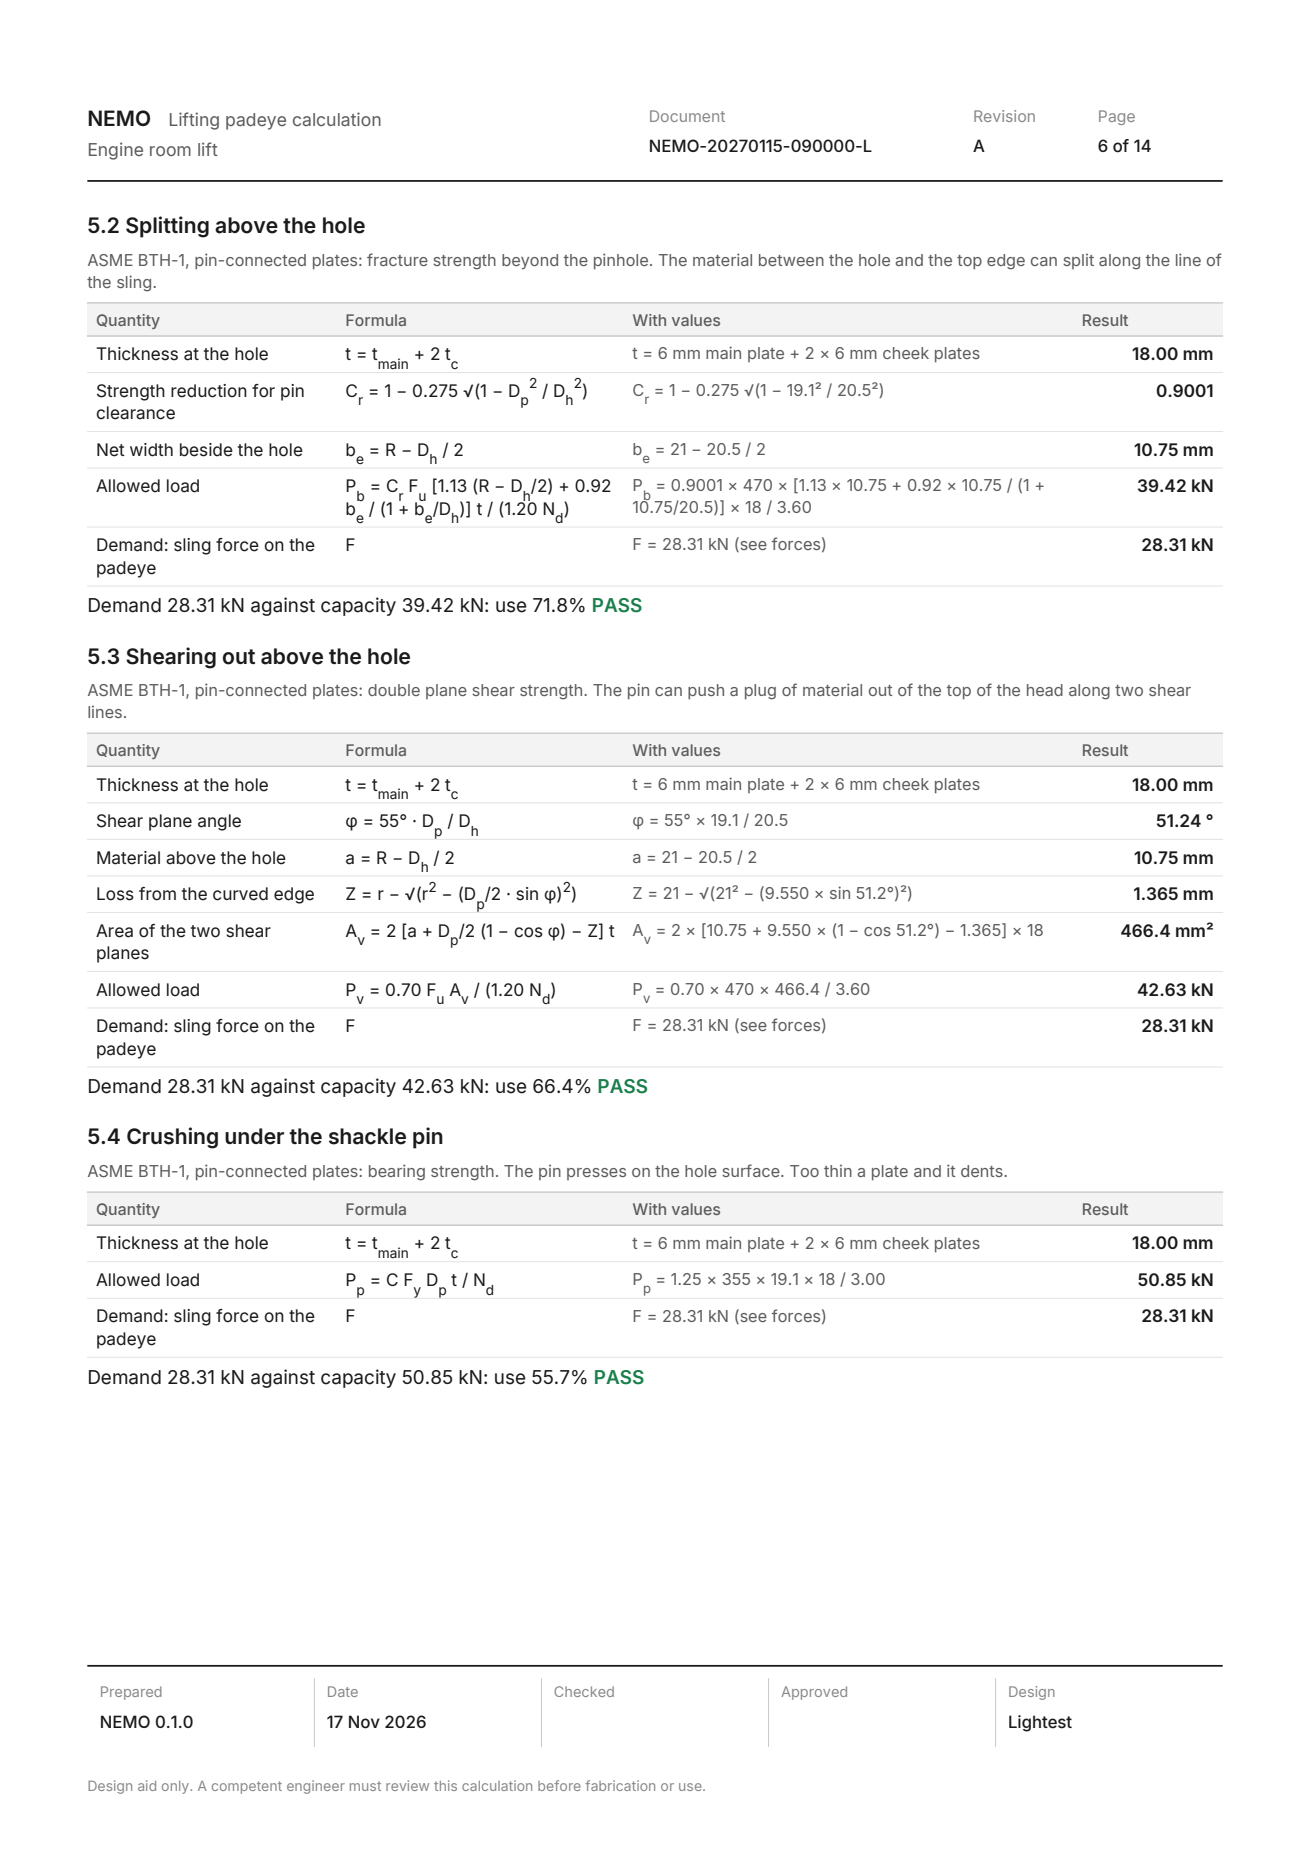
\includegraphics[width=\textwidth]{images/padeye-report-calc.png}
\caption{Check working}
\end{subfigure}
\caption{Pages from the calculation package of the lightest padeye}
\label{fig:padeye-report}
\end{figure}

\begin{figure}[H]
\centering
\begin{subfigure}{0.24\textwidth}
\centering
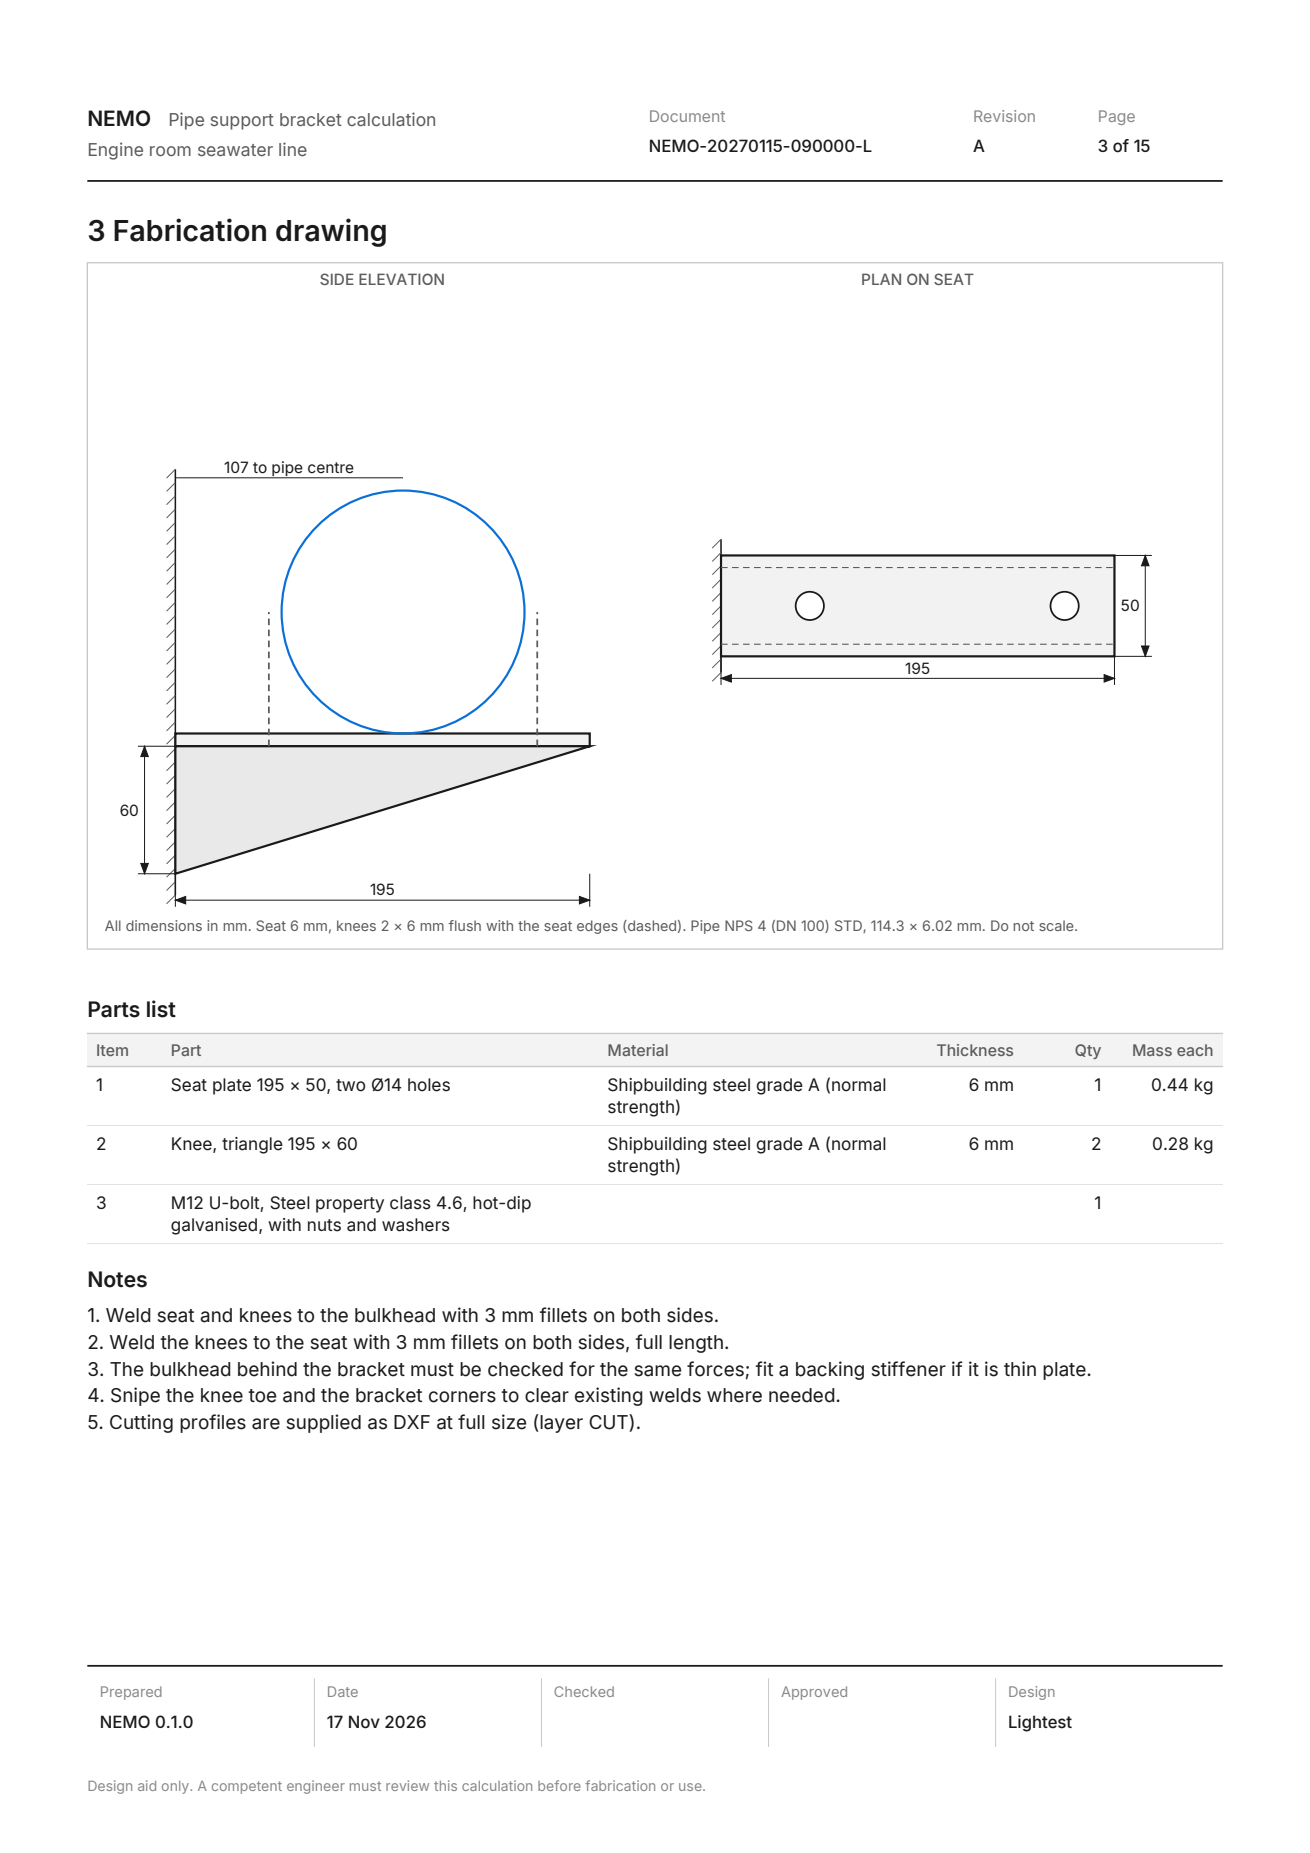
\includegraphics[width=\textwidth]{images/bracket-report-drawing.png}
\caption{Bracket drawing}
\end{subfigure}
\hfill
\begin{subfigure}{0.24\textwidth}
\centering
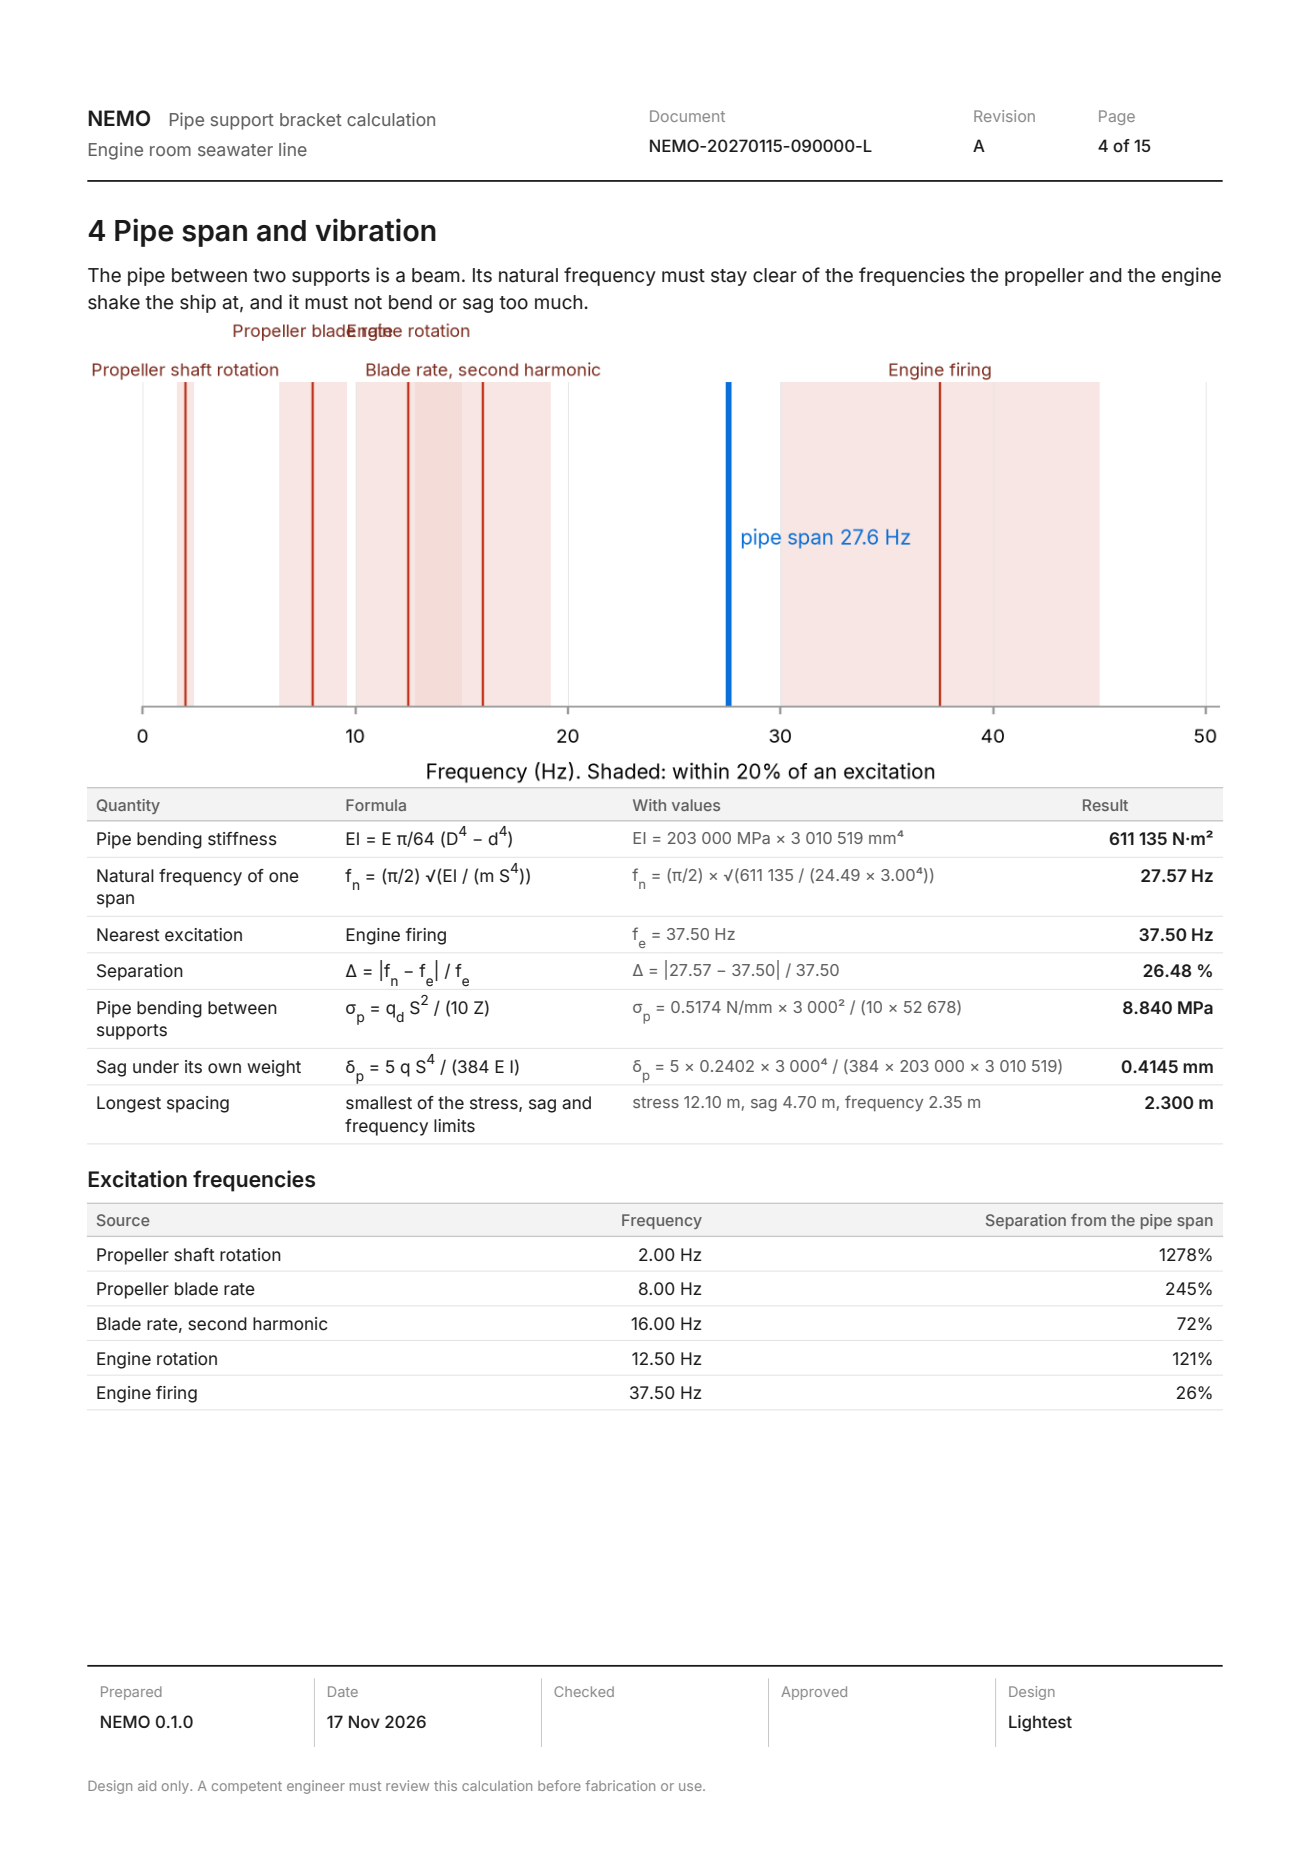
\includegraphics[width=\textwidth]{images/bracket-report-span.png}
\caption{Pipe span}
\end{subfigure}
\hfill
\begin{subfigure}{0.24\textwidth}
\centering
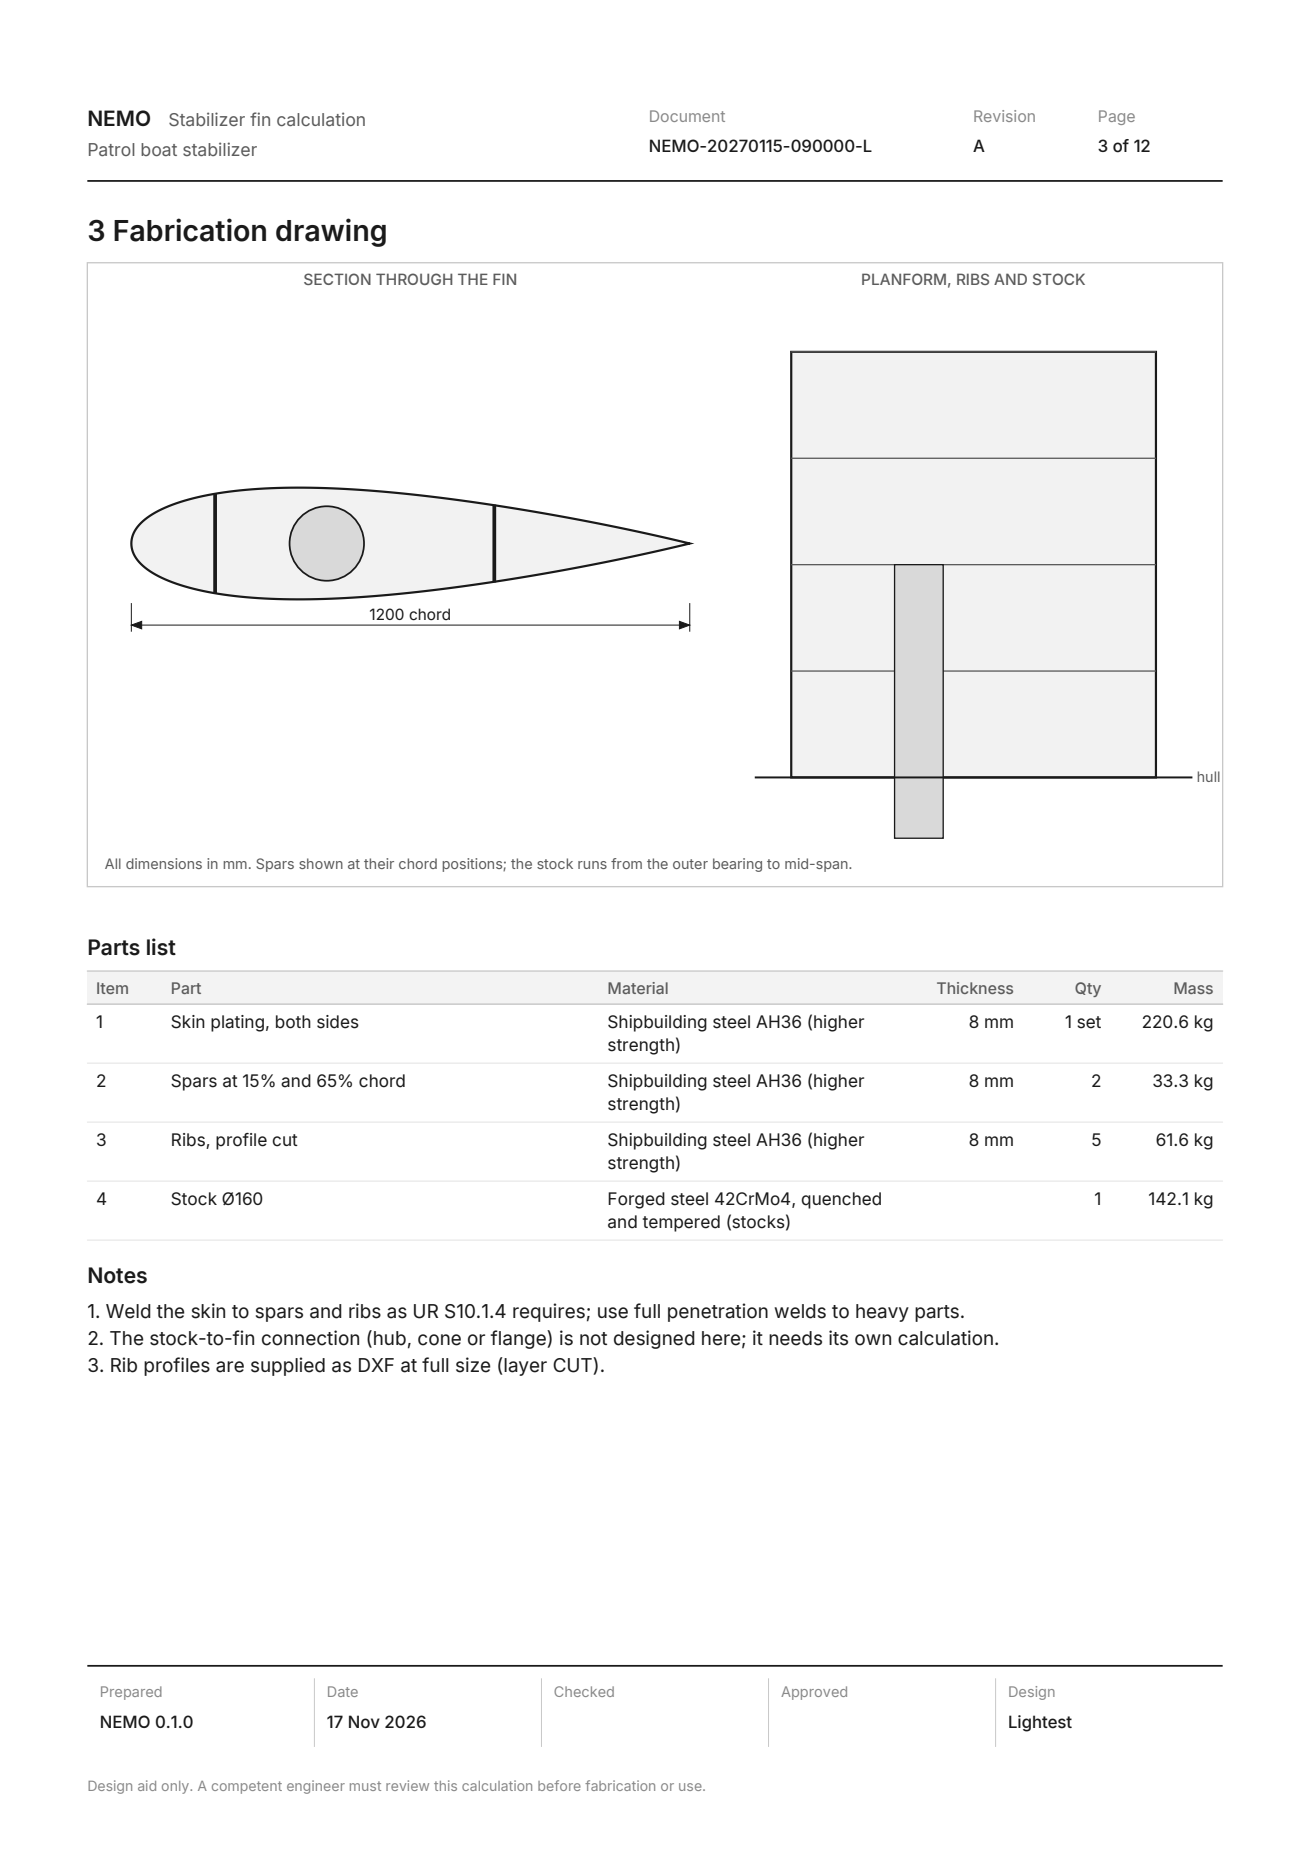
\includegraphics[width=\textwidth]{images/fin-report-drawing.png}
\caption{Fin drawing}
\end{subfigure}
\hfill
\begin{subfigure}{0.24\textwidth}
\centering
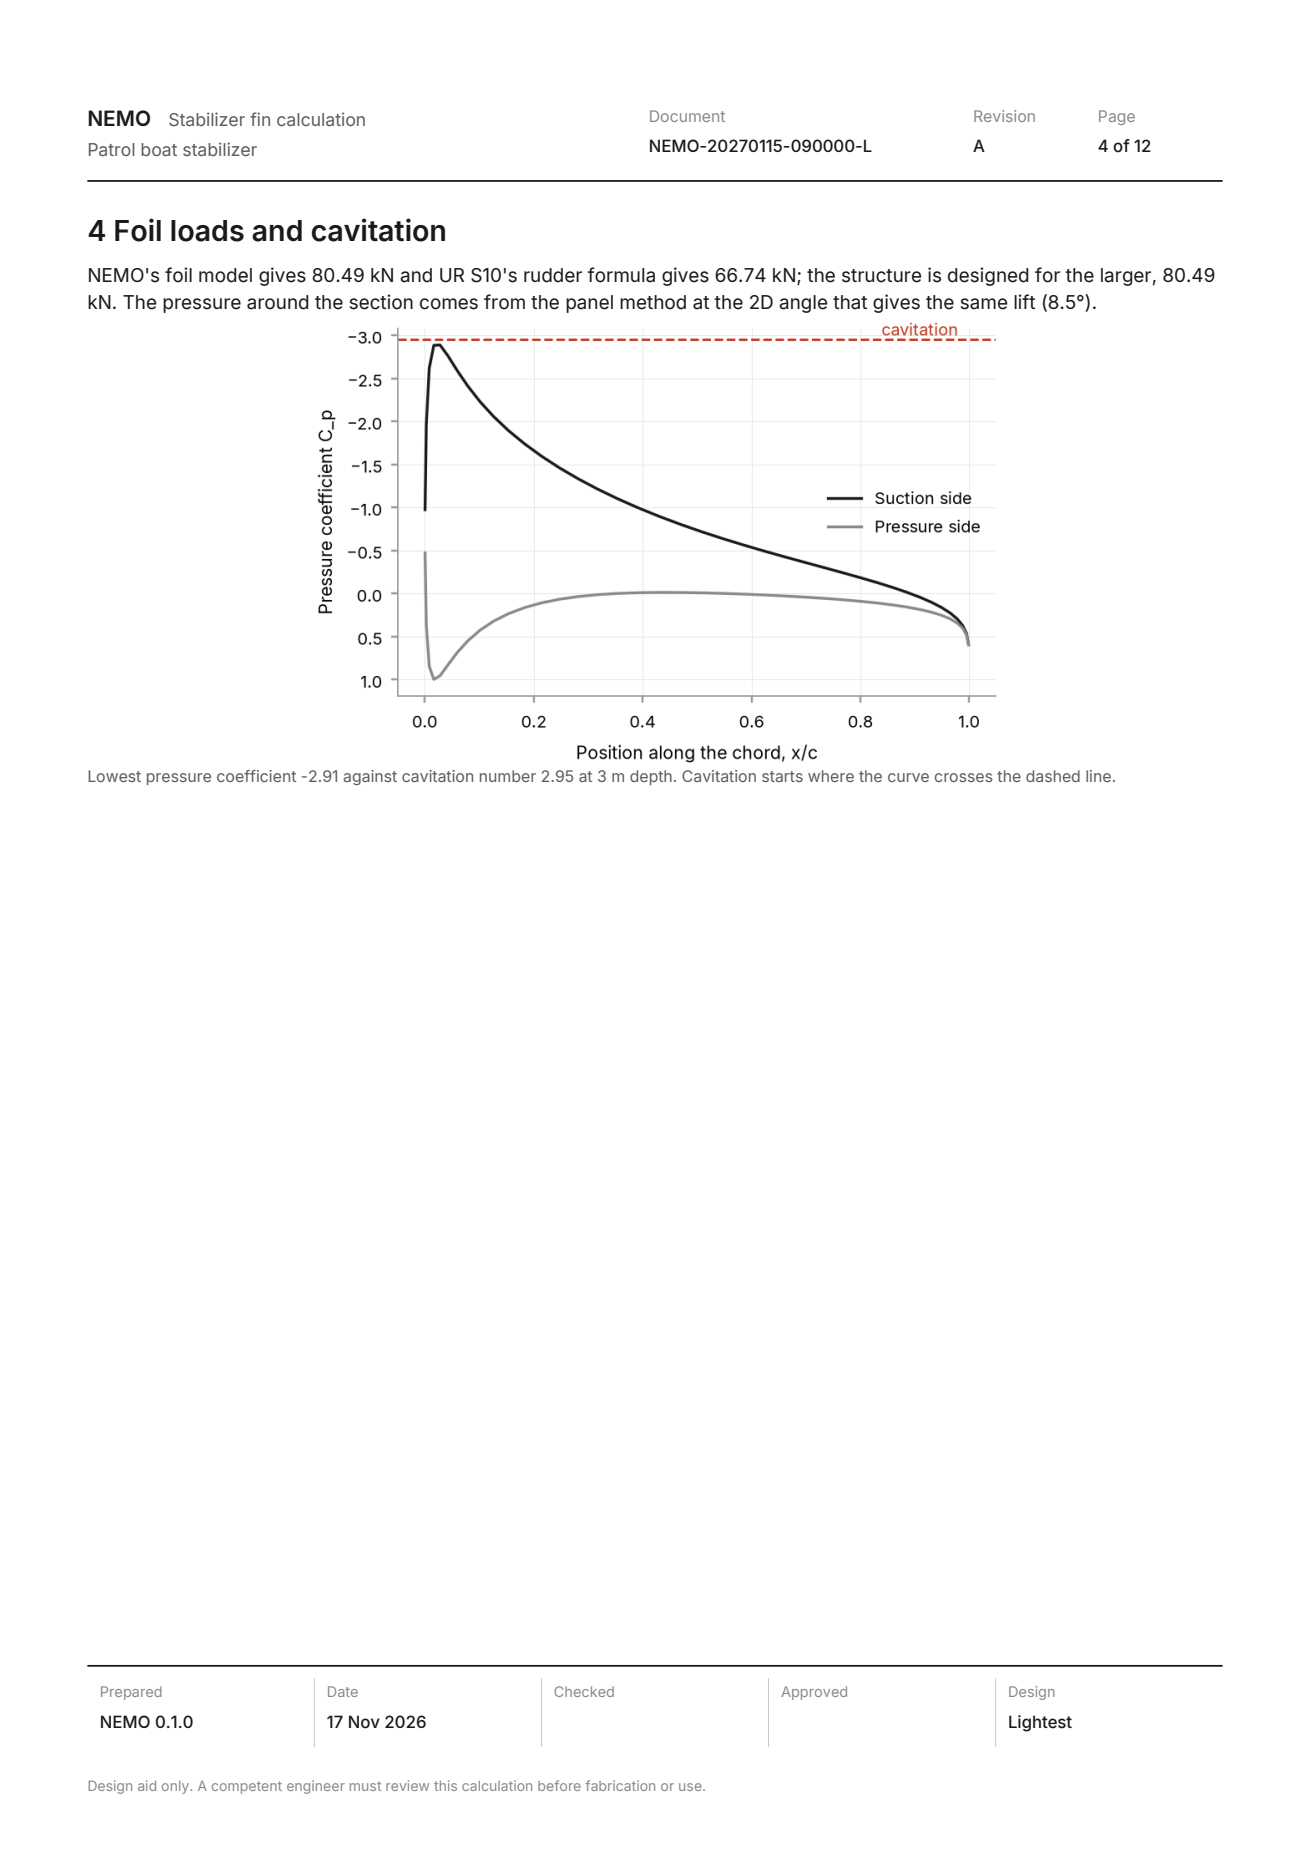
\includegraphics[width=\textwidth]{images/fin-report-foil.png}
\caption{Foil loads}
\end{subfigure}
\caption{Pages from the bracket and fin calculation packages}
\label{fig:other-reports}
\end{figure}

Figures~\ref{fig:app-results} to~\ref{fig:app-record} show the results
screens. The padeye results show the three designs side by side, the
dimensions of the selected one and its 3D model with the shackle and sling in
place. Selecting a check opens its working. The fin results show the stress in
the stock on the 3D model. The engineering record of the bracket lists the
steps of the run with their numbers, drawn from the engineering log.

\begin{figure}[H]
\centering
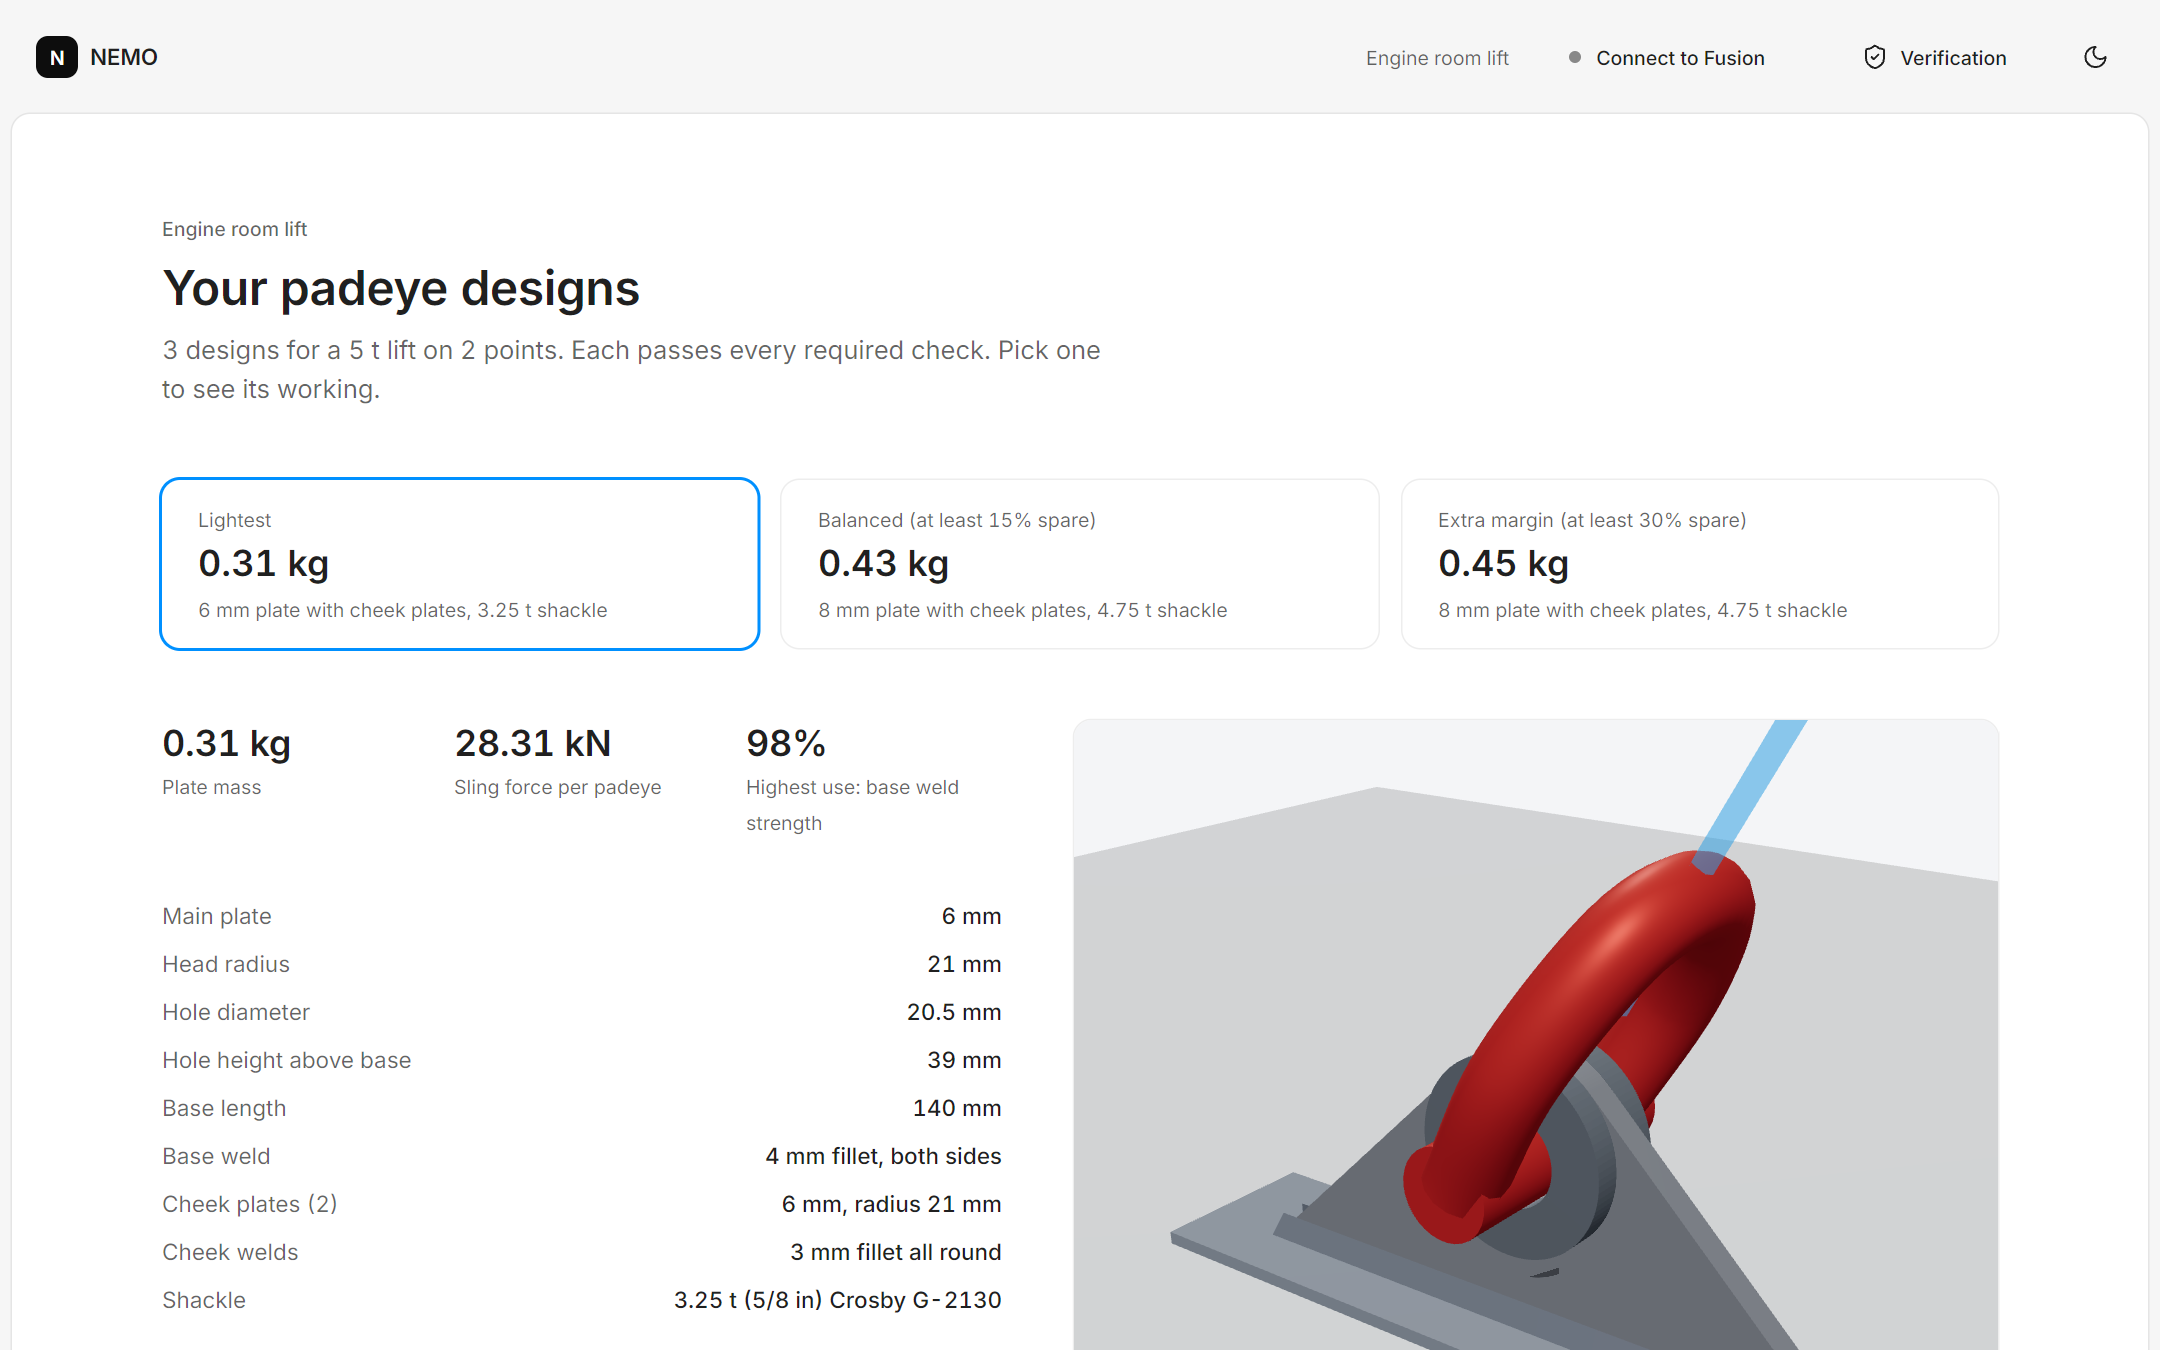
\includegraphics[width=0.85\textwidth]{images/app-padeye-results.png}
\caption{Padeye results, with the lightest of the three designs selected}
\label{fig:app-results}
\end{figure}

\begin{figure}[H]
\centering
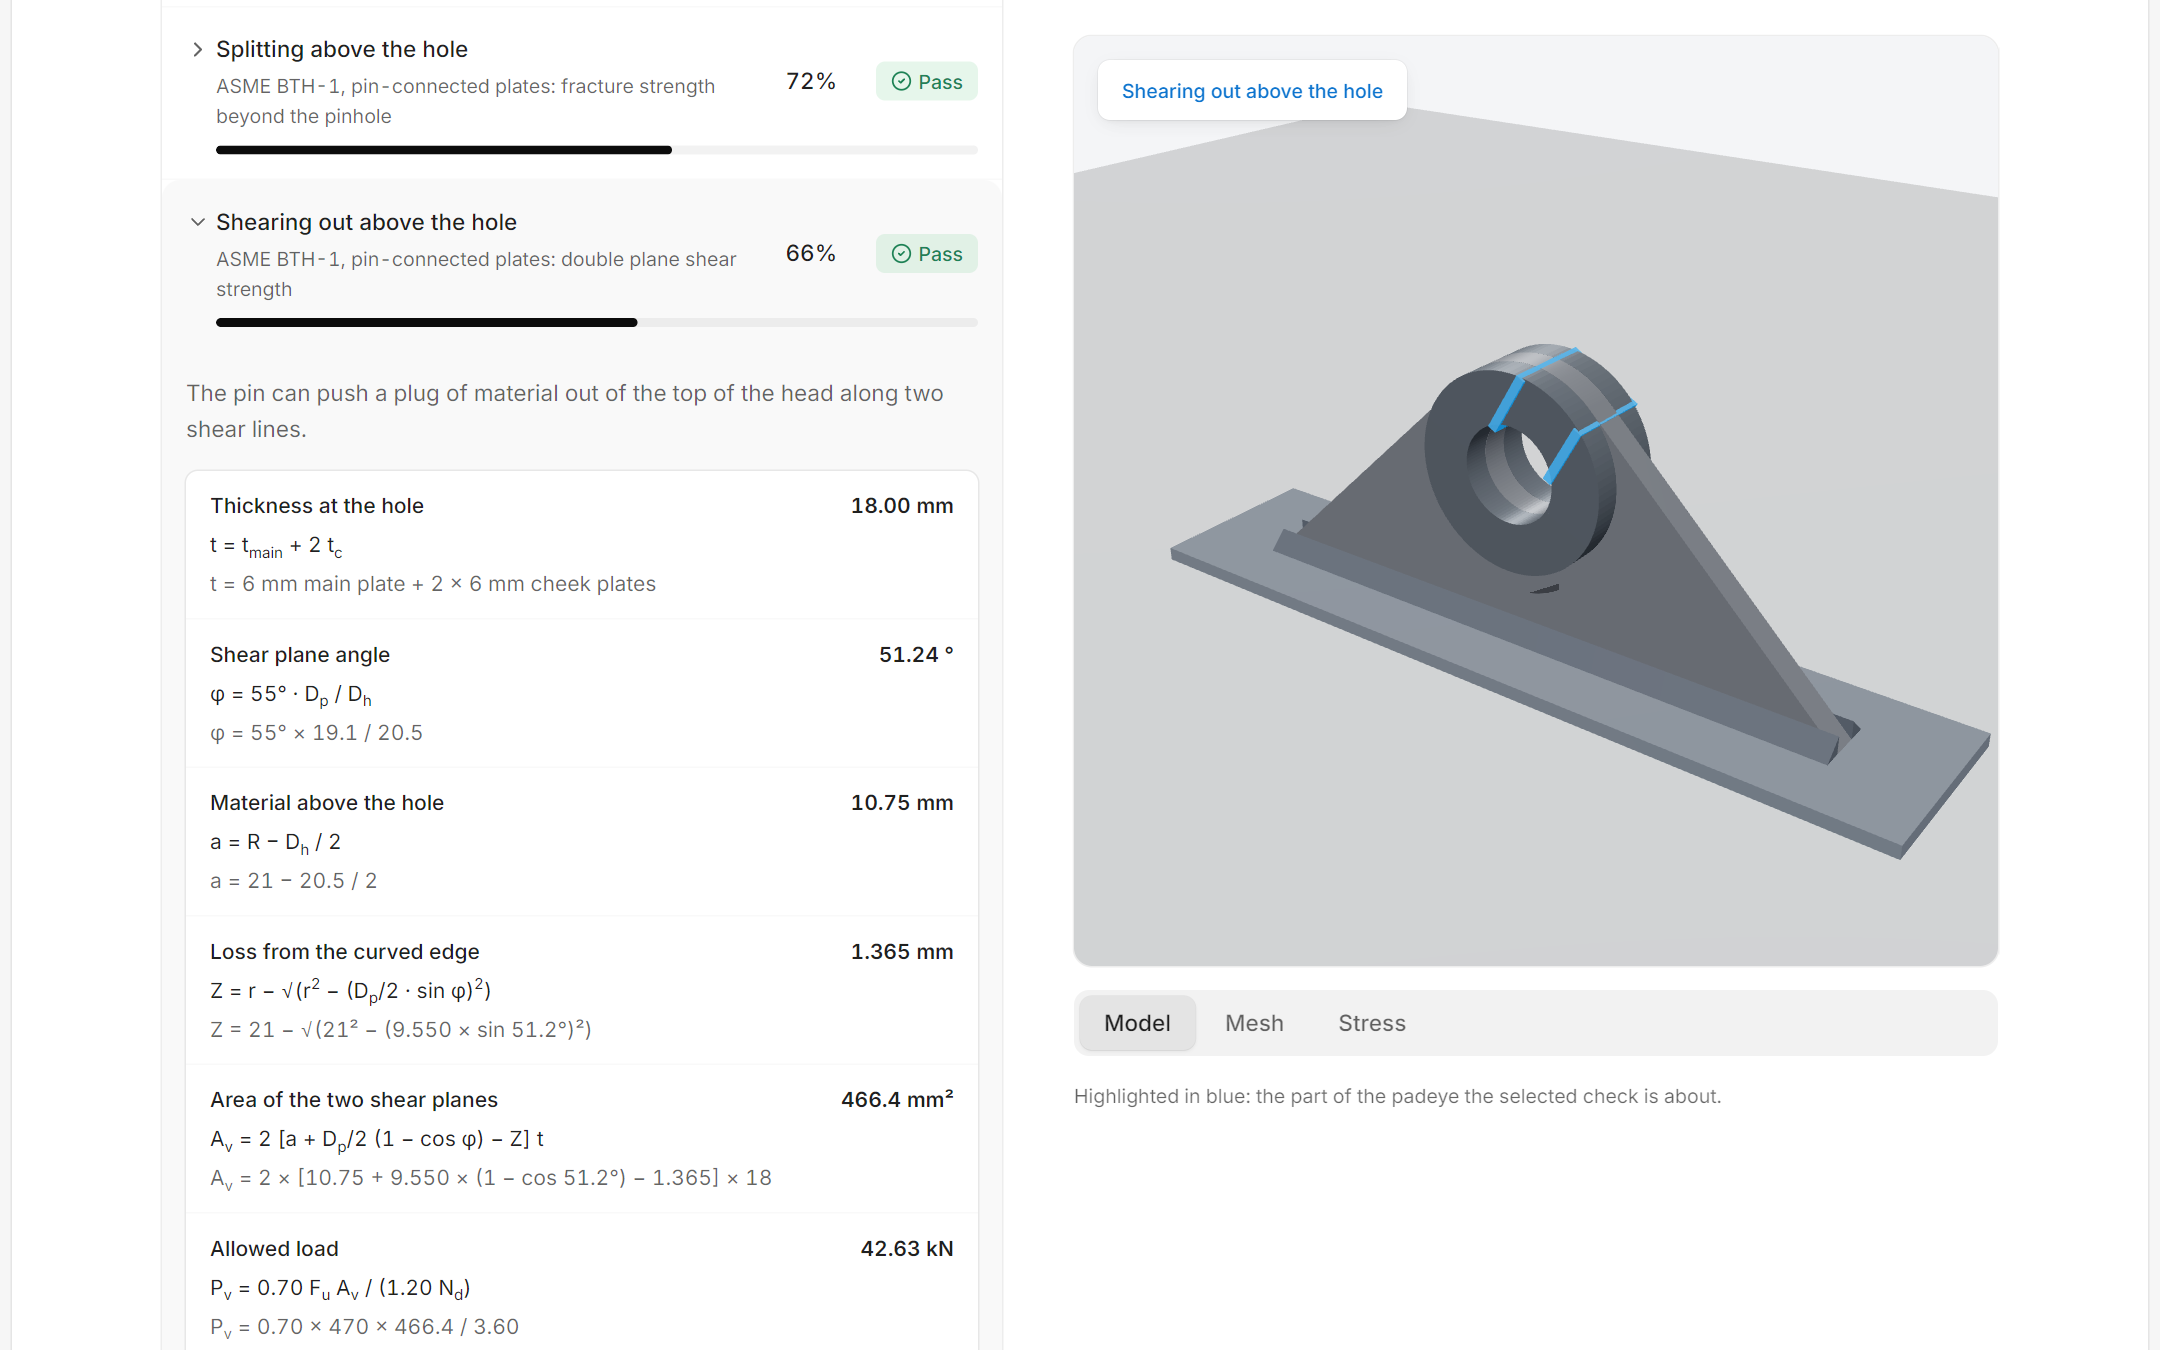
\includegraphics[width=0.85\textwidth]{images/app-padeye-check-working.png}
\caption{Working of a padeye check, as shown in the application}
\label{fig:app-check-working}
\end{figure}

\begin{figure}[H]
\centering
\begin{subfigure}{0.49\textwidth}
\centering
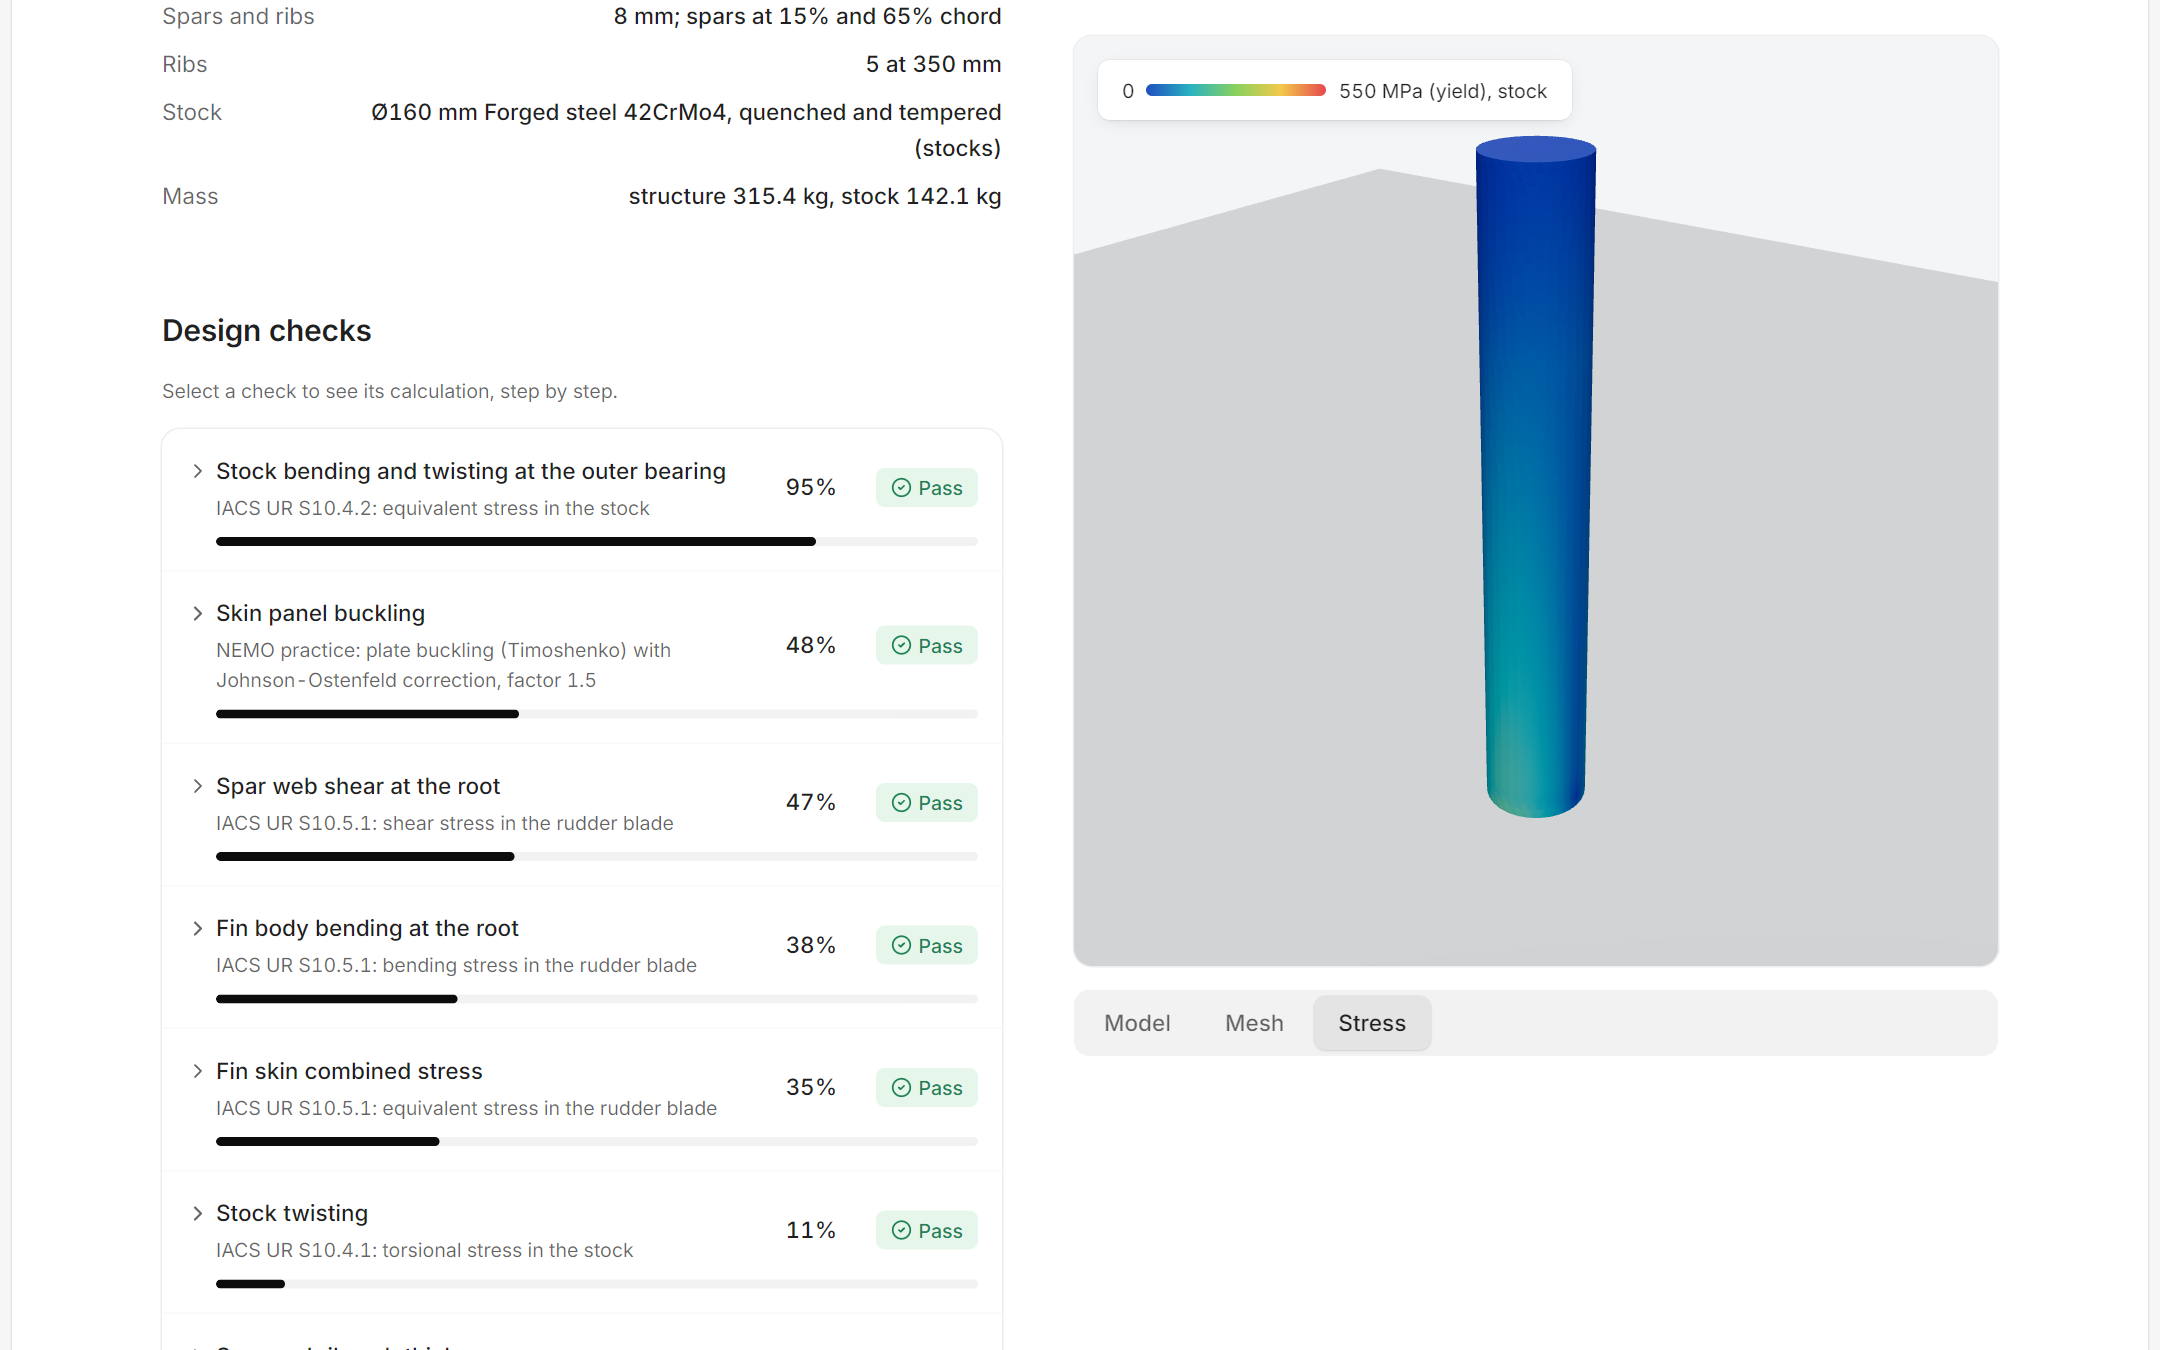
\includegraphics[width=\textwidth]{images/app-fin-results-stress.png}
\caption{Fin stock stress}
\end{subfigure}
\hfill
\begin{subfigure}{0.49\textwidth}
\centering
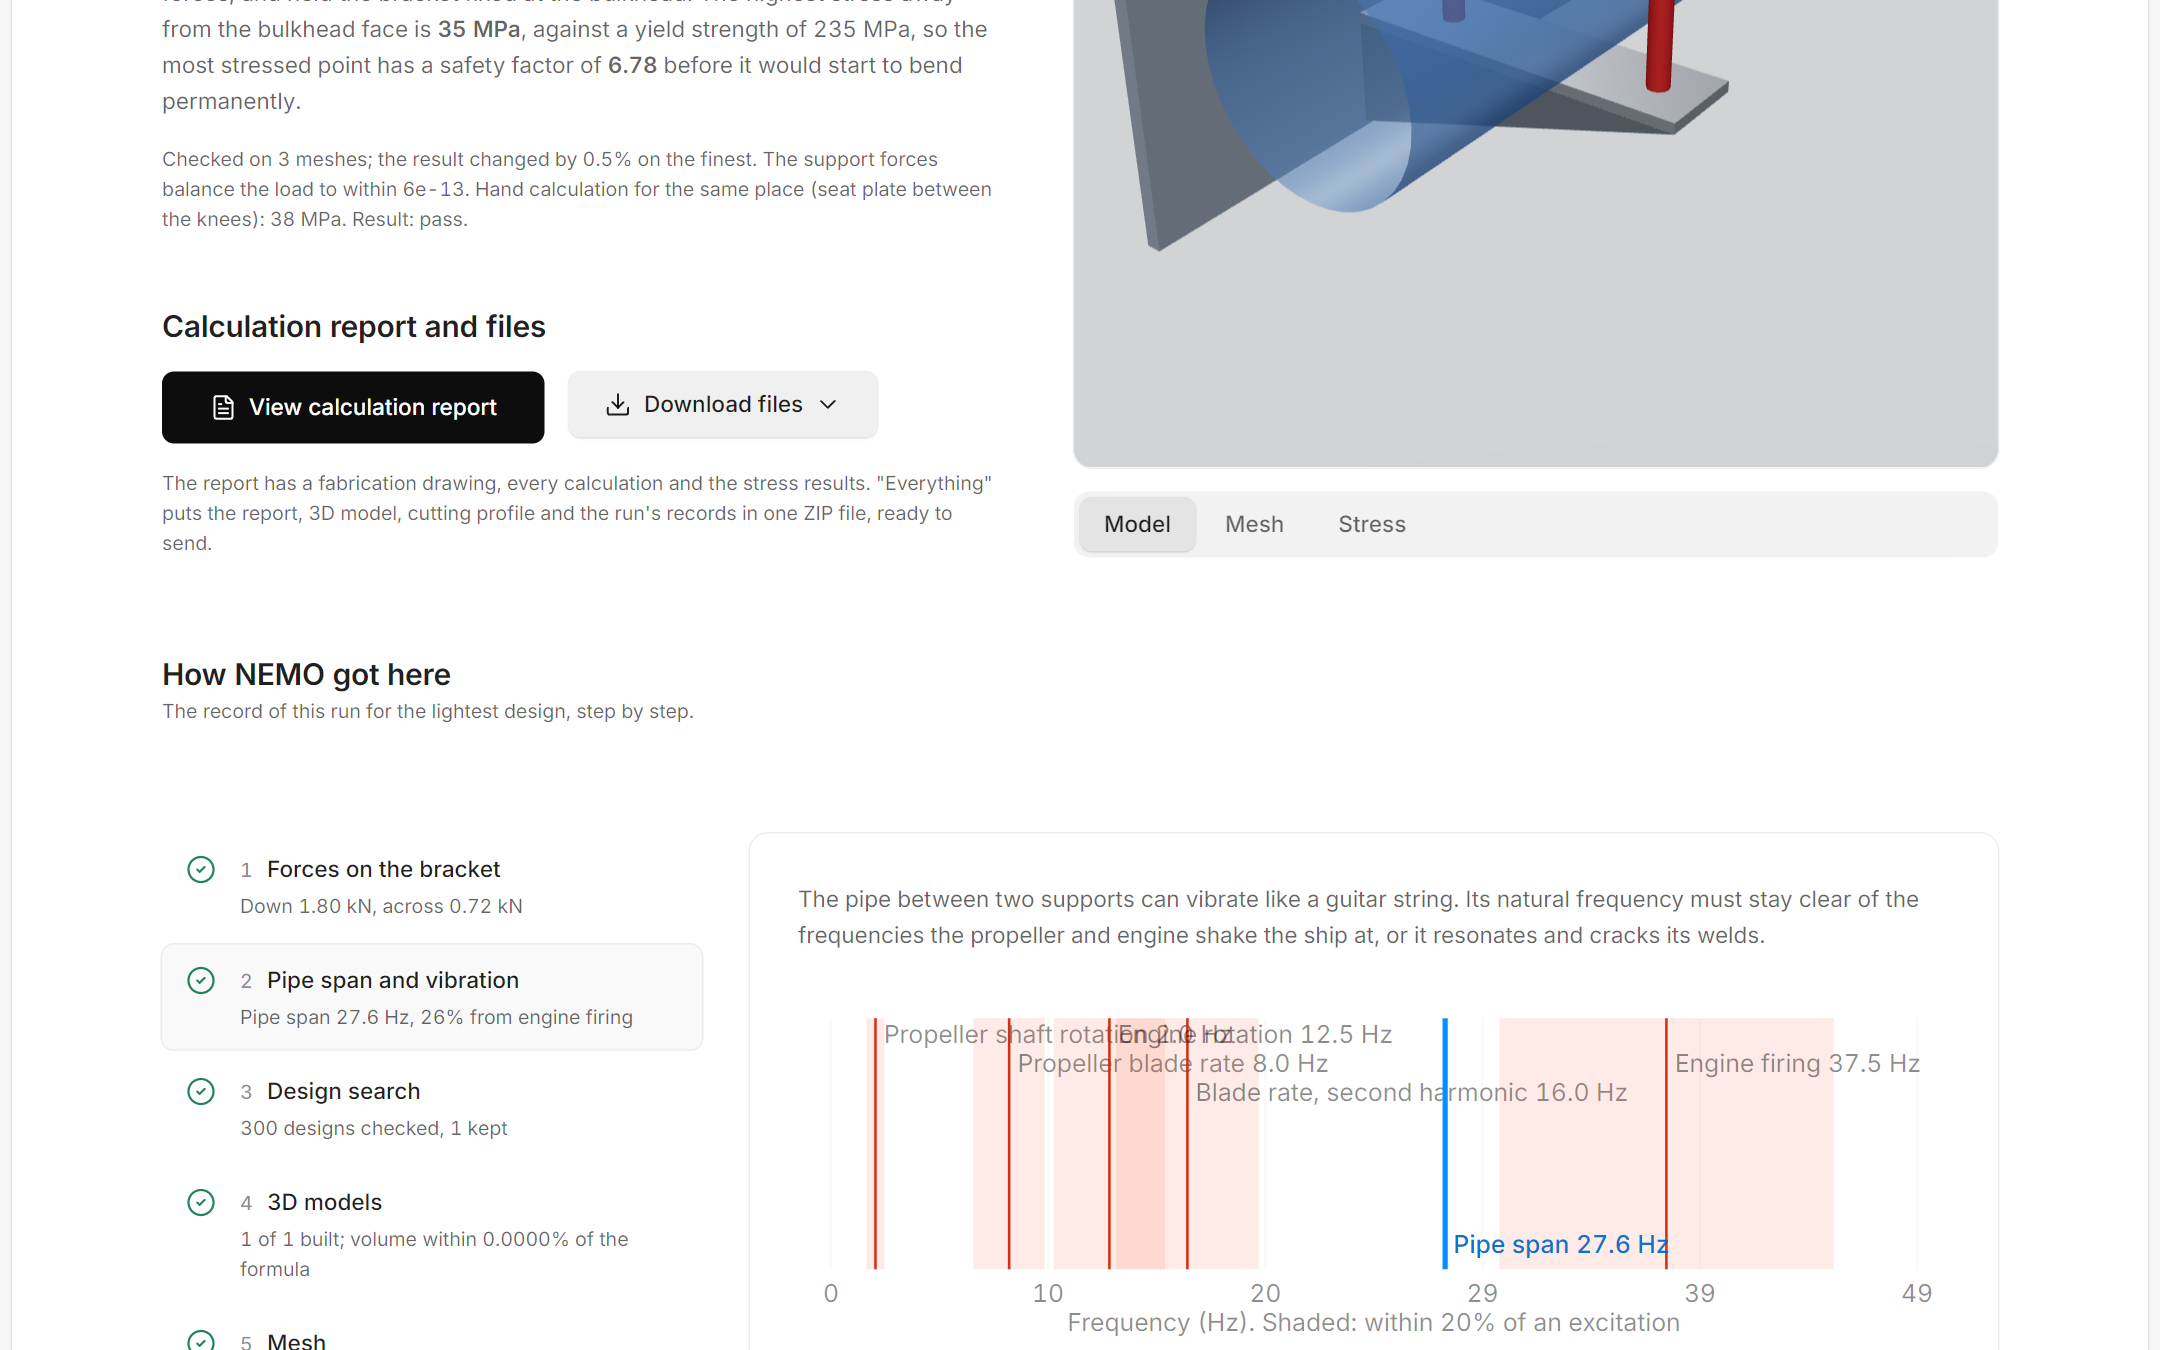
\includegraphics[width=\textwidth]{images/app-bracket-record.png}
\caption{Bracket engineering record}
\end{subfigure}
\caption{Fin and bracket results screens}
\label{fig:app-record}
\end{figure}

\section{Run times}
\label{sec:run-times}

Table~\ref{tab:run-times} gives the run times on the development computer,
running Windows. A run includes the search for all three targets, the CAD, the
three finite element solves for each design and the PDF packages.

\begin{table}[H]
\centering
\caption{Run times of the case studies}
\label{tab:run-times}
\small
\begin{tabular}{lrrrr}
\toprule
\textbf{Run} & \textbf{Designs tried} & \textbf{Kept} & \textbf{Largest model, unknowns} & \textbf{Time (s)}\\
\midrule
Padeye & 19,389 & 3 & 209,763 & 138.2\\
Bracket & 300 & 1 & 97,380 & 29.8\\
Fin & 3,780 & 3 & 75,831 & 79.9\\
Verification suite & & & 96,000 & 27.9\\
\bottomrule
\end{tabular}
\end{table}

Most of the padeye time is in the finite element solves. The three meshes of
the lightest design took 44~s together, and the finest mesh, with 209,763
unknowns, took 26.9~s. The search itself, 19,389 check evaluations, takes
less time than the analysis of one design. The live run screen shows progress
throughout, so the user can see which step is running and what it has found.

\section{Comparison with the first phase}
\label{sec:comparison}

Table~\ref{tab:comparison} compares the two phases against the requirements
of Table~\ref{tab:requirements}.

\begin{table}[H]
\centering
\caption{\NEMO{}~1 and \NEMO{}~2 compared}
\label{tab:comparison}
\small
\begin{tabularx}{\textwidth}{>{\raggedright\arraybackslash}p{0.2\textwidth}>{\raggedright\arraybackslash}X>{\raggedright\arraybackslash}X}
\toprule
\textbf{Aspect} & \textbf{\NEMO{}~1} & \textbf{\NEMO{}~2}\\
\midrule
Parts & Aluminium bracket, S275 padeye, aluminium fin & Steel padeye, pipe support bracket with pipe span, fin internal structure and stock\\
Design basis & Screening equations, some with unsourced factors & ASME BTH-1, AISC 360-16 and IACS UR S10 through replaceable rule sets; practice checks labelled\\
Fin load & Assumed & Whicker-Fehlner and UR S10, larger used; panel method for pressure and cavitation\\
Optimiser & Latin hypercube and Nelder-Mead on continuous variables & Stock plate enumeration, bounded Nelder-Mead, rounding, three targets\\
Stress analysis & Fusion Simulation, set up by hand; two bracket studies rejected & Built-in, three meshes per design, force balance and convergence checked automatically\\
Verification & None recorded & Six benchmarks with 24 compared quantities, and 153 automated tests\\
Traceability & Result files & Working for every check, engineering log, every design tried, checksums\\
Use & Python, virtual environment and Fusion needed & Installer and browser application; Fusion optional\\
Fusion link & File bridge that rebuilt stale requests & HTTP polling with expiring jobs; parametric model and re-check of edits\\
\bottomrule
\end{tabularx}
\end{table}

\section{Answers to the research questions}
\label{sec:research-answers}

\textbf{RQ1. Can one tool cover three structurally different marine details
while keeping every check traceable to a named rule or a stated practice?}
Yes, for the three parts built. The common check record, the rule-set
interface and the shared sizing and analysis pipeline served a pin-loaded
plate, a cantilever bracket with a vibration problem and a hydrodynamic foil
on a stock. Every check in Tables~\ref{tab:padeye-checks},
\ref{tab:bracket-checks-result} and~\ref{tab:fin-checks-result} names its
source, and the practice checks are labelled. The parts differ enough that
each needed its own load model and its own finite element set-up, so a new
part is still a substantial piece of work.

\textbf{RQ2. How closely do the built-in stress solver, geometry kernel and
foil solver agree with closed-form and published reference results?} The
geometry agrees exactly. The stress solver agrees within 0.8\% for
deflection, 2.6\% for beam stress, 0.9\% for a stress concentration and
0.13\% for the stock. The foil solver agrees within 0.05\% for the circle and
1.1\% to 1.7\% for the lift slope estimate. Force balance closed to
$10^{-11}$ or better on every model. These results show that the solvers are
implemented correctly. They do not validate the idealisations of the models,
such as the fixed supports or the cosine pin pressure.

\textbf{RQ3. What governs each part in practice, and what does that imply for
how such details are designed?} For the padeye, the base weld and the shackle
rating govern at moderate loads, and splitting above the hole at large loads.
Catalogue steps in the shackle drive the mass more than the plate dimensions.
For the bracket, minimum sizes govern the steel and pipe vibration governs the
spacing. Its strength checks reach only 25\%, while the span frequency limits
spacing to 2.3~m and the pass or fail result is not monotonic in spacing.
For the fin, the stock governs through the rule limit on combined stress, the
plating sits at rule minimums, the foil load exceeds the rule load by 21\%, and
cavitation limits the largest angle above about 18~knots. The common
implication is that a design method for these details must include the minimum
sizes, the catalogue and stock steps, the span and the hydrodynamics. A method
that only minimises mass under strength checks would miss what decides the
design in each case.

\textbf{RQ4. Can a non-programmer run the full workflow, from job description
to calculation package, unaided?} The tool removes the technical barriers. It
installs from one file, the forms ask for the job in plain words, and the run,
results and package need no code. Whether a non-programmer can complete the
workflow unaided has not been tested with users. A formal usability study is
needed to answer this question, and it is listed in
Section~\ref{sec:future-work}.

\section{Limitations}
\label{sec:limitations}

The results above have the following limits, which a user of the tool should
know.

\begin{itemize}
    \item \textbf{No physical tests.} All verification is against hand
    calculations, theory and published coefficients. No padeye, bracket or fin
    designed by the tool has been built or load tested.
    \item \textbf{BTH-1 reading not checked against a worked example.} The code
    matches the engineering manual, but the manual has not been compared with
    a published BTH-1 padeye example.
    \item \textbf{Ship-motion accelerations are inputs.} The bracket loads are
    only as good as the accelerations the user enters. The tool does not
    compute them from a classification society method.
    \item \textbf{Simplified span model.} The pipe span is treated as a simply
    supported beam on rigid supports. Flexible supports, bends, valves and
    fluid flow change the frequency and are not modelled.
    \item \textbf{Quasi-static fin loads.} The fin is checked under the steady
    load at its largest angle. Dynamic loads from fin motion, waves, slamming
    and the control system are not included. The panel method is inviscid and
    gives cavitation onset only.
    \item \textbf{Rudder rules applied to a fin.} UR S10 is written for
    rudders. It is the nearest published basis, but its use does not amount to
    class approval of a fin.
    \item \textbf{Finite element scope.} The finite element models are linear
    elastic, do not include the welds, and model the fin stock alone. They
    confirm the hand checks in the regions they cover.
    \item \textbf{Fusion connector untested in Fusion.} The add-in has not yet
    been run in a live Fusion session, and no Fusion stress cross-check has
    been recorded.
    \item \textbf{No usability study.} Ease of use has been designed for but
    not measured.
\end{itemize}

\chapter{Project workplan}
\label{chap:workplan}

This chapter presents the project schedule from September 2026 to March 2027,
tracing the work from marine code review and exploratory CAD trials through
engine implementation, verification, case studies and final reporting.

\section{Schedule}
\label{sec:schedule}

Figure~\ref{fig:gantt} shows the schedule in half-month intervals. September
and October were devoted to reviewing the marine design standards, testing
preliminary screening models and conducting early Autodesk Fusion integration
trials. Those early tests confirmed that the public Fusion API could not
automate simulation set-up and solving, and two manual bracket studies had to
be rejected because of input errors. That finding fixed the architecture of
\NEMO{} around a self-contained, open-source geometry and finite element
pipeline.

From November onward, development followed the three project objectives in
order. November and December established the shared calculation core, the ASME
BTH-1 lifting padeye module, the automated quadratic finite element pipeline
and the local browser application. January added the AISC 360-16 pipe support
bracket with machinery-space vibration screening, the IACS UR S10 stabilizer
fin with foil-load and cavitation models, and the reproducible verification
benchmark suite. February covered the three vessel case studies, parameter
sweeps, finite element verification and validation checks, user documentation
and the Windows installer. March is reserved for final corrections, project
demonstration and submission. Report writing ran alongside the engineering
work so that equations, decisions and numerical evidence were captured as each
stage completed.

\begin{figure}[H]
\centering
\begin{ganttchart}[
    hgrid,
    vgrid,
    x unit=0.64cm,
    y unit title=0.62cm,
    y unit chart=0.52cm,
    title label font=\bfseries\scriptsize,
    bar label font=\scriptsize,
    group label font=\bfseries\scriptsize,
    milestone label font=\scriptsize,
    bar/.append style={fill=nemoblue!35,draw=nemoblue},
    group/.append style={fill=nemoteal!35,draw=nemoteal},
    milestone/.append style={fill=nemoorange,draw=nemoorange}
]{1}{14}
\gantttitle{2026}{8}\gantttitle{2027}{6}\\
\gantttitle{Sep}{2}
\gantttitle{Oct}{2}
\gantttitle{Nov}{2}
\gantttitle{Dec}{2}
\gantttitle{Jan}{2}
\gantttitle{Feb}{2}
\gantttitle{Mar}{2}\\

\ganttgroup{Foundation and early testing}{1}{4}\\
\ganttbar{Marine codes and literature}{1}{2}\\
\ganttbar{Exploratory CAD and FEA trials}{2}{4}\\
\ganttmilestone{Architecture frozen}{4}\\

\ganttgroup{Engine, verification and cases}{5}{12}\\
\ganttbar{Core rules and padeye sizing (O1)}{5}{6}\\
\ganttbar{CAD--FEA pipeline and app (O1, O2)}{7}{8}\\
\ganttbar{Bracket, fin and verification (O1, O2)}{9}{10}\\
\ganttbar{Case studies and V\&V checks (O2, O3)}{10}{12}\\
\ganttbar{Documentation and installer}{11}{12}\\

\ganttgroup{Reporting}{1}{14}\\
\ganttbar{Report writing}{1}{14}\\
\ganttbar{Corrections, demonstration}{13}{14}\\
\ganttmilestone{Submission}{14}
\end{ganttchart}
\caption{Project workplan, September 2026 to March 2027, in half-months}
\label{fig:gantt}
\end{figure}

\section{Workplan review}
\label{sec:workplan-review}

The main schedule adjustment occurred at the end of October, when the early
Fusion trials showed that automated stress confirmation required a local
open-source solver. Adopting build123d, Gmsh and scikit-fem required upfront
integration work in November and December, but it removed the manual transfer
step that had caused earlier load-input errors. Completing the lifting padeye
end to end before starting the pipe bracket and stabilizer fin also paid off:
by January, the common check record, stock-aware sizing search, three-mesh
finite element routine, engineering log and PDF report builder were already
tested and reused directly by the remaining two parts. All tasks tied to the
three project objectives were completed within schedule; optional extensions
outside the verified software scope, including physical proof testing and a
formal user study, are documented as future work.

\chapter{Project budget}
\label{chap:budget}

This chapter gives the direct cash budget and the resources the project used
without paying for them. The project was planned around computers the
authors already had, open-source engineering software, Autodesk educational
access and digital submission, so its direct cash budget is zero.

\section{Direct cash budget}
\label{sec:budget}

No equipment, software licence, cloud service, data, printing, travel,
fabrication or testing was paid for from project funds.
Table~\ref{tab:cash-budget} sets out the reasons.

\begin{table}[H]
\centering
\caption{Direct cash budget}
\label{tab:cash-budget}
\small
\begin{tabularx}{\textwidth}{
    >{\raggedright\arraybackslash}p{0.23\textwidth}
    >{\raggedright\arraybackslash}X
    >{\centering\arraybackslash}p{0.15\textwidth}}
\toprule
\textbf{Category} & \textbf{Why no cash is needed} & \textbf{Budget (KES)}\\
\midrule
Computers & Existing personal and university computers. The finite element models were kept small enough to solve on them, the largest at 209,763 unknowns in under a minute. & 0\\[0.35em]
CAD and analysis software & build123d, OpenCASCADE, Gmsh, scikit-fem and PyAMG are open source and provide the automated geometry and stress-analysis pipeline locally. & 0\\[0.35em]
Autodesk Fusion & Educational access, used for early exploratory trials and for the optional CAD connector. & 0\\[0.35em]
Other software & Python, NumPy, SciPy, FastAPI, ReportLab, React, three.js, Git and LaTeX are free to use. & 0\\[0.35em]
Cloud services & Everything runs on the user's computer. No paid hosting or remote computation is used. & 0\\[0.35em]
Internet and electricity & Existing personal and university services. & 0\\[0.35em]
Printing and travel & The report is submitted digitally. & 0\\[0.35em]
Fabrication and testing & Physical fabrication and load testing are outside the scope of this project. & 0\\[0.35em]
Contingency & Schedule margin and scope control instead of a cash reserve. & 0\\
\midrule
\textbf{Total} & & \textbf{0}\\
\bottomrule
\end{tabularx}
\end{table}

\section{In-kind resources}
\label{sec:in-kind-resources}

A zero cash budget does not mean the project used no resources.
Table~\ref{tab:in-kind} lists them. They are not given money values, because
there is no sound basis for pricing them.

\begin{table}[H]
\centering
\caption{In-kind resources}
\label{tab:in-kind}
\small
\begin{tabularx}{\textwidth}{
    >{\raggedright\arraybackslash}p{0.25\textwidth}
    >{\raggedright\arraybackslash}X
    >{\raggedright\arraybackslash}X}
\toprule
\textbf{Resource} & \textbf{How it was provided} & \textbf{What it was used for}\\
\midrule
Computers & Personal and university & Development, automated tests, case studies, report\\
Open-source software & Public licences & Geometry, meshing, finite element analysis, server, application, report\\
Autodesk Fusion & Educational access & Early CAD and simulation trials; optional parametric padeye connector\\
Design codes and catalogues & University library and public sources & Rule sets, material grades, shackle and pipe reference data\\
Internet and electricity & Personal and university & Research, package downloads, running the tool\\
Student time and supervision & Academic project & Marine engineering analysis, programming, verification and writing\\
\bottomrule
\end{tabularx}
\end{table}

\section{Costs beyond this project}
\label{sec:budget-beyond}

Taking a design from \NEMO{} into shipboard service requires expenditure outside
this academic project. A proof load test of a lifting padeye, vibration
measurements on an engine-room pipe run, model basin or sea trials of a
stabilizer fin, certified marine steel plate, fabrication and non-destructive
weld inspection each carry their own yard and survey costs. A commercial
organisation adopting the tool would also need licensed copies of the
referenced design codes: ASME BTH-1, AISC 360 and AWS D1.1 are sold by their
publishers, whereas IACS Unified Requirements are freely published.

\chapter{Conclusions and recommendations}
\label{chap:conclusion}

This chapter states what the project achieved against each objective, what
the results mean for the design of these details, and what should be done
next.

\section{Conclusions}
\label{sec:conclusions}

The project set out to build and verify a desktop tool that sizes three
marine structural details from a plain description of the job, checks them
against published rules, confirms them with a built-in finite element
analysis and issues a calculation package that a non-programmer can produce
and review. \NEMO{}~2 does this for lifting padeyes, pipe support brackets and
stabilizer fins. The objectives were met as follows.

\begin{enumerate}
    \item \textbf{Rule-based check models.} The padeye is checked to ASME
    BTH-1, the bracket to AISC 360-16 in allowable strength design with a
    check of the pipe span against five machinery excitations, and the fin to
    IACS UR S10 with a Whicker-Fehlner foil load and a Hess-Smith panel method.
    Every check returns its working and names its source, and the 15 padeye,
    14 bracket and 11 fin checks separate code rules from practice. Objective
    1 was met.
    \item \textbf{Stock-aware sizing.} The search enumerates the plate stock,
    shackles, U-bolts and weld sizes, sizes the continuous dimensions with a
    bounded Nelder-Mead search, rounds to buildable sizes and returns designs
    at 100\%, 85\% and 70\% maximum use. Lower-bound pruning skipped 60 of 63
    combinations in the bracket case. Objective 2 was met.
    \item \textbf{Open-source geometry and analysis.} Every design is built as
    an exact solid, meshed three times and solved with quadratic tetrahedra.
    Force balance closed to $10^{-11}$ or better and the assessed peak changed
    by 0.54\% or less between the two finest meshes in all three case studies.
    The manual stress step that blocked the first phase is gone. Objective 3
    was met.
    \item \textbf{Verification.} The engine matches a padeye hand calculation
    within 0.002\%, CAD volumes exactly, beam theory within 2.6\%, a published
    stress concentration factor within 0.9\% and foil theory within 1.7\%. All
    174 automated tests pass. Objective 4 was met for code verification. A
    comparison with a published BTH-1 worked example is still to be done.
    \item \textbf{Interface and outputs.} The tool installs from one file and
    runs in the browser. It shows the engineering steps live, gives the
    working of every check, and writes a PDF package, STEP, STL and DXF files.
    The Fusion connector builds a parametric padeye and re-checks edited
    dimensions. Objective 5 was met in build. In its first Fusion session the
    connector built a padeye with the same volume as \NEMO{}'s, but no agreeing
    stress cross-check has been made yet, and ease of use has not been measured with
    users.
    \item \textbf{Case studies.} One case per part was run, with sweeps of
    load, sling angle, pipe size, support spacing and ship speed, and the
    limits of the results were stated in Section~\ref{sec:limitations}.
    Objective 6 was met.
\end{enumerate}

The case studies also gave findings about the parts themselves.

\begin{itemize}
    \item A 5~t two-point padeye weighs 0.305~kg and is governed by its base
    weld at 98\%. Asking for 15\% spare capacity raises the mass by 42\%,
    because the shackle has to move up a size. Catalogue steps, more than plate
    dimensions, set the mass of small lifting details.
    \item An NPS~4 seawater line bracket uses 25\% of its strength and is
    sized by minimum plate, weld and U-bolt sizes. Its pipe span limits support
    spacing to 2.3~m because of engine firing at 37.5~Hz. Shortening the 3~m
    span to 2.5~m would move it into resonance, so pass or fail does not
    improve steadily as spacing falls.
    \item An oblique sling at 45$^\circ$ to the plate of the 5~t padeye cuts the
    shackle's rating to 75\% and raises the mass by 41\%. For large pipes the
    bracket's own flexibility lowers the span frequency by up to a quarter.
    Close stock bearings can make the fin stock larger than the stress rules
    alone would.
    \item For a 1.4~m by 1.2~m fin at 18~knots, the foil model gives a force
    21\% above the UR S10 rudder formula. The stock governs at 94.5\%, the
    plating sits at rule minimums, and leading-edge cavitation begins between
    18 and 20~knots at the largest angle.
\end{itemize}

The common lesson is that a design method for these details cannot stop at
strength. Minimum sizes, catalogue steps, pipe vibration and foil
hydrodynamics decided the design in every case study.

\section{Recommendations}
\label{sec:recommendations}

For engineers using \NEMO{}~2:

\begin{itemize}
    \item Use the calculation package as a checked starting point, and have a
    competent engineer review it before fabrication. The package is written so
    that the review can be done without the software.
    \item Enter ship-motion accelerations from the classification society
    rules for the vessel, not the defaults, when designing brackets.
    \item Treat the recommended support spacing as the limit for pipe runs
    near machinery, even where the actual spacing passes the separation check.
    \item For fins, use the larger of the two load methods, as the tool does,
    and treat a cavitation warning as a limit on the largest fin angle at that
    speed.
    \item Run the Verification page after installing the tool on a new
    computer, and keep its result with the project file.
\end{itemize}

For the department:

\begin{itemize}
    \item The tool could be used in teaching structural design of ship
    details, because every check shows its working and the effect of an input
    can be seen in a few minutes.
    \item Future projects could add parts to the same engine, such as
    foundations for small machinery or deck fittings, using the existing check
    record, rule sets, sizing method and analysis pipeline.
\end{itemize}

\section{Future work}
\label{sec:future-work}

\begin{enumerate}
    \item Compare the padeye checks with a published ASME BTH-1 worked
    example.
    \item Repeat the Fusion Static Stress cross-check of a padeye with
    connector version 1.1.0, which sets the material in Fusion, and record an
    agreeing result. Extend the connector to brackets and fins.
    \item Carry out a usability study in which marine engineering students who
    have not used the tool complete a design from job description to
    calculation package, and record their time, errors and comments.
    \item Proof load test a padeye designed by the tool, with strain gauges
    near the hole, to validate the finite element model.
    \item Compute bracket accelerations from a classification society method,
    such as the DNV rules for ship motions, from the vessel's main dimensions.
    \item Extend the pipe span model to continuous runs with bends, valves and
    flexible supports.
    \item Add dynamic and fatigue checks for the fin, and a model of the whole
    fin, not only the stock, in the finite element analysis.
    \item Add rule sets from classification societies, such as DNV, Lloyd's
    Register and Bureau Veritas, through the existing rule-set interface.
\end{enumerate}


\clearpage

% ==============================================================================
% REFERENCES AND APPENDICES
% ==============================================================================

\bibliographystyle{IEEEtran}
\bibliography{references}

\appendix
\chapter{Engine source structure}
\label{app:source}

Table~\ref{tab:app-source} lists the modules of the engine with their size
in lines. The shared modules sit at the top of the package and each part has
its own sub-package with the modules described in
Table~\ref{tab:part-modules}.

\begin{longtable}{>{\raggedright\arraybackslash}p{0.36\textwidth}r>{\raggedright\arraybackslash}p{0.46\textwidth}}
\caption{Engine modules}\label{tab:app-source}\\
\toprule
\textbf{Module} & \textbf{Lines} & \textbf{Purpose}\\
\midrule
\endfirsthead
\toprule
\textbf{Module} & \textbf{Lines} & \textbf{Purpose}\\
\midrule
\endhead
\code{checks.py} & 117 & Common check record and part report\\
\code{loads.py} & 126 & Padeye loads, including the oblique sling\\
\code{working.py} & 59 & Working steps for checks\\
\code{hydro.py} & 127 & Hess-Smith panel method and cavitation number\\
\code{fea/mesh.py} & 129 & Gmsh meshing of STEP solids\\
\code{fea/solver.py} & 356 & P2 elasticity, traction loads, tensor nodal stress, 6-DOF balance, direct and multigrid solvers\\
\code{fea\_study.py} & 128 & Three-mesh study, convergence and force balance\\
\code{optimize/nelder\_mead.py} & 89 & Bounded Nelder-Mead search\\
\code{rules/asme\_bth1.py} & 193 & ASME BTH-1 rule set\\
\code{rules/aisc360.py} & 66 & AISC 360-16 ASD rule set\\
\code{rules/iacs\_s10.py} & 87 & IACS UR S10 rule set, astern factors and bearing limits\\
\code{data/} & 174 & Loader for materials, shackles, pipes and plate stock; shackle side-load table\\
\code{parts/registry.py} & 137 & List of parts for the server and application\\
\code{parts/padeye/} & 2,166 & Padeye job, geometry, checks, working, sizing, CAD, DXF, FEA, Fusion model\\
\code{parts/bracket/} & 1,467 & Bracket job, pipe span, bracket flexibility, geometry, checks, sizing, CAD, FEA\\
\code{parts/stabilizer/} & 1,129 & Fin job, loads ahead and astern, bearings, geometry, checks, sizing, CAD, FEA\\
\code{report\_pdf.py} & 998 & PDF calculation package for the padeye, and shared page layout\\
\code{report\_parts.py} & 582 & PDF sections for the bracket and the fin, with their Fusion cross-check\\
\code{projects.py} & 188 & Projects, runs and their folders\\
\code{runlog.py} & 76 & Engineering log\\
\code{verification.py} & 269 & Benchmark suite\\
\code{server.py} & 539 & Local web server\\
\code{fusion\_link.py} & 181 & Fusion job queue\\
\code{fusion\_sheet.py} & 163 & Fusion cross-check sheet\\
\bottomrule
\end{longtable}

\chapter{Automated tests}
\label{app:tests}

Table~\ref{tab:app-tests} lists the test files. Some tests run once for each
of several inputs, which is why the CAD file holds 54 tests. All 181 tests
pass.

\begin{table}[H]
\centering
\caption{Automated tests}
\label{tab:app-tests}
\small
\begin{tabularx}{\textwidth}{lrX}
\toprule
\textbf{File} & \textbf{Tests} & \textbf{What is tested}\\
\midrule
\code{test\_padeye\_hand\_calc.py} & 7 & Every BTH-1 quantity against the hand calculation\\
\code{test\_padeye\_behaviour.py} & 19 & Each check responds correctly when one input changes\\
\code{test\_padeye\_cad.py} & 54 & Solid volume against the formula for random designs; STEP export and re-import\\
\code{test\_padeye\_fea.py} & 6 & Padeye finite element model, force balance, convergence, fast assembly\\
\code{test\_padeye\_sizing.py} & 9 & Sizing results, targets, rounding, stock and shackle choices\\
\code{test\_fea\_benchmarks.py} & 2 & Cantilever and plate with a hole\\
\code{test\_fea\_vv\_regressions.py} & 7 & 6-DOF equilibrium, zero-moment axial side load, cheek-step exclusion, tensor nodal stress, Frocht--Hill pin-loaded lug $K_{tn}$ benchmark, Fusion unit guards and cross-check sheet\\
\code{test\_bracket.py} & 9 & Bracket loads, pipe span, checks, sizing and FEA\\
\code{test\_stabilizer.py} & 11 & Fin loads, panel method, checks, sizing and stock FEA\\
\code{test\_transparency.py} & 9 & Working results equal check values; engineering log and design records\\
\code{test\_projects\_pipeline.py} & 7 & Projects, runs and output files\\
\code{test\_server.py} & 8 & Server routes for the padeye\\
\code{test\_server\_parts.py} & 6 & Server routes for the bracket and the fin\\
\code{test\_fusion\_link.py} & 7 & Fusion job queue, pickup and expiry, material record, refused reactions\\
\code{test\_advanced\_settings.py} & 20 & Oblique sling and shackle side loading, bracket flexibility, fin astern condition and bearings, by hand\\
\midrule
\textbf{Total} & \textbf{181} & \\
\bottomrule
\end{tabularx}
\end{table}

\chapter{Case-study job descriptions}
\label{app:jobs}

The engine stores each job as a JSON file. Listing~\ref{lst:padeye-job}
shows the job of the padeye case study as the engine saved it. The bracket and
fin jobs have the same form with their own fields, listed in
Table~\ref{tab:cases}.

\begin{lstlisting}[language={}, caption={Job description of the padeye case study}, label={lst:padeye-job}]
{
  "part": "padeye",
  "lift": {
    "lifted_mass_kg": 5000.0,
    "lift_points": 2,
    "sling_angle_deg": 60.0,
    "dynamic_factor": 1.0,
    "points_carrying": null,
    "side_load_fraction": 0.05
  },
  "material_id": "S355",
  "plate_thicknesses_mm": [6, 8, 10, 12, 15, 20, 25, 30, 40, 50],
  "allow_cheek_plates": true,
  "rule_set_id": "asme-bth-1",
  "design_category": "B",
  "service_class": 0,
  "fill_shackle_jaw": true,
  "electrode_strength_mpa": 482.0
}
\end{lstlisting}

\chapter{Selected source code}
\label{app:code}

Listing~\ref{lst:nelder-mead} shows the main loop of the bounded Nelder-Mead
search described in Section~\ref{sec:sizing}. Every trial point is clipped to
the unit box, and values are cached so that a repeated point is not evaluated
twice.

\begin{lstlisting}[language=Python, caption={Main loop of the bounded Nelder-Mead search, from \code{optimize/nelder\_mead.py}}, label={lst:nelder-mead}]
for iterations in range(1, max_iter + 1):
    order = sorted(range(n + 1), key=lambda i: values[i])
    simplex = [simplex[i] for i in order]
    values = [values[i] for i in order]
    if abs(values[-1] - values[0]) <= tolerance * (abs(values[0]) + 1e-12):
        spread = max(max(abs(a - b) for a, b in zip(v, simplex[0])) for v in simplex[1:])
        if spread < 1e-4:
            break

    centroid = [sum(v[d] for v in simplex[:-1]) / n for d in range(n)]
    worst = simplex[-1]
    reflected = _clip([c + (c - w) for c, w in zip(centroid, worst)])
    fr = f(reflected)
    if values[0] <= fr < values[-2]:
        simplex[-1], values[-1] = reflected, fr
        continue
    if fr < values[0]:
        expanded = _clip([c + 2.0 * (r - c) for c, r in zip(centroid, reflected)])
        fe = f(expanded)
        simplex[-1], values[-1] = (expanded, fe) if fe < fr else (reflected, fr)
        continue
    contracted = _clip([c + 0.5 * (w - c) for c, w in zip(centroid, worst)])
    fc = f(contracted)
    if fc < values[-1]:
        simplex[-1], values[-1] = contracted, fc
        continue
    best = simplex[0]
    for i in range(1, n + 1):
        simplex[i] = _clip([b + 0.5 * (v - b) for b, v in zip(best, simplex[i])])
        values[i] = f(simplex[i])
\end{lstlisting}

Listing~\ref{lst:check-record} shows the common check record of
Section~\ref{sec:check-model}.

\begin{lstlisting}[language=Python, caption={Common check record, from \code{checks.py}}, label={lst:check-record}]
@dataclass(frozen=True)
class CheckResult:
    id: str
    title: str
    demand: float
    capacity: float
    unit: str
    source: str
    explanation: str
    basis: Basis = "rule"            # "rule" or "practice"
    severity: Severity = "required"  # "required" or "advice"
    category: Category = "strength"  # "strength", "fit", "stiffness", "span"
    details: dict[str, float] = field(default_factory=dict)
    working: tuple = ()

    @property
    def utilization(self) -> float:
        if self.capacity <= 0:
            return float("inf")
        return self.demand / self.capacity

    @property
    def passed(self) -> bool:
        return bool(self.utilization <= 1.0 + 1e-12)
\end{lstlisting}

\chapter{Using \NEMO{}}
\label{app:user-steps}

The steps below summarise the user guide that comes with the tool.

\begin{enumerate}
    \item Double-click \code{Install NEMO.bat}. This is needed once and
    requires an internet connection.
    \item Double-click the NEMO shortcut on the desktop, or
    \code{Start NEMO.bat}. The application opens in the browser.
    \item Press \emph{New design} and choose the part (Figure~\ref{fig:app-new}).
    \item Fill in the job description. The 3D preview updates as values
    change. Tick the plate thicknesses the workshop holds.
    \item Check the assumptions and change any that do not fit the job.
    \item Press \emph{Find designs} and follow the run on the live screen.
    \item Compare the three designs, open the checks to see their working,
    and download the PDF package and the STEP and DXF files.
    \item Optionally, send a padeye to Fusion to edit it there and check the
    edited design in \NEMO{}.
\end{enumerate}

\begin{figure}[H]
\centering
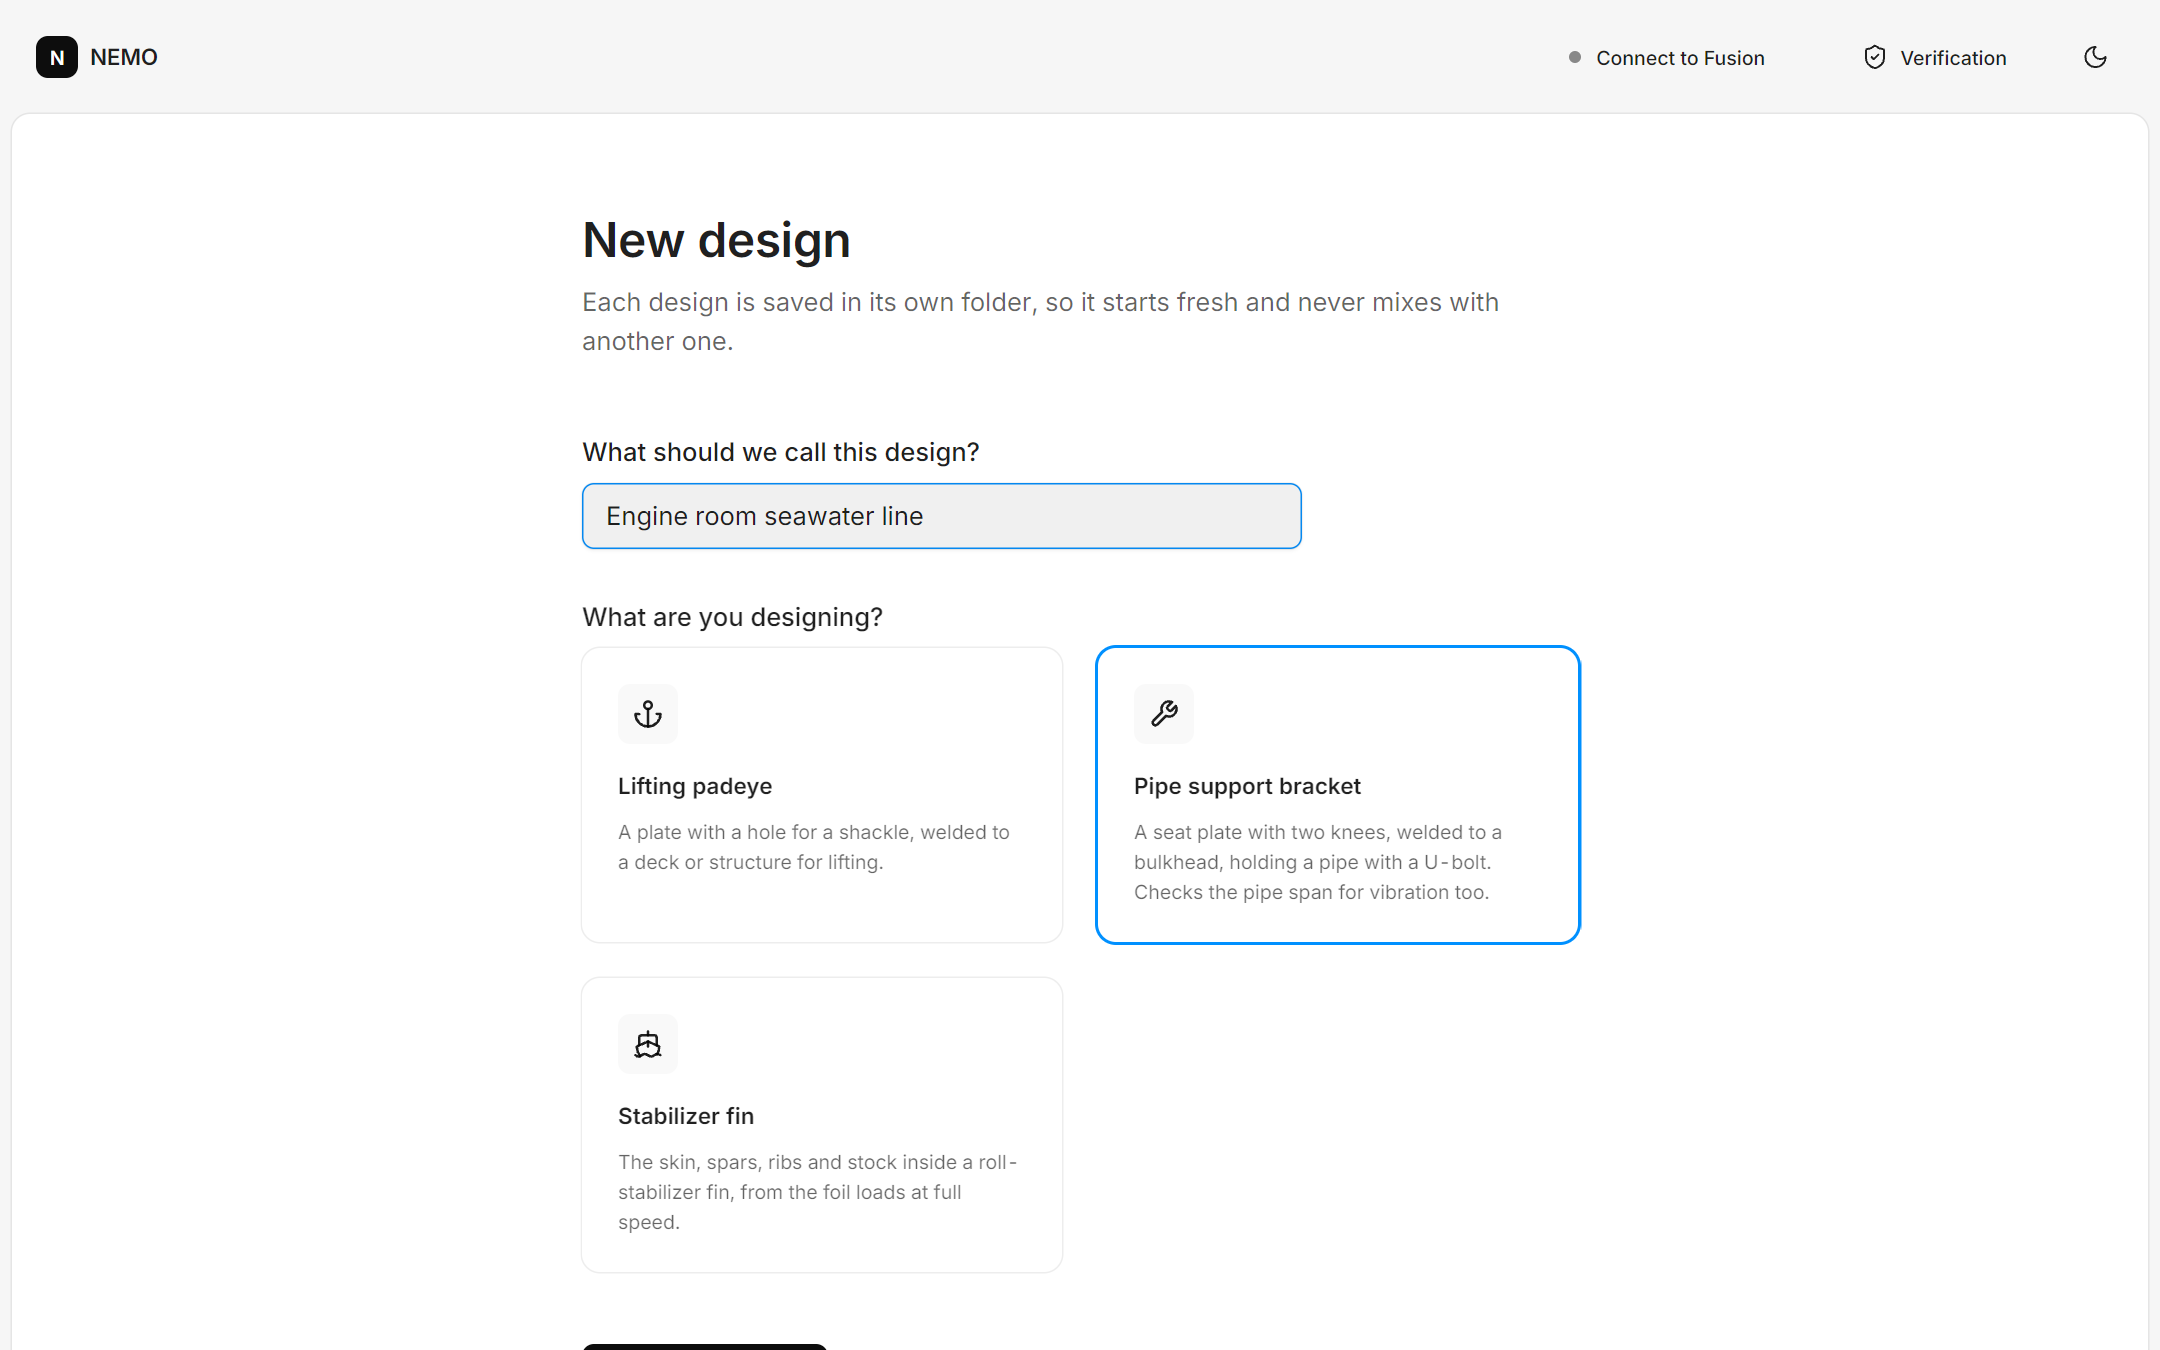
\includegraphics[width=\textwidth]{images/app-new-design.png}
\caption{Choosing the part for a new design}
\label{fig:app-new}
\end{figure}


\end{document}
